\section{Kodierung}

Wie bereits geschrieben wurde die Erstkodierung von David Sichau durchgeführt. Es wurden eine Zweitkodierung von  15 \% zufällig ausgewählten (per Random Generator) Auswertungsbögen von Pitt Hild  durchgeführt. Es wurden dabei die gleichen Kodierschemata verwendet, welche sich im Anhang der Arbeit befinden (siehe Sektion \ref{sec:Kodierung} im Anhang). 

\subsection{Items}
Es gab insgesamt elf Items welche nach dem Kodierschemata kodiert wurden.

Die Items wurden auf Interrater-Reliabilität untersucht. Dafür wurden die prozedurale Übereinstimmung $p_0$ und zusätzlich noch das ungewichtete Cohen's Kappa $\kappa$ als Zufalls-korrigierter Koeffizient berechnet. Bei einem Teil der Datensätze war dies mathematisch nicht möglich (Division durch 0), daher können nicht für alle Items ein Cohen's Kappa angegeben werden. In Tabelle \ref{tab:CohenKappa} sind alle Ergebnisse zusammengefasst.


\github{http://git.io/mk9z-Q}

\begin{table}[htbp]
  \centering
\begin{tabular}{@{}lllllllll@{}}
\toprule   &  \multicolumn{2}{c}{201} &&  \multicolumn{2}{c}{301}  && \multicolumn{2}{c}{301}\\
 \cmidrule{2-3}  \cmidrule{5-6} \cmidrule{8-9}
Item  & $p_0$ & $\kappa$ &&  $p_0$ & $\kappa$ &&  $p_0$ & $\kappa$\\
\midrule
 1.1 & 1 & 1  && 0.91 & 0.74 && 0.91 & 0.79 \\ 
 1.2 & 0.91 & 0.81  && 1 & /  && 1 & 1 \\ 
 2.1 & 0.81 & 0.67  && 0.81 & 0.74  && 1 & 1\\ 
 3.1 & 1 & 1  && 0.91 & 0.81  && 1 & 1\\ 
 3.2 & 1 & /  && 1 & 1  && 0.91 & 0.82\\ 
 4.1 & 0.91 & 0.79 && 0.81 & 0.65  && 0.91 & 0.81 \\ 
 4.2 & 0.91 & 0.62 && 0.91 & 0.79  && 0.91 & 0.74 \\ 
 4.3 & 1 & /  && 1 & /  && 1 & / \\ 
 4.4 & 1 & /  && 1 & /  && 1 & / \\ 
 5.1 & 1 & /  && 1 & /  && 1 & / \\ 
 5.2 & 0.91 & /  && 1 & 1  && 0.91 & 0.78 \\ 

\bottomrule

\end{tabular} 
  \caption{Übereinstimmung der Kodierungen für die einzelnen Items ($p_0$) und Cohens Kappa $\kappa$. Für die drei Tests 201 (Chemie-Temperatur), 301 (Physik Kraft) und 305 (Physik Temperatur)}
  \label{tab:CohenKappa}
\end{table}

\subsection{Qualitätsstandards}
Aus den elf Items wurden fünf Qualitätsstandards entwickelt \citep{Hild2014a}. Es gibt bedingte und unbedingte Qualitätsstandards. Bei den bedingten Qualitätsstandards ist für das erreichen notwendig, das sowohl die Bedingung erfüllt ist, als auch dass der vorgängige Qualitätsstandard erfüllt ist. Die unbedingten Qualitätsstandards werden in dieser Arbeit mit Q1 bis Q5 bezeichnet. Die bedingten Qualitätsstandards werden mit QS1 bis QS5 bezeichnet.
\subsubsection*{Qualitätsstandard 1}
Im Qualitätsstandard 1 geht es um das korrekte und präzise messen. Dieser Qualitätsstandard wird nur erreicht wenn Item 1.1 (Richtige Tendenz des Resultates) und Item 1.2 (Ist das Resultat vollständig und korrekt) zusammen mindestens 1 ergeben.


\subsubsection*{Qualitätsstandard 2}
Bei Qualitätsstandard 2 wird die Dokumentation der Messung bewertet . Dieser Qualitätsstandard wird nur erreicht wenn Item 1.2 (Werden alle Messungen und Messergebnisse vollständig dargestellt) mindestens den Wert von 2 erreicht hat. 

\subsubsection*{Qualitätsstandard 3}
Im dritten Qualitätsstandard wird das Begründen des richtigen Messinstrumentes bewertet. Dieser Standard wird nur erreicht wenn Item 3.1 (Ist das Korrekte Messinstrument gewählt worden) und Item 3.2 (Wird die Wahl des Messinstrumentes korrekt begründet) zusammen zwei ergeben.

\subsubsection*{Qualitätsstandard 4}
Qualitätsstandard 4 beurteilt die Messwiederholung. Es wird aus Item 4.1 (mehrmaliges Messen), 4.2 (identische Messung), 4.3 (wurde Mittelwert gebildet) und 4.4 (korrekter Mittelwert) gebildet. Diese Level wird erreicht wenn die Items addiert mindestens zwei ergeben.

\subsubsection*{Qualitätsstandard 5}
Der letzte Qualitätsstandard 5 zeigt auf, inwiefern die Schülerinnen und Schüler Fehlerquellen der Messung begründen können. Dieser Standard besteht aus Item 5.1 (Fehlerkategorien nennen) und 5.2 (Verbesserungsvorschläge) welche zusammen mehr als eins ergeben müssen.

\subsubsection{Erreichte Qualitätsstandards}

In Tabelle \ref{tab:QS} wird ein Überblick über die erreichten Qualitätsstandards aller Schülerinnen und Schüler gegeben. Zusätzlich werden auch die bedingten Qualitätsstandards angeben, welche nur erreicht werden können, wenn der vorhergehende Qualitätsstandard erreicht wurde.


\begin{table}[!htbp]
  \centering
\begin{tabular}{@{}lllllllllll@{}}
\toprule
 Test & $p_{Q1}$ & $p_{QS1}$ & $p_{Q2}$ & $p_{QS2}$& $p_{Q3}$& $p_{QS3}$& $p_{Q4}$& $p_{QS4}$& $p_{Q5}$& $p_{QS5}$\\ 
\midrule
 201 &   0.51 & 0.51& 0.34 & 0.27 & 0.05 & 0.04 & 0.08 & 0.03 & 0.16 & 0.03 \\ 
 301 &   0.62 & 0.62& 0.31 & 0.31 & 0.09 & 0.04 & 0.09 & 0.01 & 0.39 & 0.01\\ 
 305 &   0.72 & 0.72& 0.30 & 0.29 & 0.35 & 0.14 & 0.11 & 0.01 & 0.50 & 0.01\\ 
\bottomrule
\end{tabular} 
  \caption{Zusammenfassung der erreichten Qualitätsstandards, wobei $p_{Q1} - p_{Q5}$ den unbedingten Qualitätsstandards entsprechen. Die bedingten Qualitätsstandards werden mit $p_{QS1} - p_{QS5}$ bezeichnet.}
  \label{tab:QS}
\end{table}




\subsection{Niveau}

Basierend auf den Qualitätsstandards wurden zwei Niveaus gebildet, welche das erreichte Niveau der Schülerinnen und Schüler bei der Kompetenz des skalenbasierten Messens bezeichnen. Die Niveaus können einen Wert zwischen 0 und 5 annehmen. Eine Übersicht über die erreichten Niveaus wird in Tabelle \ref{tab:Niveau} gegeben.
\github{http://git.io/bjn9qg}

\begin{table}[htbp]
  \centering
\begin{tabular}{@{}llllllllllllll@{}}
\toprule
 &  \multicolumn{6}{c}{unbedingtes Niveau} &&  \multicolumn{6}{c}{bedingtes Niveau}\\ 
 \cmidrule{2-7} \cmidrule{9-14}
 Test & 0 & 1 & 2 & 3 & 4 & 5 && 0 & 1 & 2 & 3 & 4 & 5\\ 
\midrule
 201 &   0.36 & 0.24 & 0.22 & 0.13 & 0.03 & 0.03 && 0.40 & 0.24 & 0.32  & 0.01 & 0 & 0.03   \\ 
 301 &   0.31 & 0.21 & 0.29 & 0.14 & 0.03 & 0.03  && 0.42 & 0.28 & 0.26 & 0.01 & 0 & 0.03  \\ 
 305 &   0.13 & 0.19 & 0.24 & 0.31 & 0.11 & 0.03  && 0.22 & 0.43 & 0.18 & 0.13 & 0.01 & 0.03 \\ 
\bottomrule
\end{tabular} 
  \caption{Prozedural erreichte Niveaus aller Schülerinnen und Schüler. Beim bedingten Niveau ist es jeweils erforderlich, dass alle vorhergehenden Qualitätsstandards auch erreicht worden sind.}
  \label{tab:Niveau}
\end{table}

\subsubsection{Unbedingtes Niveau}
Dieses Niveau ist der Summenscore der einzelnen unbedingten Qualitätsstandards. In der Arbeit wird dieses Level mit \textit{uLev} abgekürzt.

\subsubsection{Bedingtes Niveau}

Dieses Niveau ist der Summenscore der bedingten Qualitätsstandards. Dieses Niveau wird mit \textit{kLev} abgekürzt.




\section{Fragebogen}

Im standardisierten Teil des Fragebogens wurden Fragen zum absoluten Selbstkonzept nach SESSKO gestellt \citep{Schone2002}. Die verwendeten Fragen sind in Tabelle \ref{tab:SESSKO} aufgeführt. 



\begin{table}[htbp]
  \centering
\begin{tabular}{@{}p{3cm}p{9cm}p{1cm}@{}}
\toprule Skala & Frage & $\alpha_d$  \\ 
\midrule SESSKO 18(a) & Ich bin für die Schule sehr begabt. &  0.71  \\ 
 SESSKO 19(a) & Neues zu lernen fällt mir schwer.  &  0.76 \\ 
 SESSKO 20(a) & Ich bin sehr intelligent. &  0.71  \\ 
 SESSKO 21(a) & Ich kann in der Schule viel. &  0.72   \\ 
 SESSKO 22(a) & In der Schule fallen mir viele Aufgaben schwer.  & 0.74   \\ 
\bottomrule 
\end{tabular} 
  \caption{Fragen von SESSKO zur Skala "`Schulisches Selbstkonzept - absolut"'  \citep{Schone2002}. $\alpha_d$ bezeichnete das standardisierte Cronbach Alpha wenn dieses Item weggelassen würde.}
  \label{tab:SESSKO}
\end{table}

Zusätzlich wurden nach \citet{Dierks2014} Fragen zum Selbstkonzept zu Schulversuchen entwickelt und angepasst. Die entwickelten Fragen sind in Tabelle \ref{tab:NatSK} aufgezeigt.

\begin{table}[htbp]
  \centering
\begin{tabular}{@{}p{2cm}p{10cm}p{1cm}@{}}
\toprule Kürzel & Frage & $\alpha_d$  \\ 
\midrule NatSK1 & Schulversuche liegen mir nicht besonders. &  0.65  \\ 
 NatSK2 & Schulversuche würde ich viel lieber machen, wenn sie nicht so schwer wären.  &  0.69 \\ 
 NatSK3 & Schulversuche fallen mir schwerer als vielen meiner Mitschüler/innen. &  0.65  \\ 
 NatSK4 & Bei manchen Schulversuche weiss ich gleich: "`Das verstehe ich nie."' &  0.65   \\ 
 NatSK5 & Für Schulversuche habe ich einfach keine Begabung.   & 0.63   \\ 
 NatSK6 & Mit den Aufgaben bei Schulversuche komme ich besser zurecht als viele meiner Mitschüler/innen  & 0.67   \\ 
 NatSK7 & Ich denke, ich bin für Schulversuche begabter als viele meiner Mitschüler/innen.  & 0.66   \\ 
\bottomrule 
\end{tabular} 
  \caption{Fragen zum Sebstkonzept bei Schulversuchen abgewandelt nach \citet{Dierks2014}. $\alpha_d$ bezeichnete das standardisierte Cronbach Alpha wenn dieses Item weggelassen würde.}
  \label{tab:NatSK}
\end{table}

\label{txt:Cronbach}
Es wurde die innere Konsistenz beider Skala überprüft. Für die innere Konsistenz wurde Cronbach $\alpha$ verwendet, da dies nach \citet{Eisinga2013} eher zu einer Unterschätzung der innere Konsistenz führt. Bei den der Skala "`Schulisches Selbstkonzept - absolut"' wurde ein standardisiertes Cronbach $\alpha$ von 0.77 erreicht. Die Anzahl vollständig ausgefüllter Fragebögen betrug dabei 69. Alle unvollständigen Items wurden vor der Analyse entfernt. Bei der Skala zum Selbstkonzept bei Schulversuchen wurde ein standardisiertes Cronbach $\alpha$ von 0.69 erreicht. Insgesamt konnten dabei 64 vollständige Fragebögen ausgefüllt werden. 
\github{http://git.io/WyJH6Q}


\section{Unterschiede zwischen den Klassen}

Um festzustellen, ob alle Datensätze der einzelnen Klassen kombiniert werden dürfen wurden zuerst alle Klassen einzeln gegeneinander auf folgende Nullhypothese überprüft: 
\begin{quote}
Besteht \underline{kein} Unterschied in den Qualitätsstandards zwischen den einzelnen Klassen?
\end{quote}
Es wurden dabei die Qualitätsstandards verglichen, da diese im Vergleich zu den Items ein geringeres Rauschen aufweisen, ohne jedoch gross an Informationsgehalt eingebüsst zu haben.


Aufgrund der geringen Anzahl an Beobachtungen für einzelne Qualitätsstandards wurde der exakter Test nach Fisher verwendet. Es wurden Kontingenztafeln für jeden Qualitätsstandard (Q1 bis Q5 und QS1 bis QS5) erstellt und in jeder Tafel die beiden Levels (0 und 1) gegenüber den Klassen verglichen.


\begin{table}[htbp]
  \centering
\begin{tabular}{@{}llllllllllll@{}}
\toprule
 Klasse & Q1 & Q2 & Q3 & Q4 & Q5 && QS1 & QS2 & QS3 & QS4 & QS5 \\ 
\midrule
 1 vs. 2 &   0.68 & 1.00 & 1.00 & 0.60 & 1.00 && 0.51 & 0.59 & 1.00 & 1.00 & 1.00   \\ 
 1 vs. 3 &   1.00 & 0.72 & 1.00 & 1.00 & 1.00 && 1.00 & 0.72 & 1.00 & 1.00 & 1.00   \\
 1 vs. 4 &   0.43 & 0.72 & 0.22 & 0.32 & 0.65 && 0.42 & 0.72 & 0.48 & 1.00 & 1.00   \\
 2 vs. 3 &   0.68 & 0.72 & 1.00 & 0.22 & 1.00 && 0.68 & 1.00 & 1.00 & 1.00 & 1.00   \\
 2 vs. 4 &   1.00 & 0.72 & 0.60 & 1.00 & 1.00 && 1.00 & 1.00 & 1.00 & 1.00 & 1.00   \\
 3 vs. 4 &   0.43 & 1.00 & 0.22 & 0.10 & 0.65 && 0.43 & 1.00 & 0.48 & 1.00 & 1.00   \\
\bottomrule
\end{tabular} 
  \caption{p-Werte für den exakten Test nach Fisher für die Vergleiche der einzelnen Klassen untereinander auf allen Qualitätsstandards. Kein p-Wert in dieser Tabelle liegt unter 0.05. }
  \label{tab:KlassenVergleiche}
\end{table}


Die Resultate des exakten Tests nach Fisher befindet sich in Tabelle \ref{tab:KlassenVergleiche}. Bei keinem der 60 Tests konnte die Nullhypothese abgelehnt werden ($p < 0.05$). Daher gibt es keinen signifikanten Unterschied zwischen den erreichten Qualitätsstandards in den einzelnen Klassen.  
\github{http://git.io/0DOelQ}

\section{Korrelation der Niveaus des skalenbasierten Messens}

In einem nächsten Schritt wurde untersucht inwiefern die Niveau-Stufen (uLev und cLev) zwischen den einzelnen Tests korrelieren. Dazu wurde als Rangkorrelationskoeffizient Spearmans $\rho$ berechnet. Der Vorteil dieser Methode ist, dass keine Annahmen über die Zugrundliegeenden Daten gemacht werden muss. Des Weiteren bietet diese Methode den Vorteil, dass sie gegenüber Ausreissern robust ist \citep{Kowalski1972}. 

Da die Korrelation alleine keinen Aufschluss darüber gibt, ob diese Korrelation signifikant ist, wurde die Korrelation zusätzlich auf Signifikanz getestet. Wichtig bei dieser Analyse ist, dass die Korrelation keine Aussage über die Kausalität zulässt.


Die Ergebnisse wurden grafisch als Streudiagramme dargestellt (siehe \ref{fig:corLev}). In die Streudiagramme wurde die Gerade der linearen Regression eingetragen mit dem zugehörigen 95\% Vertrauensintervall. Zusätzlich wurde die noch Spearmans $\rho$ und der p-Wert des Signifikanztests angegeben, diese Werte sind auch in Tabelle \ref{tab:CorNiveau} zusammengefasst.



\begin{table}[htbp]
  \centering
\begin{tabular}{@{}lllllll@{}}
\toprule
 &&  \multicolumn{2}{c}{uLev} &&  \multicolumn{2}{c}{kLev}\\ 
 \cmidrule{3-4}  \cmidrule{6-7}
 Test && p-Wert & $\rho$ && p-Wert & $\rho$  \\ 
\midrule
 201 vs. 301 &&   0.02 & 0.26 && 0.08 & 0.20    \\ 
 201 vs. 305 &&   1e-4 & 0.44 && 4e-3 & 0.33      \\
 301 vs. 305 &&   2e-3 & 0.36 && 0.89 & 0.01    \\
\bottomrule
\end{tabular} 
  \caption{Spearmans $\rho$ und p-Werte für die Korrelation zwischen den unbedingten Niveaus (uLev) und den bedingten Niveaus (kLev) zwischen den einzelnen Tests.  }
  \label{tab:CorNiveau}
\end{table}
 
\begin{figure}[htbp]
\centering
\begin{subfigure}{0.49\textwidth}
  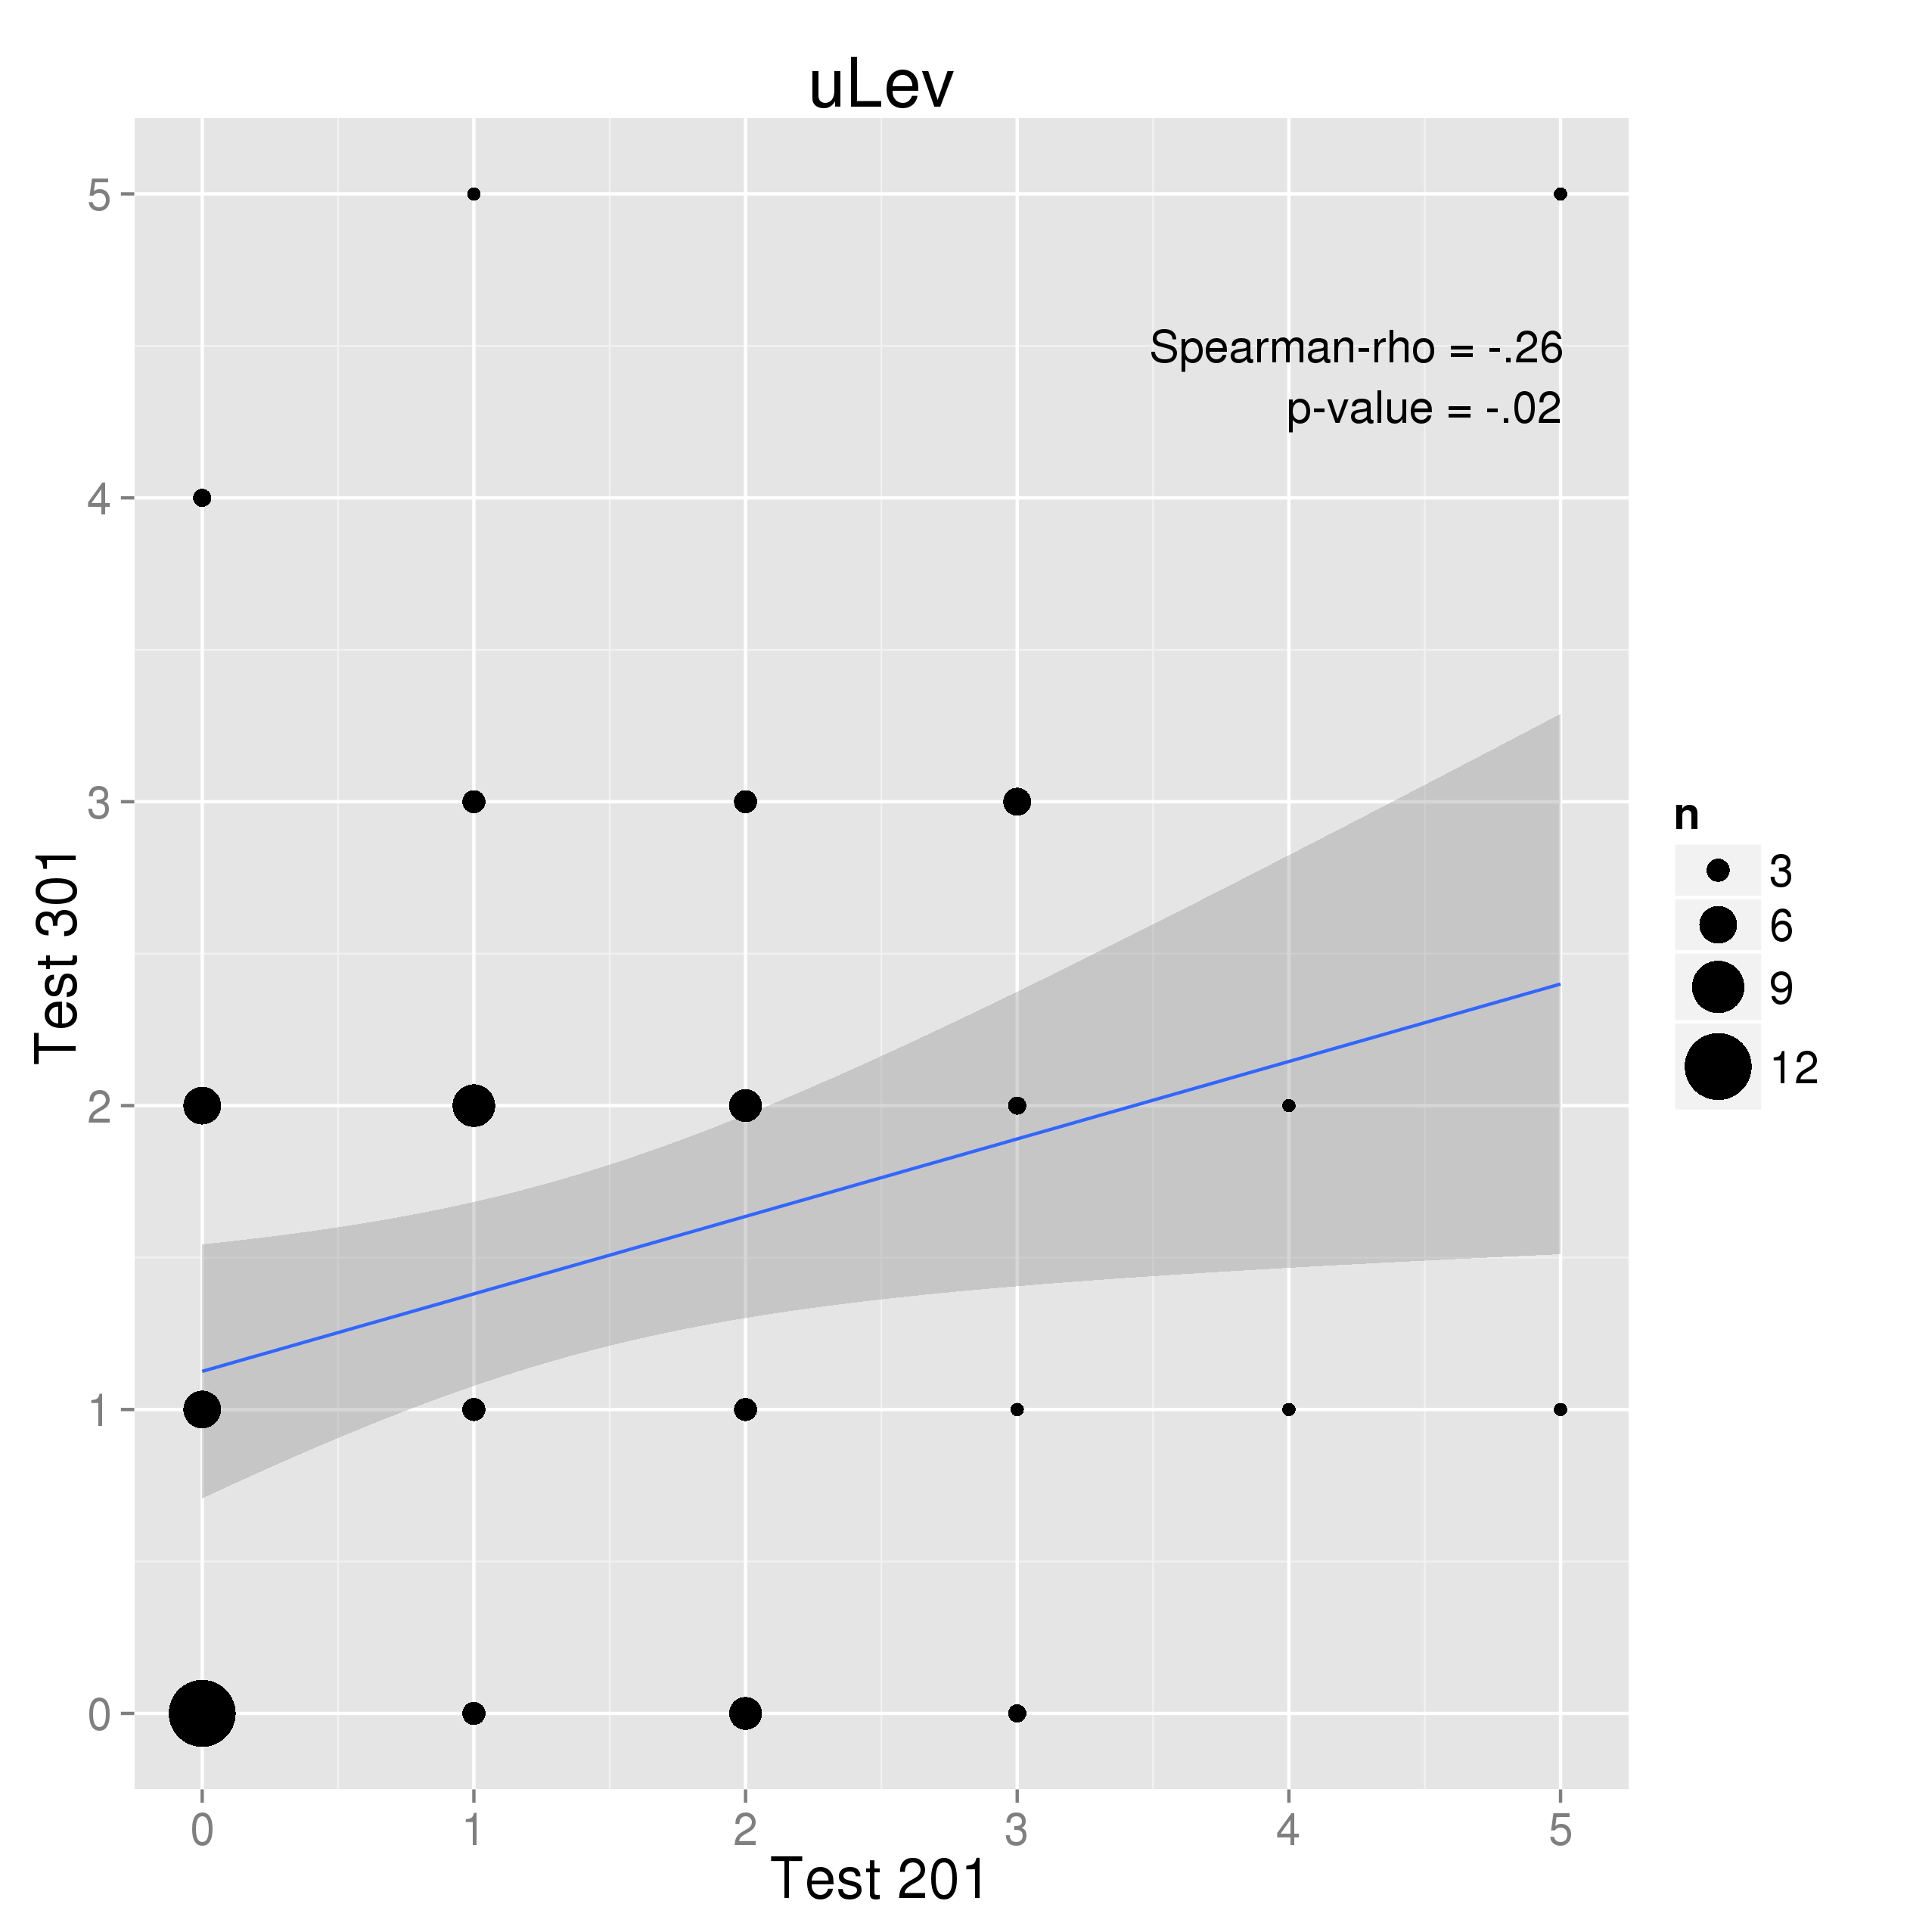
\includegraphics[width=1.0\linewidth]{graphics/cor201301u.png}
  \caption{Korrelation der unbedingten Niveau-Stufen zwischen Test 301 und 201.}
  \label{fig:cor201301k}
\end{subfigure}
\begin{subfigure}{0.49\textwidth}
  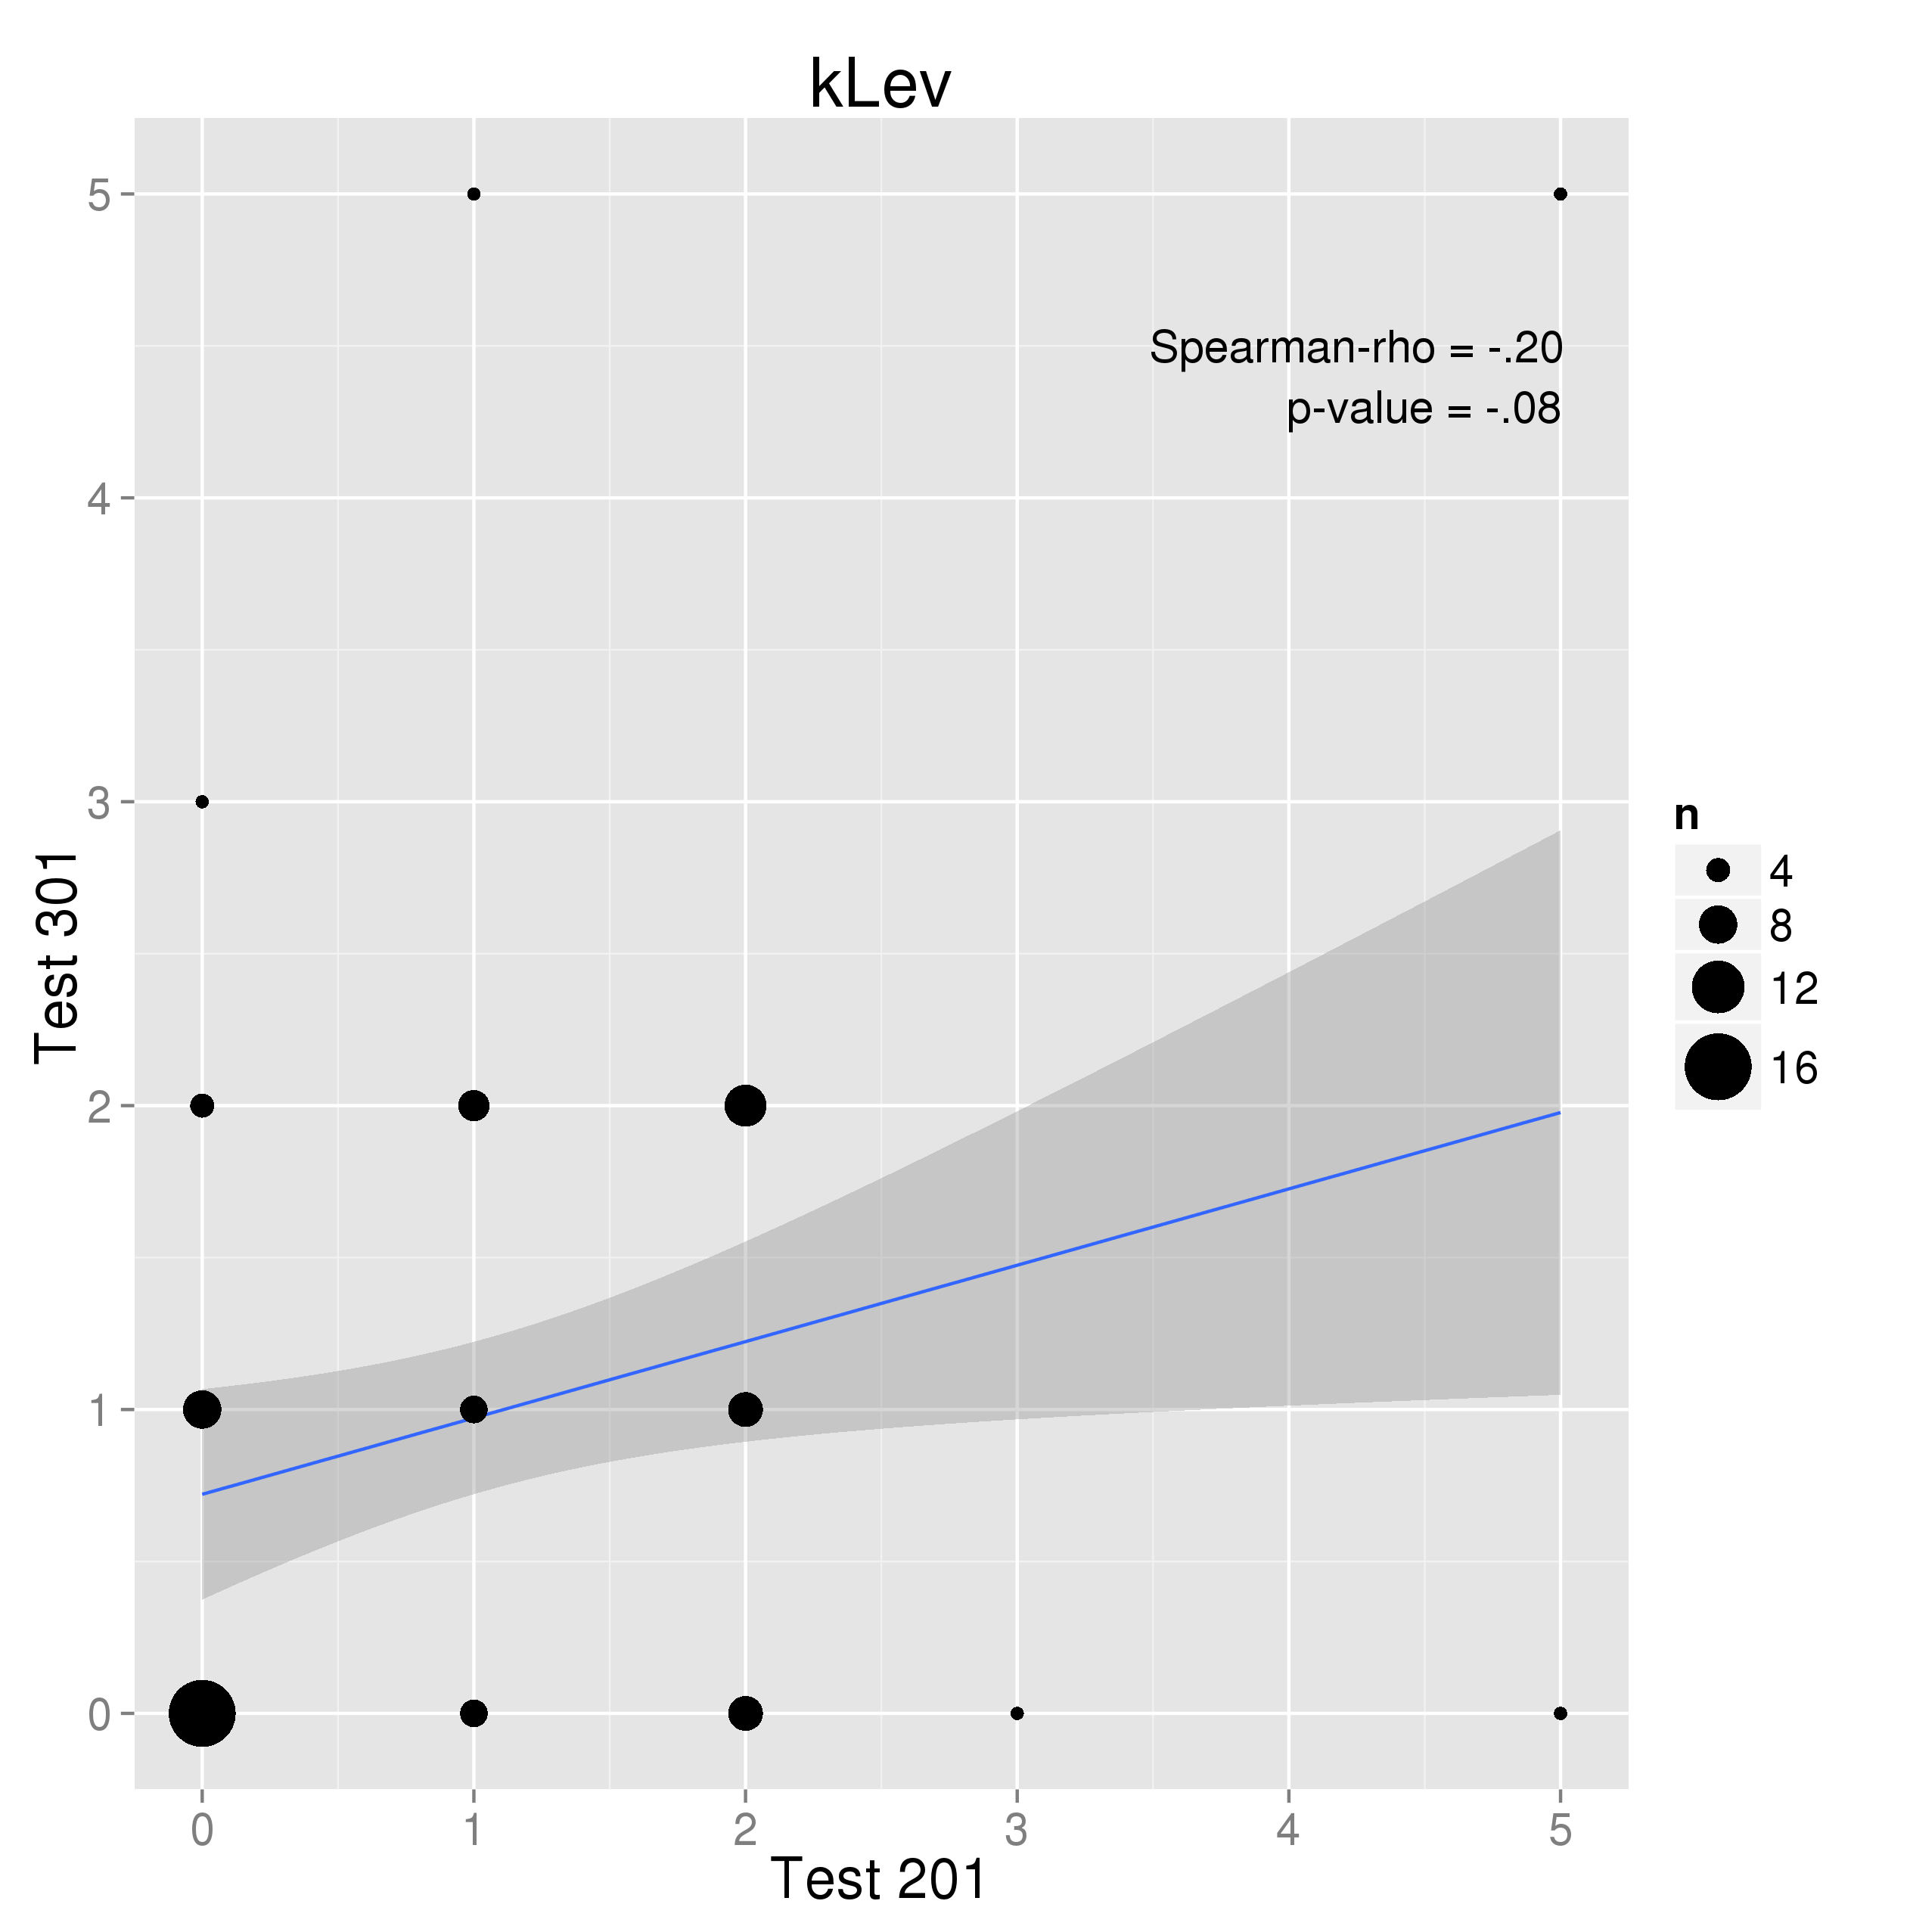
\includegraphics[width=1.0\linewidth]{graphics/cor201301k.png}
  \caption{Korrelation der bedingten Niveau-Stufen zwischen Test 301 und 201.}
  \label{fig:cor201301u}
\end{subfigure}
\end{figure}
\begin{figure}[htbp]
\ContinuedFloat % continue from previous page
\centering
\begin{subfigure}{0.49\textwidth}
  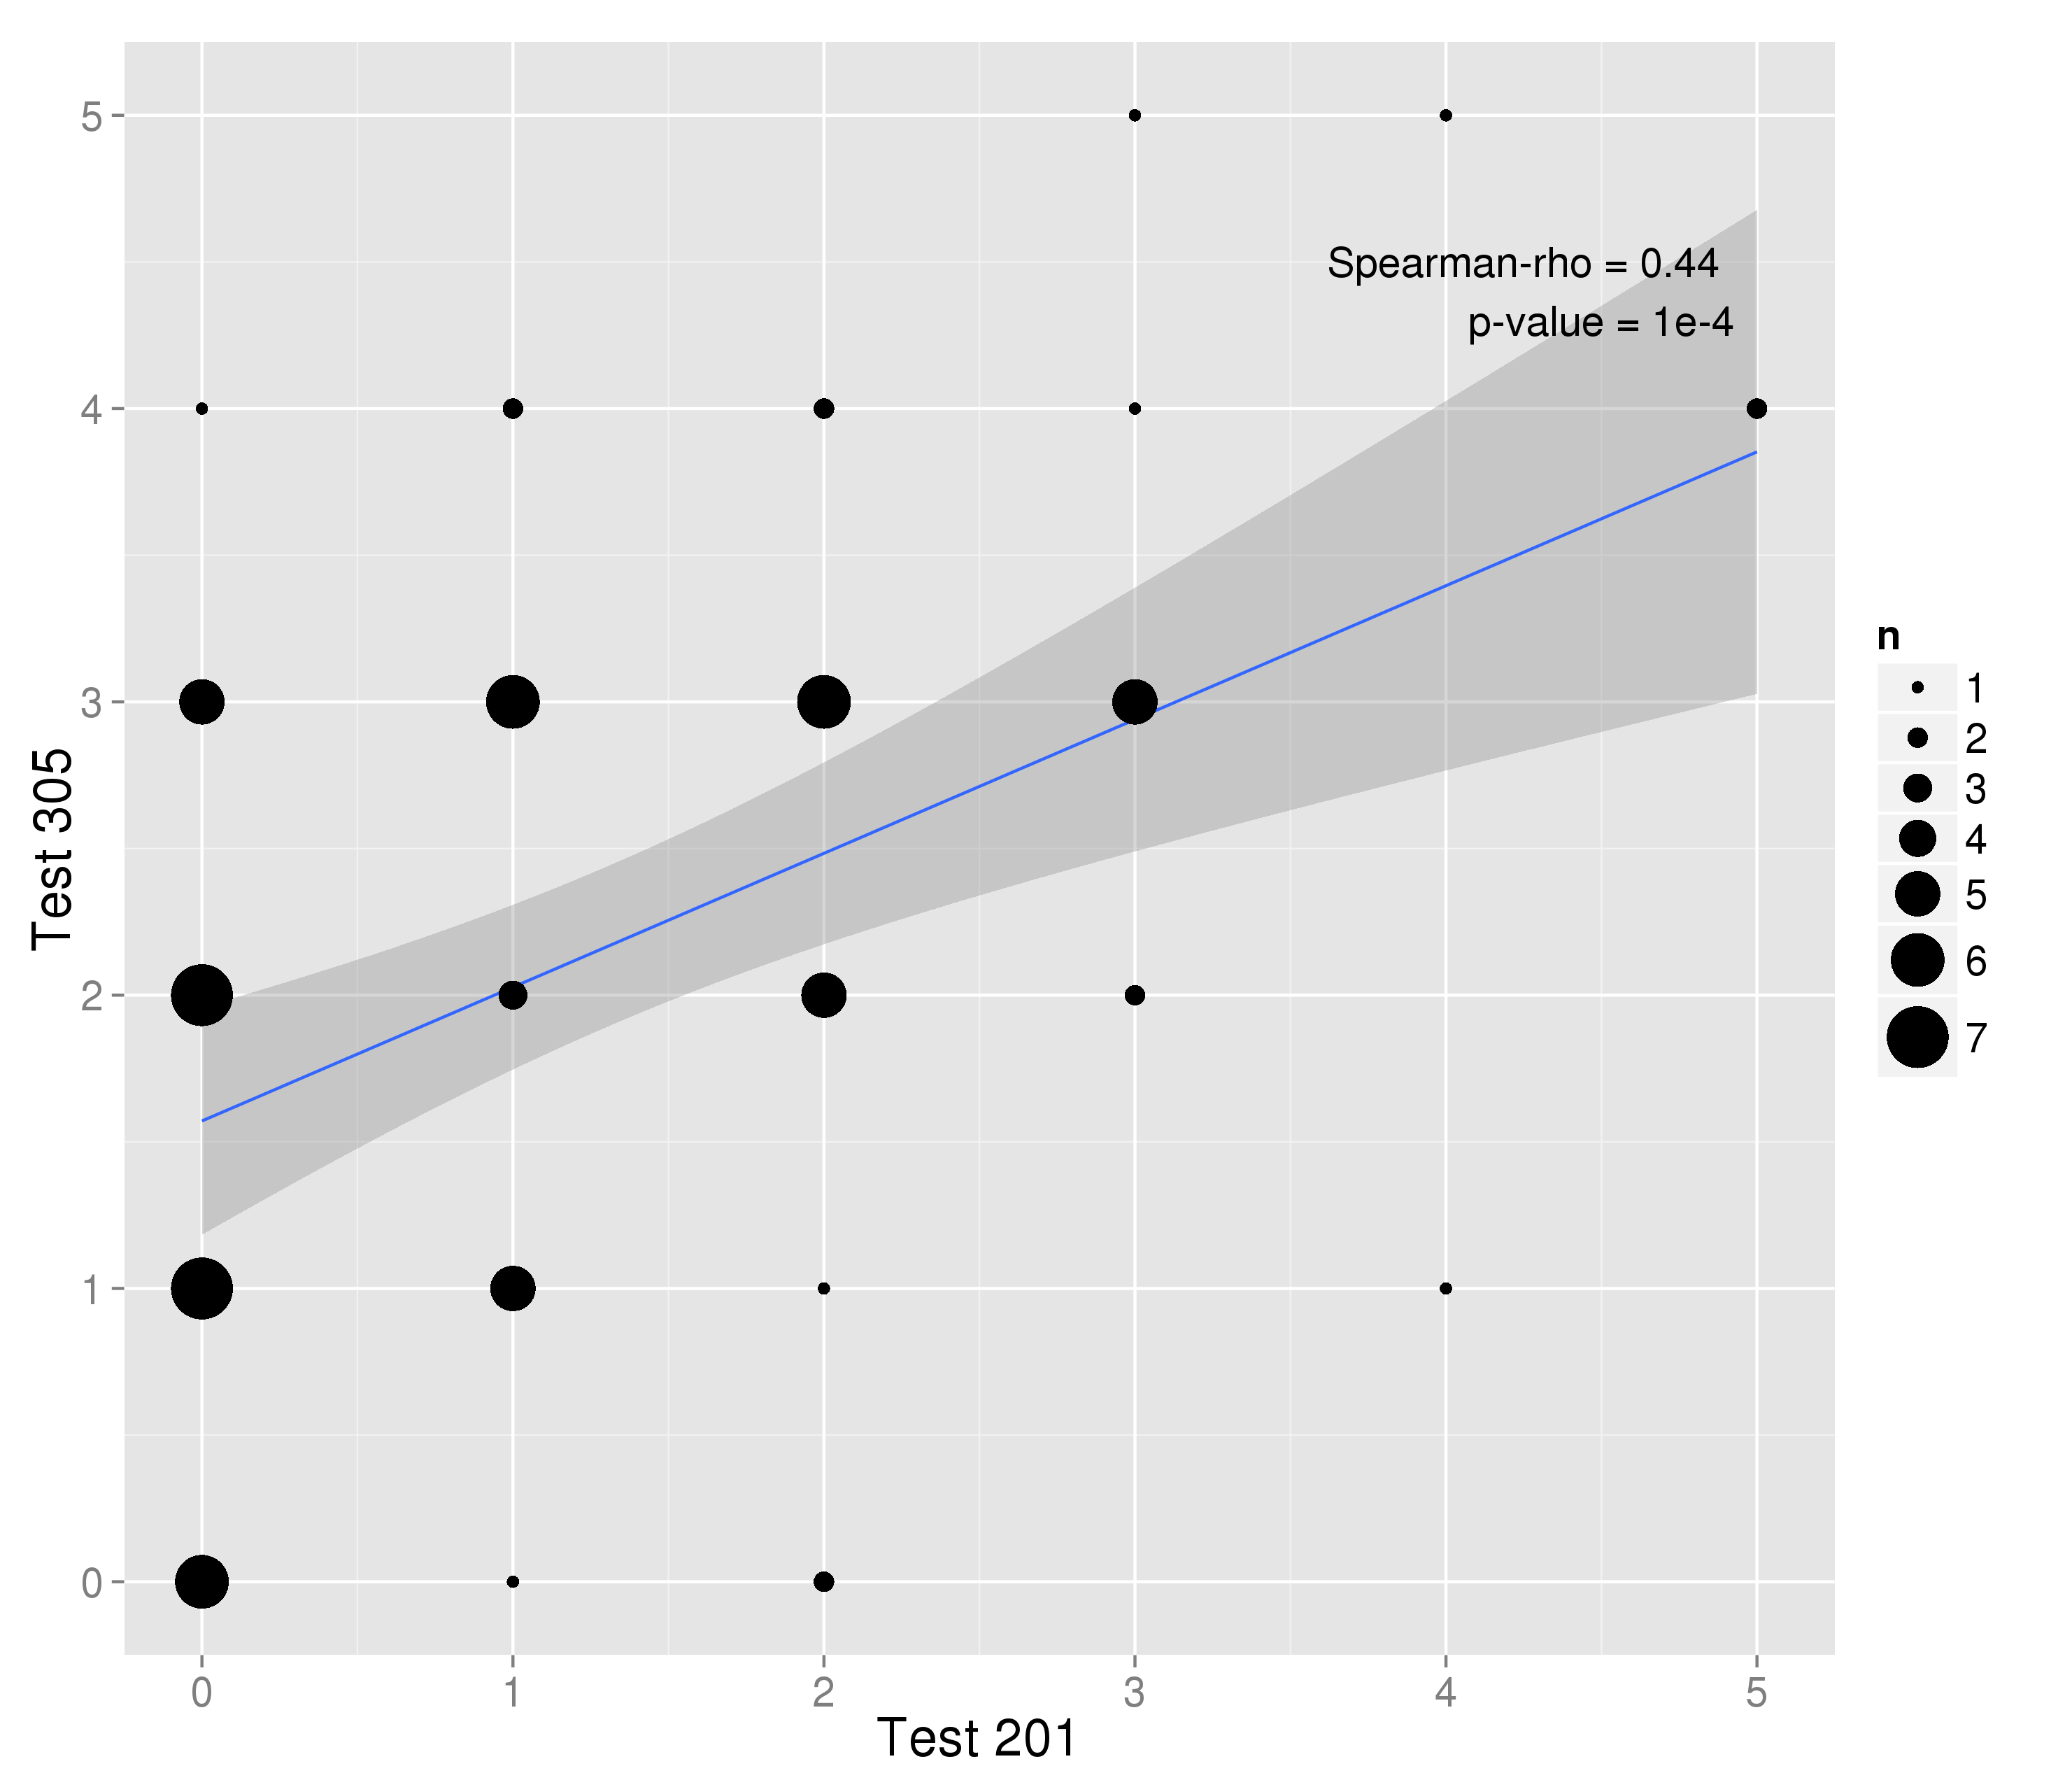
\includegraphics[width=1.0\linewidth]{graphics/cor201305u.png}
  \caption{Korrelation der unbedingten Niveau-Stufen zwischen Test 305 und 201.}
  \label{fig:cor201305k}
\end{subfigure}
\begin{subfigure}{0.49\textwidth}
  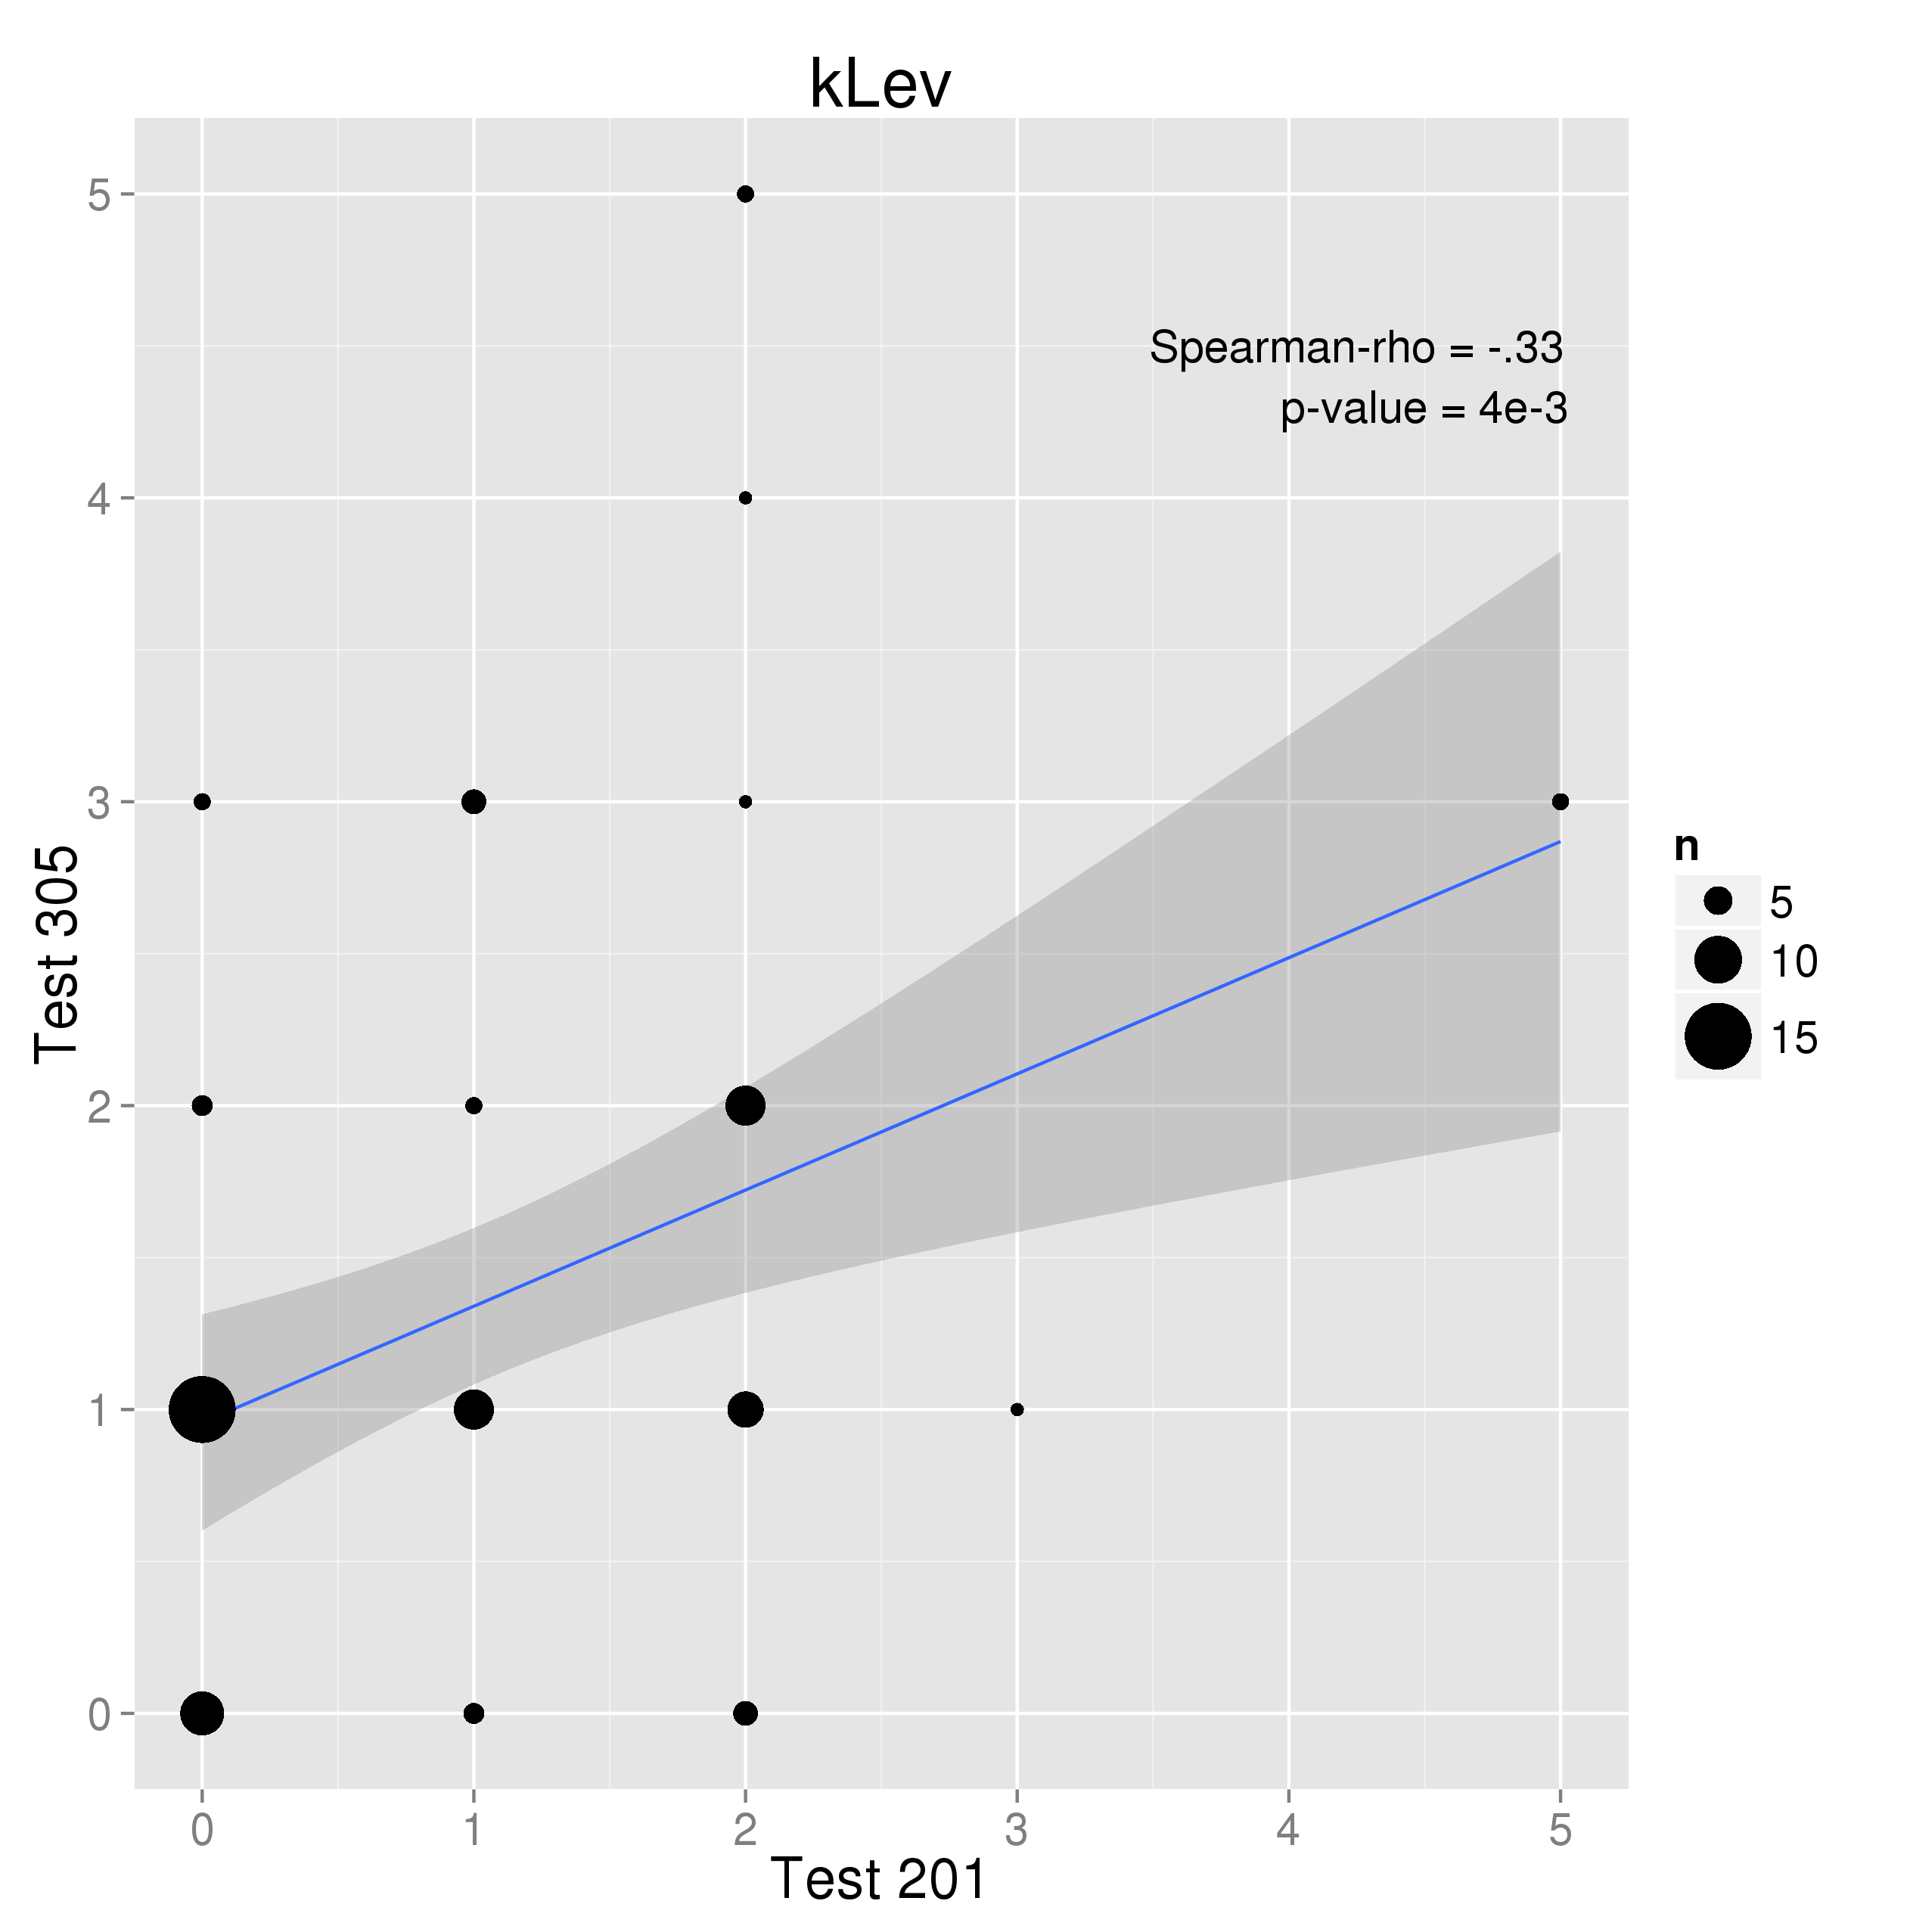
\includegraphics[width=1.0\linewidth]{graphics/cor201305k.png}
  \caption{Korrelation der bedingten Niveau-Stufen zwischen Test 305 und 201.}
  \label{fig:cor201305u}
\end{subfigure}
\end{figure}
\begin{figure}[htbp]
\ContinuedFloat % continue from previous page
\centering
\begin{subfigure}{0.49\textwidth}
  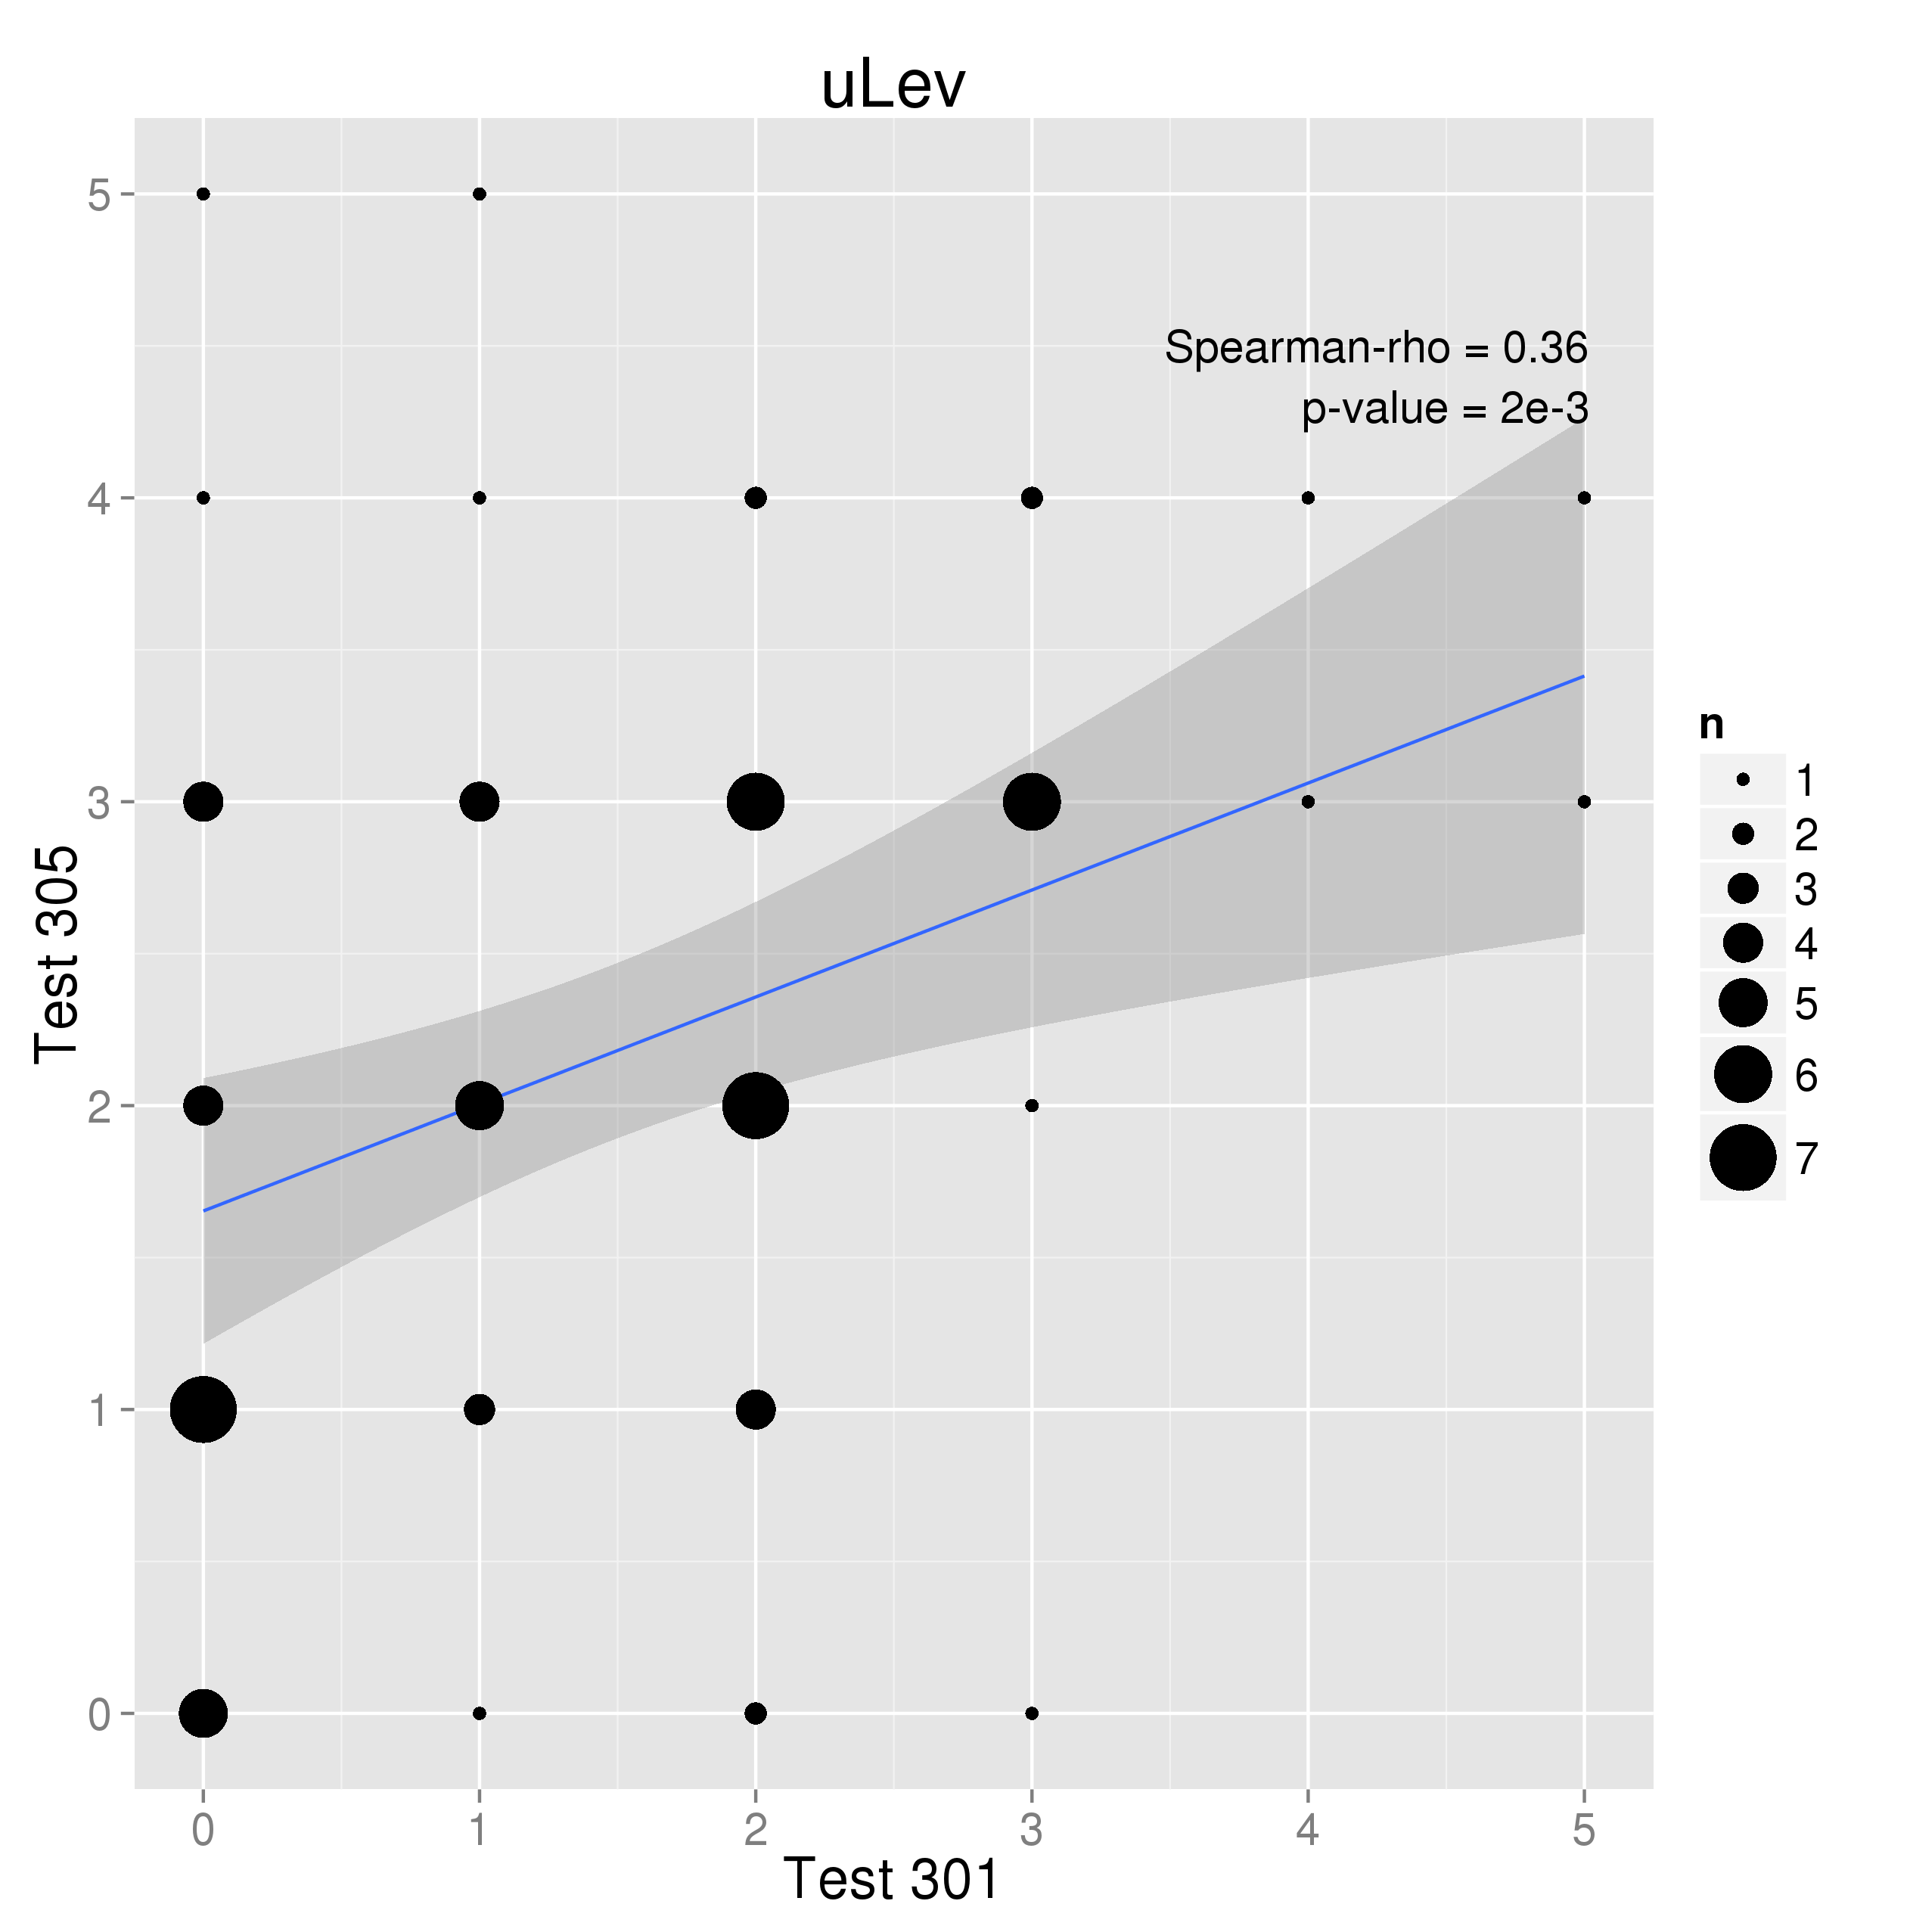
\includegraphics[width=1.0\linewidth]{graphics/cor301305u.png}
  \caption{Korrelation der unbedingten Niveau-Stufen zwischen Test 305 und 301.}
  \label{fig:cor301305k}
\end{subfigure}
\begin{subfigure}{0.49\textwidth}
  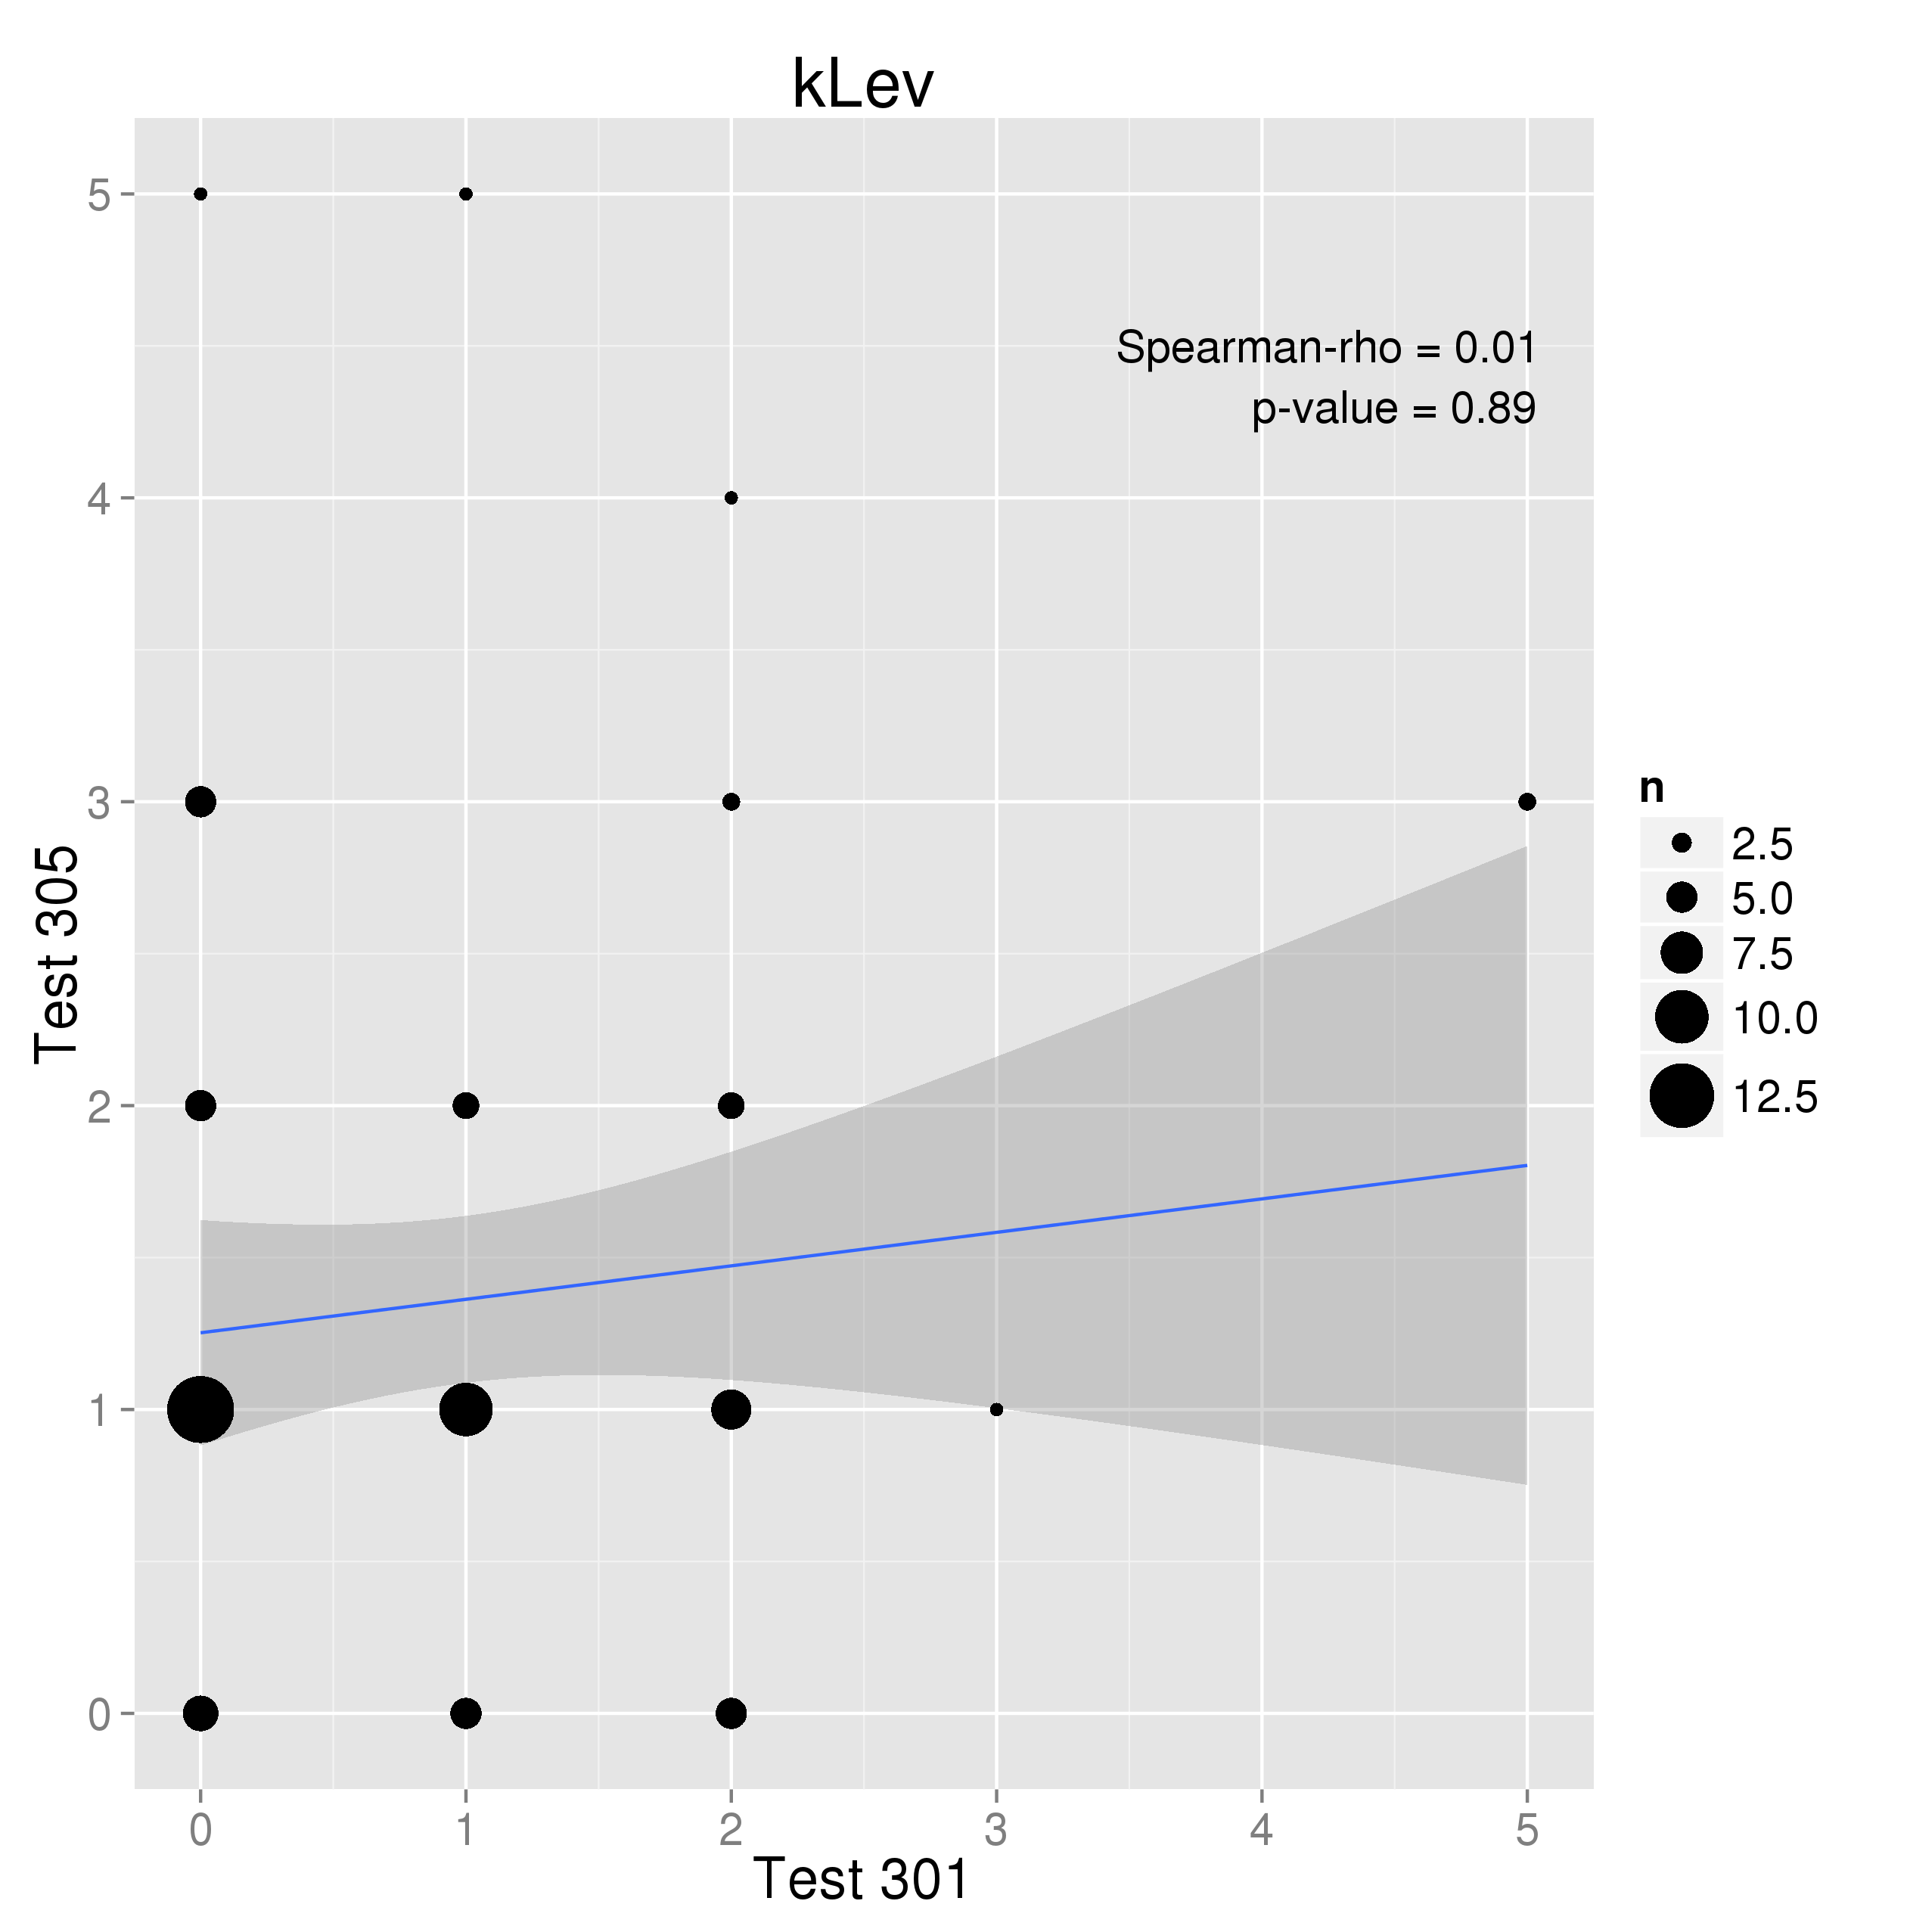
\includegraphics[width=1.0\linewidth]{graphics/cor301305k.png}
  \caption{Korrelation der bedingten Niveau-Stufen zwischen Test 305 und 301.}
  \label{fig:cor301305u}
\end{subfigure}

\caption{Korrelation zwischen den Niveau-Stufen der einzelnen Tests. Der Durchmesser der Punkte ist ein Mass für die Anzahl an Datenpunkten, welche an dieser Position liegen. Die blaue Gerade ist die lineare Regression der zugrunde liegenden Daten, der dunkel graue Bereich stellt das Vertrauensintervall (95\%) der linearen Regression dar. Zusätzlich sind noch Spearmans $rho$ und der p-Wert des Signifikanztests angegeben.}
\label{fig:corLev}
\end{figure}

\github{http://git.io/FnbD}

\clearpage
\section{Rasch-Analyse}

Als Probabilistische Test-Methode wurde das Rasch Modell verwendet. Der Grund für diese Methodik war, dass es sich bei der Kompetenz des skalenbasierten Messens um ein latentes Merkmal handelt. In anderen Worten die Kompetenz des skalenbaiserten Messens ist nicht direkt beobachtbar.

Es wurde zuerst folgendes Rasch Modell verwendet.

\begin{eqnarray}
P(U_{ij}=u_{ij}|\theta_i,\beta_j) = \frac{e^{u_{ij}(\theta_i-\beta_j)}}{1+e^{\theta_i-\beta_j}}
\end{eqnarray}

Wobei i=1,…,n die Zählvariable für eine Person ist und j=1,…,m die Zählvariable für eine Aufgabe darstellt. Die Variable $u_{ij} \in \{0,1\}$ die dichotome Antwort einer Person auf eine Frage ist. Die Variable $\beta_j$ beschreibt den Schwierigkeitsgrad einer Aufgabe und $\theta_j$ die latente Fähigkeit einer Person.

Bei der Item-Response-Theorie (Probabilistische Test-Methoden) wird angenommen , dass das Ergebnis einer Person nicht deterministisch ist, sondern zufällig sein kann. Daher soll mit dem Rasch Modell die Lösungswahrscheinlichkeit jeder Aufgabe $U_{ij}$ berechnet werden. Diese Lösungswahrscheinlichkeit hängt sowohl von der Fähigkeit der Person $\theta_j$ als auch von der Schwierigkeit der Aufgabe $\beta_i$ ab. Diese Lösungswahrscheinlichkeiten werden basierend auf den Testergebnissen $u_{ij}$ geschätzt.

\subsection{Parameter-Schätzung}
Für die Parameter-Schätzung gibt es verschieden Ansätze. Da die beste Methode von den Daten abhängig ist wurde in einem ersten Schritt das Rasch-Modell sowohl mit der bedingte Maximum"=Likelihood"=Schätzung, als auch mit der marginal Maximum"=Likelihood"=Schätzung getestet und die Resultate wurden verglichen. 

Bei der bedingten Maximum"=Likelihood"=Schätzung wird ein zweistufiges Vorgehen gewählt. Zuerst werden die Aufgaben-Parameter geschätzt ohne die Personen Parameter zu beachten. Erst in einem zweiten Schritt werden die Personen-Parameter geschätzt. Ein Problem dieser Methodik ist, dass Personenfertigkeiten von Personen, welche keine oder alle Aufgaben gelöst haben nicht geschätzt werden können \citep{Mair2007}.

In der marginalen Maximum"=Likelihood"=Schätzung wird angenommen, dass für die Personenfähigkeiten in der Stichprobe eine Normalverteilung vorliegt. Diese Annahme ist insbesondere dann problematisch, wenn nur eine Stichprobe der Gesamtbevölkerung verwendet wird \citep{Rizopoulos2006}.

Da beide Schätzungen für den vorliegenden Datensatz problematisch sein könnten, wurde das Rasch-Modell mit beiden Ansätzen durchgeführt und die Resultate verglichen. Das Ziel war dabei, den besseren Ansatz für den vorliegenden Datensatz zu finden, um mit diesem Ansatz die weiteren Analysen durchzuführen. Als Datensatz für diesen Vergleich wurden die 15 unbedingten Qualitätsstandards verwendet. Die Resultate sind in Abbildung \ref{fig:RaschVergleich} ersichtlich. Es gibt für diesen Datensatz keinerlei Unterschied in der Schätzung der Schwierigkeitsgrad der einzelnen Qualitätsstandards. 

Bei der Schätzung der Personen-Parametern $\theta$ konnte die bedingte Maximum"=Likelihood"=Schätzung alle 72 Personen-Fähigkeiten ohne Extrapolationen berechnen. Die marginalen Maximum"=Likelihood"=Schätzung konnte jedoch nur die Personen"=Fähigkeiten von 64 Personen berechnen. Daher wird in der weiteren Arbeit für alle Rasch Modelle jeweils der bedingten Maximum-Likelihood-Schätzer verwendet.


\begin{figure}[htbp]

\centering
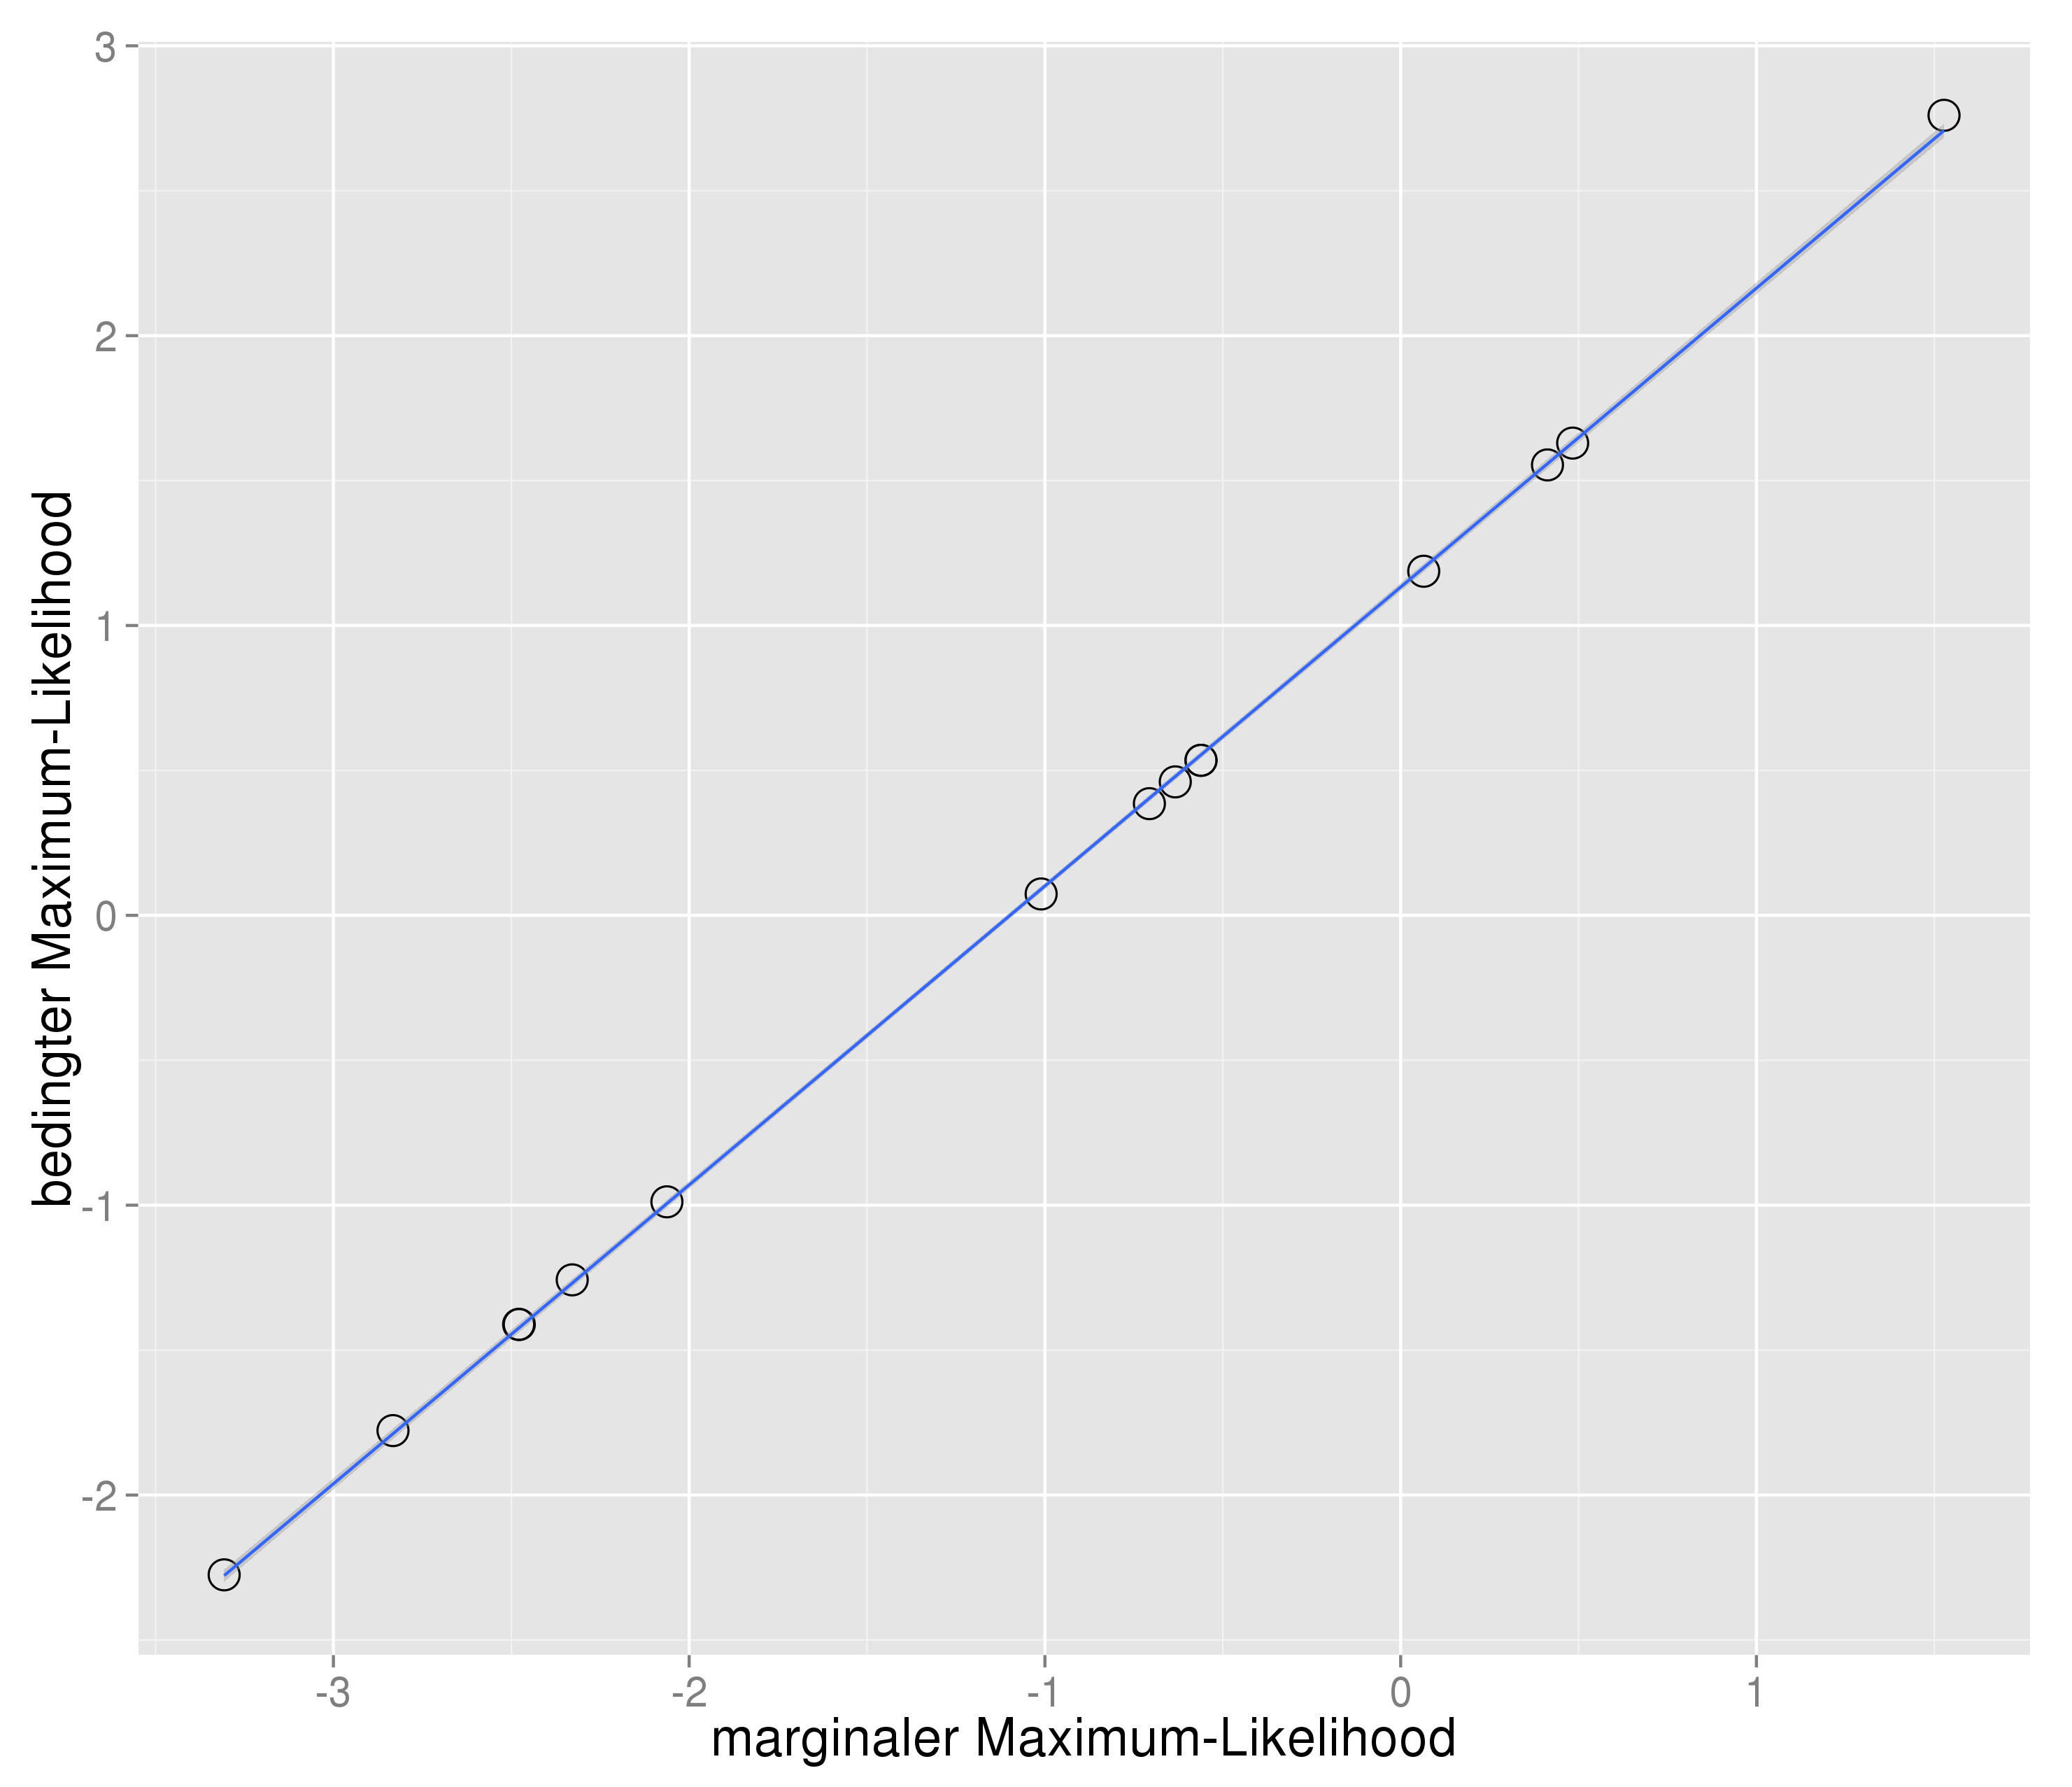
\includegraphics[width=0.6\linewidth]{graphics/RaschVergleich.png}
\caption{Vergleich des Rasch Modells mit der bedingten Maximum"=Likelihood"=Schätzung und der marginalen Maximum"=Likelihood"=Schätzung. Da alle Punkte auf einer Geraden liegen, gibt es keinen Unterschied zwischen den unterschiedlichen Schätzmethoden für den vorliegenden Datensatz der 15 unbedingten Qualitätsstandards.  }
\label{fig:RaschVergleich}
\end{figure}


Es gibt noch weitere Parameter Schätzer wie den Bayesianischen Ansatz, welcher Markov-Chain-Monte-Carlo Methoden verwendet. Dieser trifft jedoch auch Annahmen über die Verteilung der Personen Parameter \citep[siehe Kapitel 3]{Fischer1995}. Die Annahmen decken sich daher mit dem marginalen Maximum-Likelihood Schätzer. 


\github{http://git.io/FRxZ}


\subsection{Modellkontrolle des Rasch-Modells}

Um das Rasch Modell zu Validieren wurde das Modell mit Hilfe des Andersens Likelihood-Quotienten Test validiert. Für alle 15 Qualitätsstufen führte dies zu Problemen und der Test konnte nicht durchgeführt werden. Nachdem die Qualitätsstufen vier und fünf entfernt wurden, konnte das reduzierte Modell validiert werden. Als Splitkriterium wurde der Mittelwert der Personen-Randsummen verwendet. 

Der p-Wert des Andersens Likelihood-Quotienten Test beträgt $p=0.14$. Daher liegt jetzt keine signifikante Modellverletzung vor, die Aufgaben Parameter unterscheiden sich nicht signifikant für Personen mit niedrigen und hohen Randsummen. In der Grafik \ref{fig:RaschKontrolle} sind die Resultate des Tests grafisch dargestellt. Es ist ersichtlich, dass keine Aufgabe das Modell verletzt, da die 95\%-Konfidenz-Regionen alle die Diagonale berühren.


\begin{figure}[htbp]

\centering
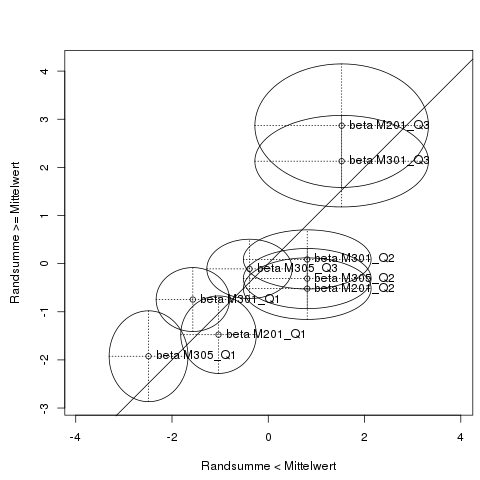
\includegraphics[width=0.8\linewidth]{graphics/GOFQ.png}
\caption{Modellkontrolle des Rasch-Modells: kein Qualitätsstandard hat eine signifikante Abweichung von der Diagonalen, daher gibt es keine signifikanten Unterschiede für Personen mit niedrigen und hohen Randsummen in den Qualitätsstandard. }
\label{fig:RaschKontrolle}
\end{figure}

Zusätzlich wurden die Qualitätsstandards mit dem Wald-Test überprüft. Damit können Qualitätsstandard, welche einen signifikanten Unterschied habe, identifiziert werden. In Tabelle \ref{tab:WaldTest} befinden sich die p-Werte des Wald-Test für die einzelnen Qualitätsstandards.

\begin{table}[htbp]
  \centering
\begin{tabular}{@{}lllllllllll@{}}
\toprule
 \multicolumn{3}{c}{Test 201} &&  \multicolumn{3}{c}{Test 301}&&  \multicolumn{3}{c}{Test 305}\\ 
    \cmidrule{1-3}\cmidrule{5-7}\cmidrule{9-11}
 Q1 & Q2 & Q3 && Q1 & Q2 & Q3 && Q1 & Q2 & Q3  \\ 
\midrule
  0.44 & 0.08 & 0.24 && 0.11 & 0.33 & 0.56 && 0.38 & 0.14 & 0.61   \\ 

\bottomrule
\end{tabular} 
  \caption{p-Werte des Wald-Tests für die Qualitätsstandards, mit dem Mittelwert der Personen-Randsummen als Splitkriterium. Keine dieser p-Werte liegt unter halb von $0.05$ daher gibt es keine signifikanten Unterschiede in den Qualitätsstandards }
  \label{tab:WaldTest}
\end{table}

\github{http://git.io/FE3m}

\subsection{Unterschied in den Schwierigkeiten der Qualitätsstandards}

Nachdem das Modell kontrolliert wurde soll nun überprüft werden ob es einen Unterschied in den Qualitätsstandards zwischen den einzelnen Test gibt.


  
 \begin{figure}[htp]
 \centering
 \begin{subfigure}{0.49\textwidth}
   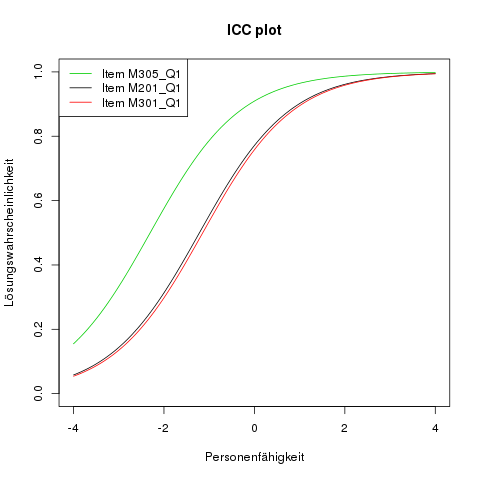
\includegraphics[width=1.0\linewidth]{graphics/ICCQ1.png}
   \caption{ICC Plot für Qualitätsstandard 1}
   \label{fig:ICCQ1}
 \end{subfigure}
 \begin{subfigure}{0.49\textwidth}
   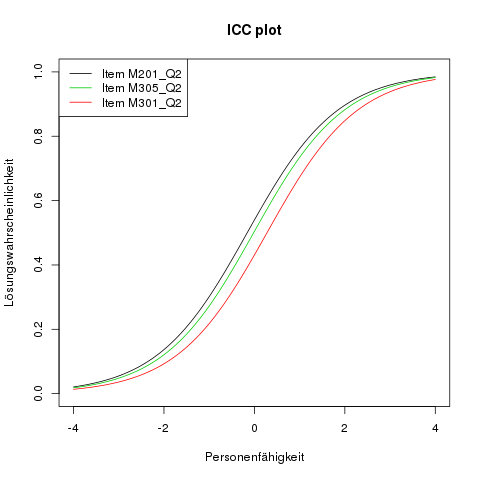
\includegraphics[width=1.0\linewidth]{graphics/ICCQ2.png}
   \caption{ICC Plot für Qualitätsstandard 2}
   \label{fig:ICCQ2}
 \end{subfigure}
 \end{figure}
 \begin{figure}[htbp]
 \ContinuedFloat % continue from previous page
 \centering
 \begin{subfigure}{0.49\textwidth}
   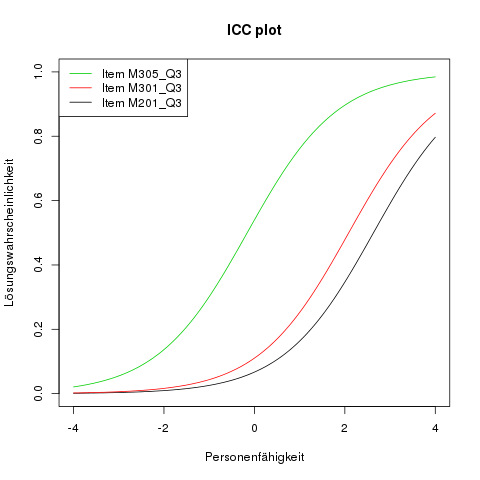
\includegraphics[width=1.0\linewidth]{graphics/ICCQ3.png}
   \caption{ICC Plot für Qualitätsstandard 3}
   \label{fig:ICCQ3}
 \end{subfigure}
 \begin{subfigure}{0.49\textwidth}
   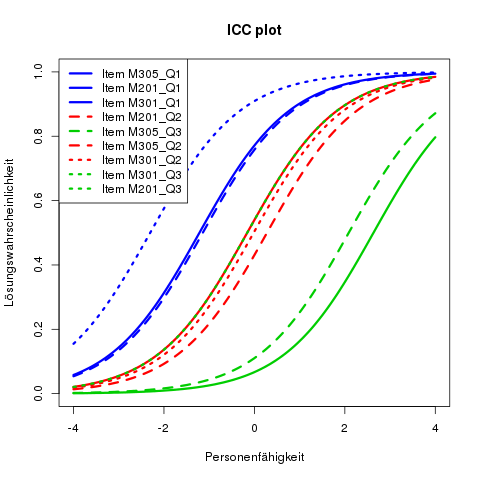
\includegraphics[width=1.0\linewidth]{graphics/ICCQ123.png}
   \caption{ICC Plot für Qualitätsstandard 1,2 und 3}
   \label{fig:ICCQ123}
 \end{subfigure}
 
 \caption{Aufgabencharakteristische Kurven für die Qualitätsstandards 1,2 und 3 für alle drei Tests.}
 \label{fig:corLevRasch}
 \end{figure}
 
 \begin{figure}[htbp]
 
 \centering
 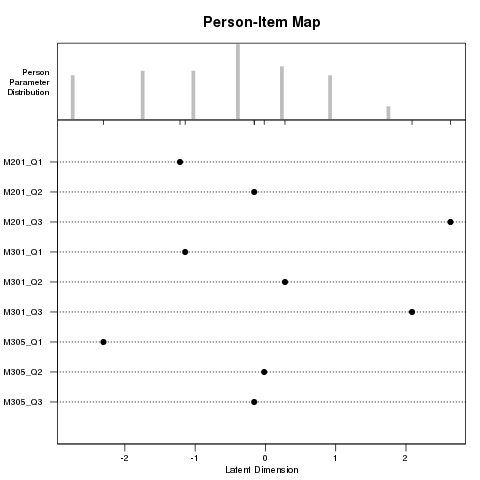
\includegraphics[width=0.8\linewidth]{graphics/PersonItemMap.png}
 \caption{Person-Item-Map auf welcher die Verteilung der Personen basierend auf der latenten Skala ersichtlich ist und die Lage der Aufgaben-Parameter auf der latenten Skala. Anhand dieser Darstellung kann man sehen, dass z.B. der Qualitätsstandard 1 im Test 201 und im Test 301 einen sehr ähnlichen Schwierigkeitsgrad besitzen. }
 \label{fig:PersonItemMapQ}
 \end{figure}
 
 In Tabelle \ref{tab:betaQ} finden sich die Aufgaben-Parameter $\beta_j$ der einzelnen Qualitätsstandards.
 
 \begin{table}[htbp]
   \centering
 \begin{tabular}{@{}lllllllllll@{}}
 \toprule
  \multicolumn{3}{c}{Test 201} &&  \multicolumn{3}{c}{Test 301}&&  \multicolumn{3}{c}{Test 305}\\ 
   \cmidrule{1-3}\cmidrule{5-7}\cmidrule{9-11}
  Q1 & Q2 & Q3 && Q1 & Q2 & Q3 && Q1 & Q2 & Q3  \\ 
 \midrule
   1.215 & 0.159 & -2.633 && 1.142 & -0.278 & -2.086 && 2.305 & 0.017 & 0.159   \\ 
 
 \bottomrule
 \end{tabular} 
   \caption{Aufgaben-Parameter $\beta_j$ für die einzelnen Qualitätsstandards. }
   \label{tab:betaQ}
 \end{table}
 
 Mit den so gewonnen Aufgaben-Parametern $\beta_j$ wurde nun die Korrelation zwischen den einzelnen Test berechnet. Da mit dem bisherigen Rasch Modell der Personen-Parameter $\theta_i$ über alle drei Tests identisch ist, sollten sich die Schwierigkeitsgerade der einzelnen Qualitätsstufen in den Tests sich nicht unterscheiden. Die Ergebnisse dieser Analyse sind im der Darstellung \ref{fig:corTestQ} und in Tabelle \ref{tab:corTestQ} angegeben. Wichtig dabei ist, dass der Stichproben Umfang mit 3 sehr gering ist. 
 
 
  \begin{figure}[htp]
  \centering
  \begin{subfigure}{0.32\textwidth}
    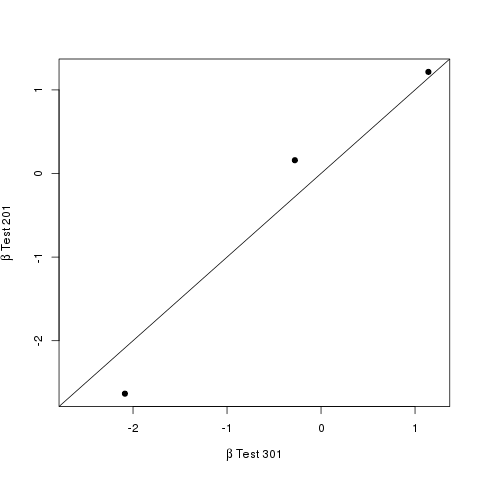
\includegraphics[width=1.0\linewidth]{graphics/GOF201301.png}
    \caption{Vergleich der Aufgaben-Parameter $\beta_j$ zwischen Test 201 und 301.}
    \label{fig:cor201301}
  \end{subfigure}
  \begin{subfigure}{0.32\textwidth}
    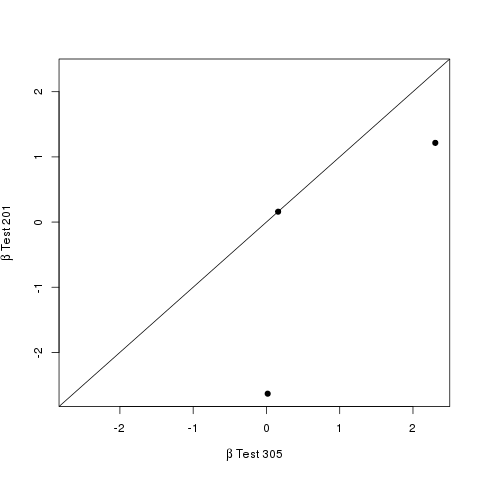
\includegraphics[width=1.0\linewidth]{graphics/GOF201305.png}
    \caption{Vergleich der Aufgaben-Parameter $\beta_j$ zwischen Test 201 und 305.}
    \label{fig:cor201305}
  \end{subfigure}
  \begin{subfigure}{0.32\textwidth}
    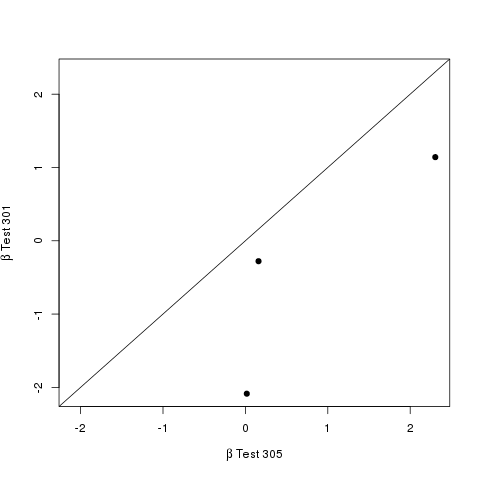
\includegraphics[width=1.0\linewidth]{graphics/GOF301305.png}
    \caption{Vergleich der Aufgaben-Parameter $\beta_j$ zwischen Test 301 und 305.}
    \label{fig:cor301305}
  \end{subfigure}
  
  \caption{Vergleich der Aufgaben Parameter zwischen den einzelnen Test. Wenn die Schwierigkeiten der Qualitätsstandards übereinstimmen würden, müssten alle Punkte auf der Winke-Halbierenden liegen.}
  \label{fig:corTestQ}
  \end{figure}
 
  \begin{table}[htbp]
    \centering
  \begin{tabular}{@{}llllllll@{}}
  \toprule
   \multicolumn{2}{c}{201 vs 301} &&  \multicolumn{2}{c}{201 vs 305}&&  \multicolumn{2}{c}{301 vs 305}\\ 
      \cmidrule{1-2} \cmidrule{4-5} \cmidrule{7-8}   
   p-Wert & ks && p-Wert & ks && p-Wert & ks  \\ 
  \midrule
    1.00 & 0.33 && 1.00 & 0.33 && 0.60 & 0.67  \\ 
  
  \bottomrule
  \end{tabular} 
    \caption{Resultate des Kolmogorow-Smirnow-Test für die Übereinstimmung der Schwierigkeiten der Qualitätsstandards. Wobei ks die Test-Statistik des Kolmogorow-Smirnow-Test ist.}
    \label{tab:corTestQ}
  \end{table}
  
  \github{http://git.io/FVZt}
  
  
\subsection{Unterschied in den latenten Personen-Fähigkeiten}

Nachdem in einem ersten Schritt die Schwierigkeit der Qualitätsstandards untersucht wurde und festgestellt wurde, dass keine signifikante Unterschiede in den Schwierigkeitsgeraden zwischen den einzelnen Tests existieren, wurde nun ein neues Rasch-Modell entwickelt.

Es werden jetzt drei Rasch Modelle gebildet, bei denen jeder Test und dessen Qualitätsstandards 1-3 in einem Modell kombiniert wurden. Aus den drei Modellen wurden die Personen-Fähigkeiten berechnet und dann mit dem Kolmogorow-Smirnow-Test auf den Goodness of fit überprüft. Dabei wurden Personen Parameter, welche Aufgrund des bedingten Maximum-Likelihood Schätzers nicht berechnet werden konnten aus den Daten heraus gefiltert. Wichtig hierbei ist jedoch, dass diese drei Rasch Modelle aufgrund der Probleme mit dem Parameter Schätzer, nicht evaluiert werden konnten, da die Datensätze zu gering waren. Um diesen Vergleich sinnvoll durchzuführen bräuchte es einen neuen besseren Schätzer. Der marginal Maximum-Likelihood Schätzer konnte deutlich weniger Personen Parameter schätzen, als der bedinge Maximum-Likelihood Schätzer. 

Die Ergebnisse der Test befinden sich in den Darstellungen \ref{fig:GOFP} und die wichtigesten Test Parameter in Tabelle \ref{tab:GOFP}.
   \begin{table}[htbp]
     \centering
   \begin{tabular}{@{}lllllllllll@{}}
   \toprule
    \multicolumn{3}{c}{201 vs 301} &&  \multicolumn{3}{c}{201 vs 305}&&  \multicolumn{3}{c}{301 vs 305}\\ 
       \cmidrule{1-3}\cmidrule{5-7}\cmidrule{9-11}
    p-Wert & ks & n && p-Wert & ks & n && p-Wert & ks & n \\ 
   \midrule
     2e-3 & 0.45 & 33&& 1e-6 & 0.62 & 37 && 1e-3 & 0.60 & 20  \\ 
   
   \bottomrule
   \end{tabular} 
     \caption{Resultate des Kolmogorow-Smirnow-Test für die Übereinstimmung der Personen-Parameter zwischen den drei Tests. Wobei ks die Test-Statistik des Kolmogorow-Smirnow-Test ist. Mit $n$ wird die Anzahl an Personenparametern angegeben, welche für den Test verwendet werden konnten. }
     \label{tab:GOFP}
   \end{table}
   

   
 \begin{figure}[htp]
 \centering
 \begin{subfigure}{0.49\textwidth}
   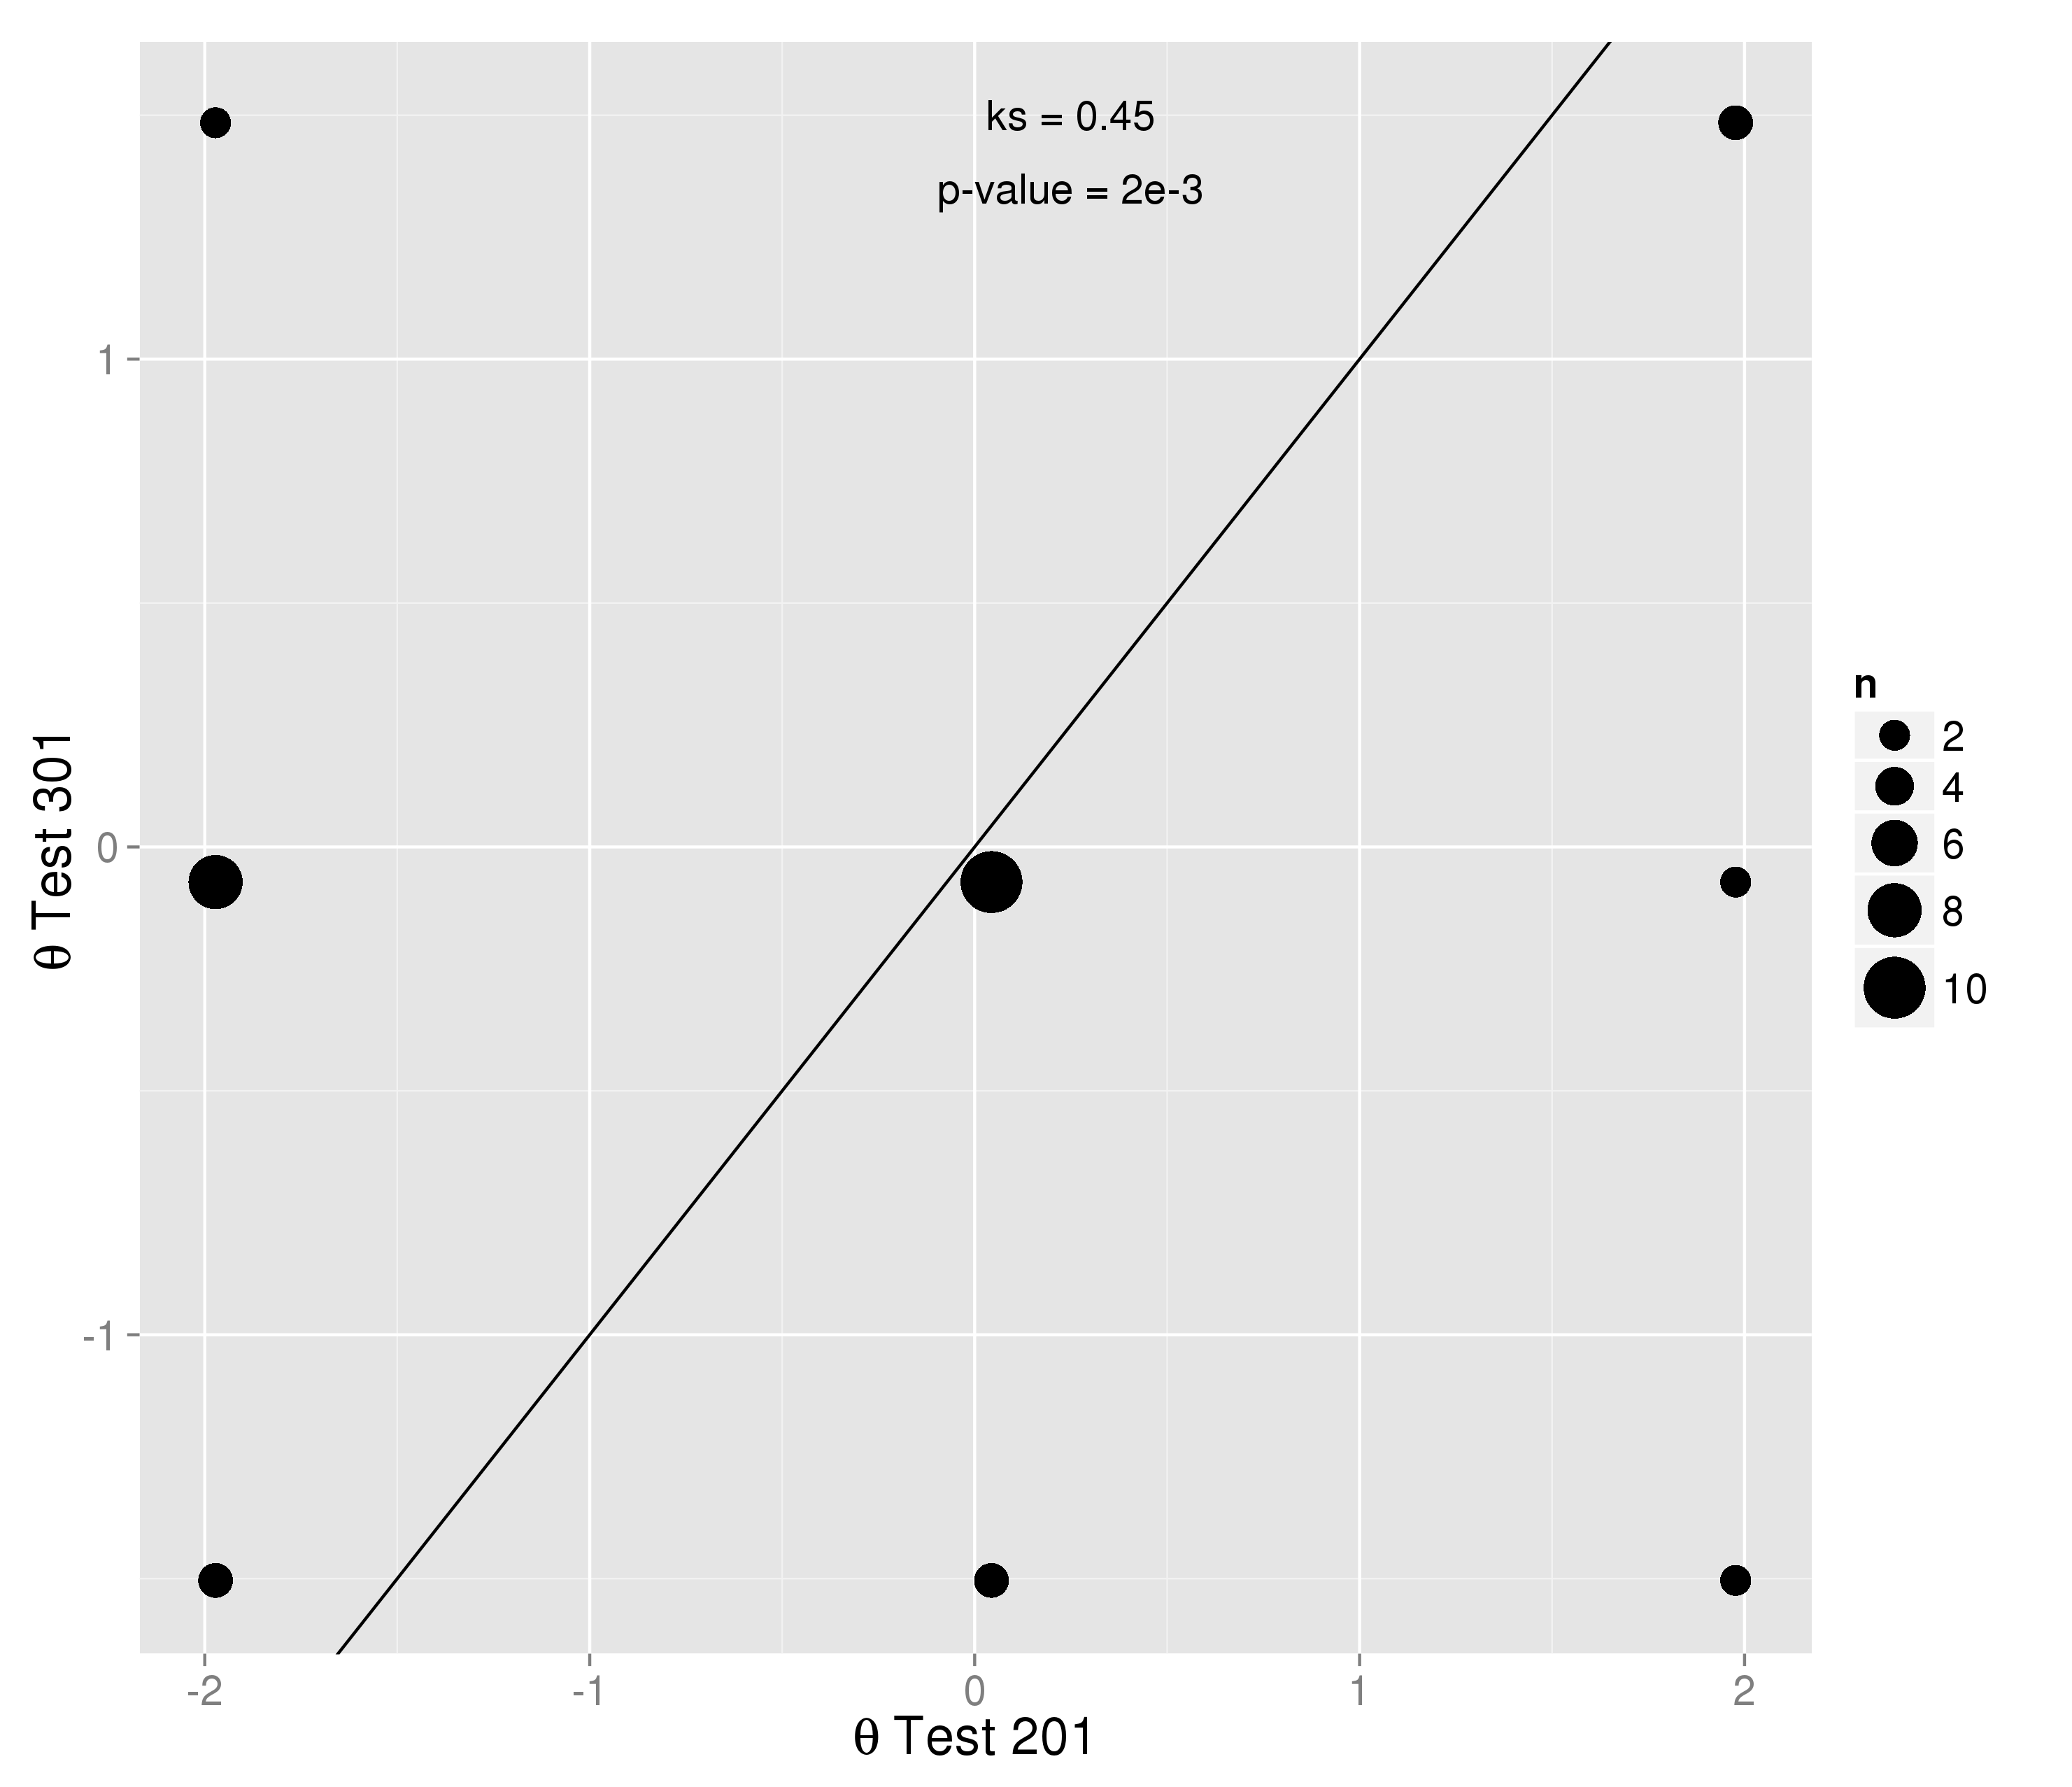
\includegraphics[width=1.0\linewidth]{graphics/GOF201301Pers.png}
   \caption{Vergleich der Personen-Parameter $\theta_i$ zwischen Test 201 und 301.}
   \label{fig:GOF201301P}
 \end{subfigure}
 \begin{subfigure}{0.49\textwidth}
   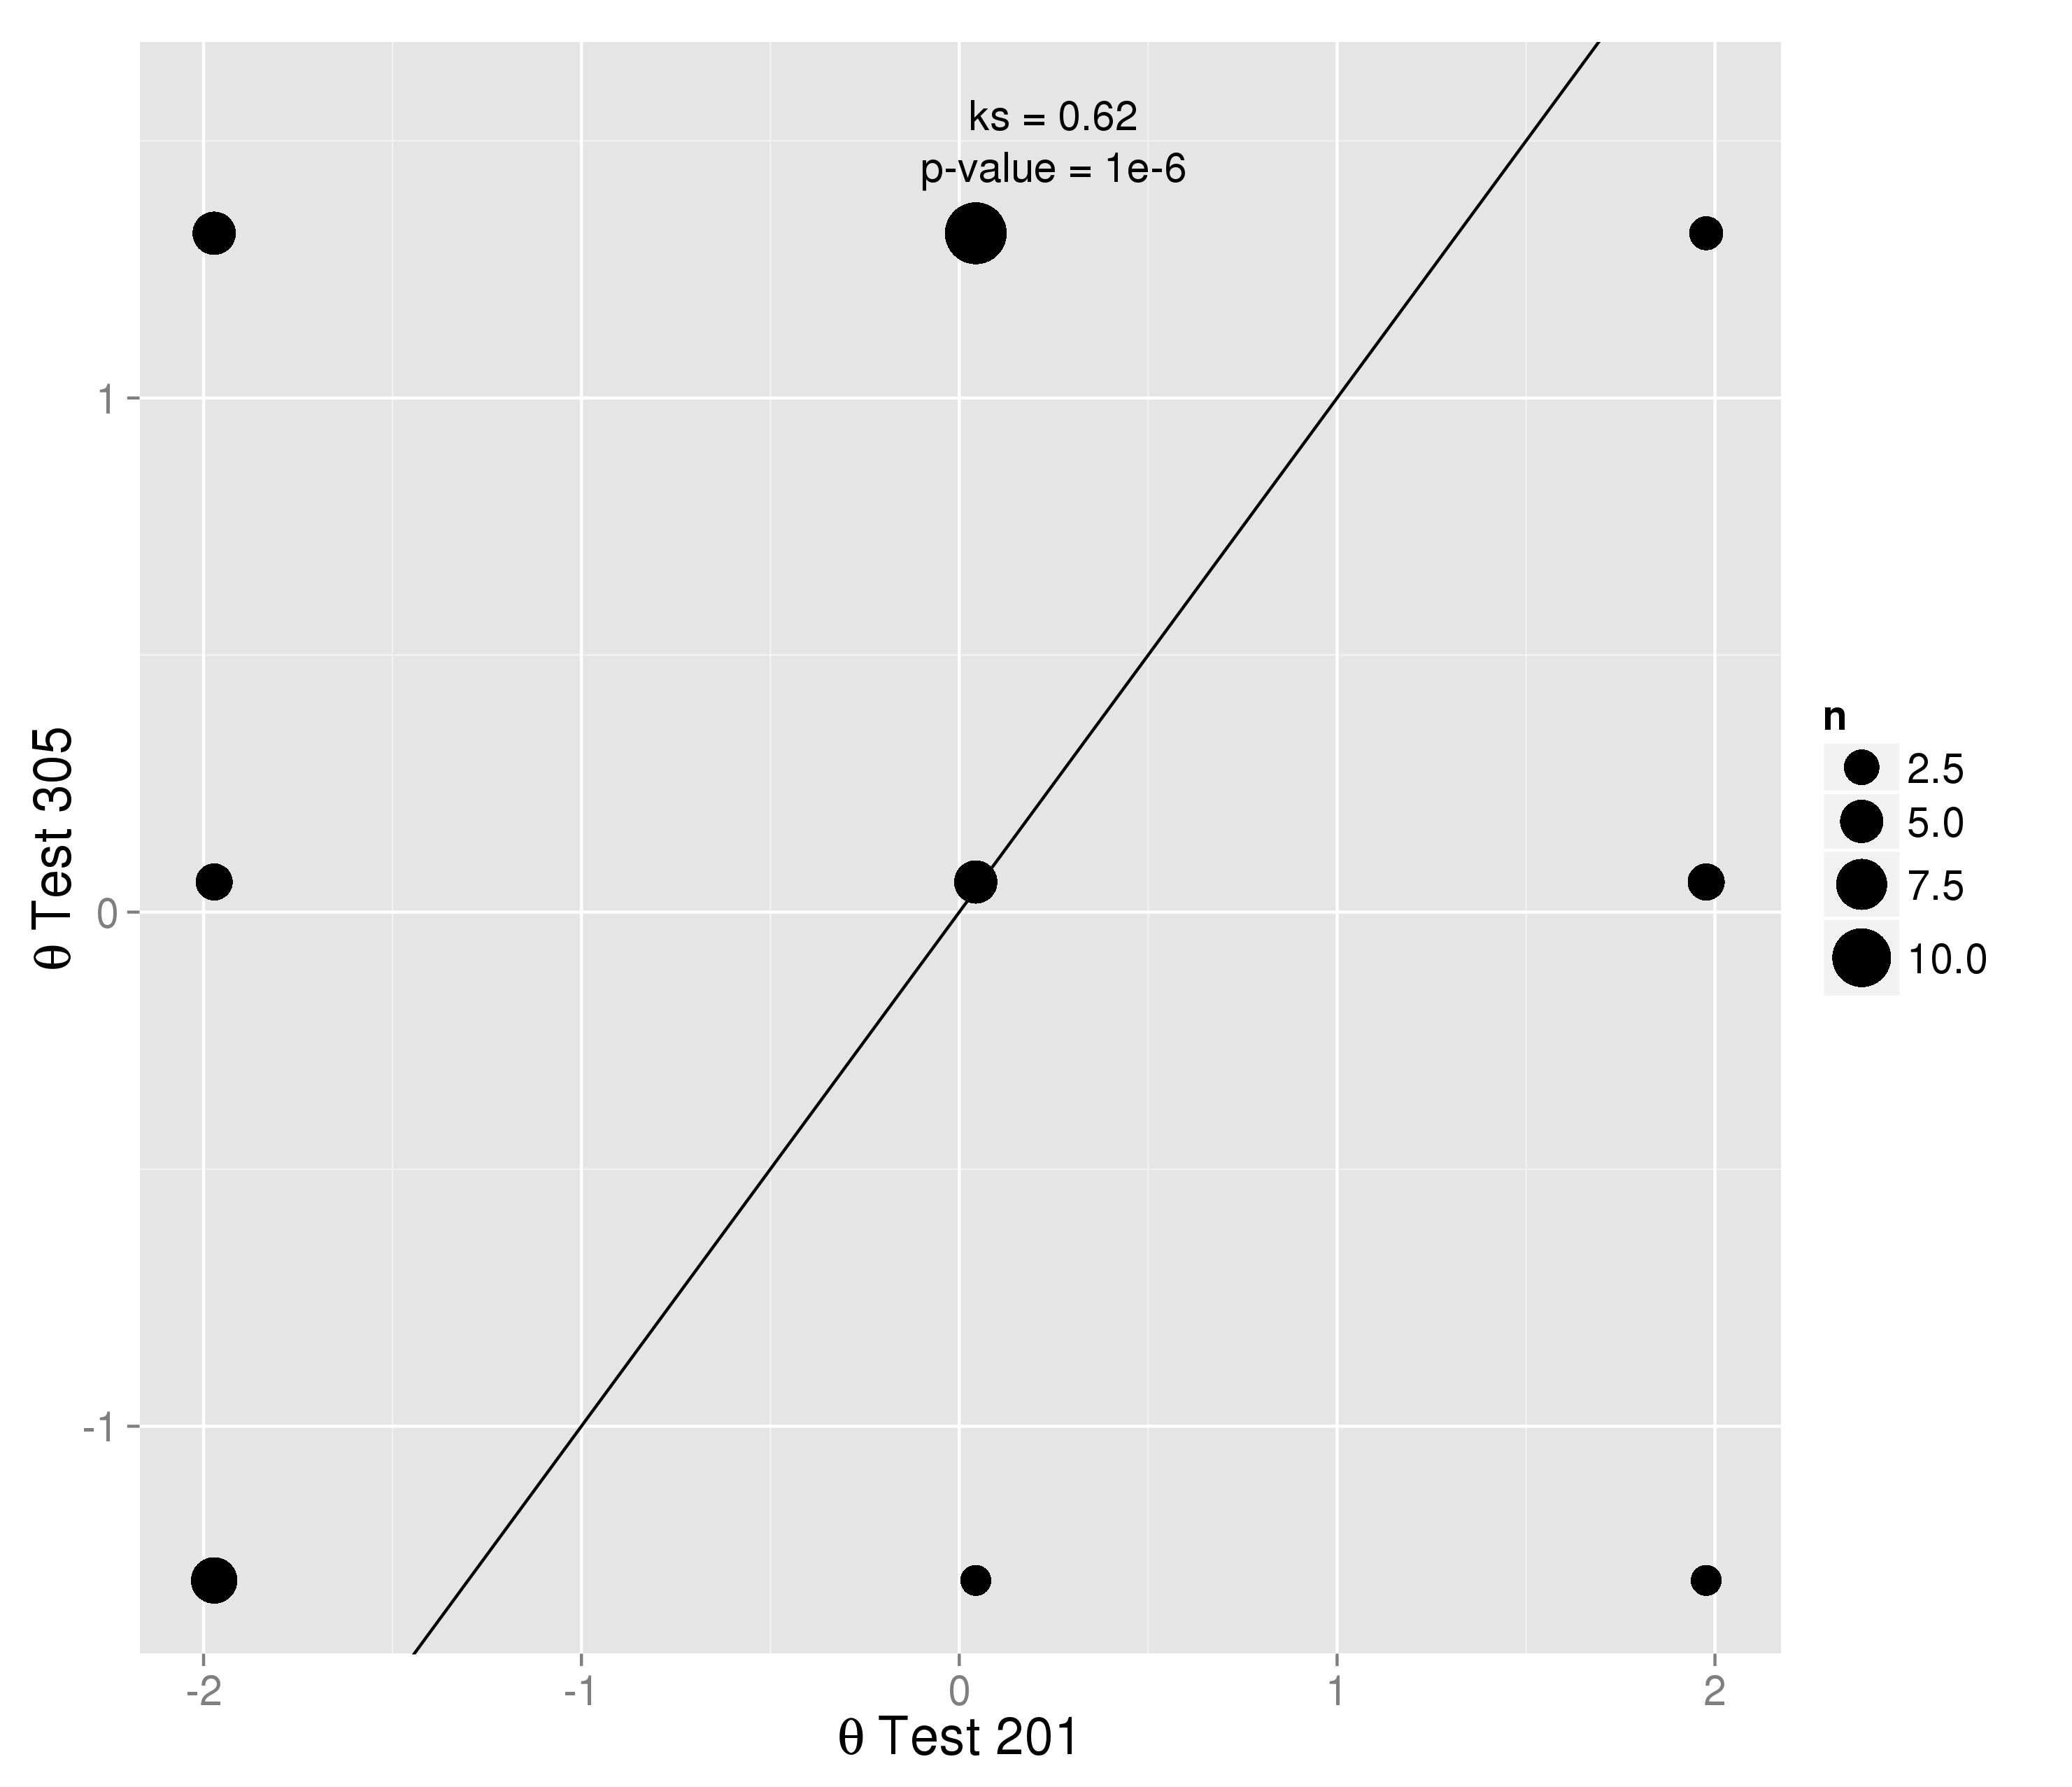
\includegraphics[width=1.0\linewidth]{graphics/GOF201305Pers.png}
   \caption{Vergleich der Personen-Parameter $\theta_i$ zwischen Test 201 und 305.}
   \label{fig:GOF201305P}
 \end{subfigure}

  \begin{subfigure}{0.5\textwidth}
    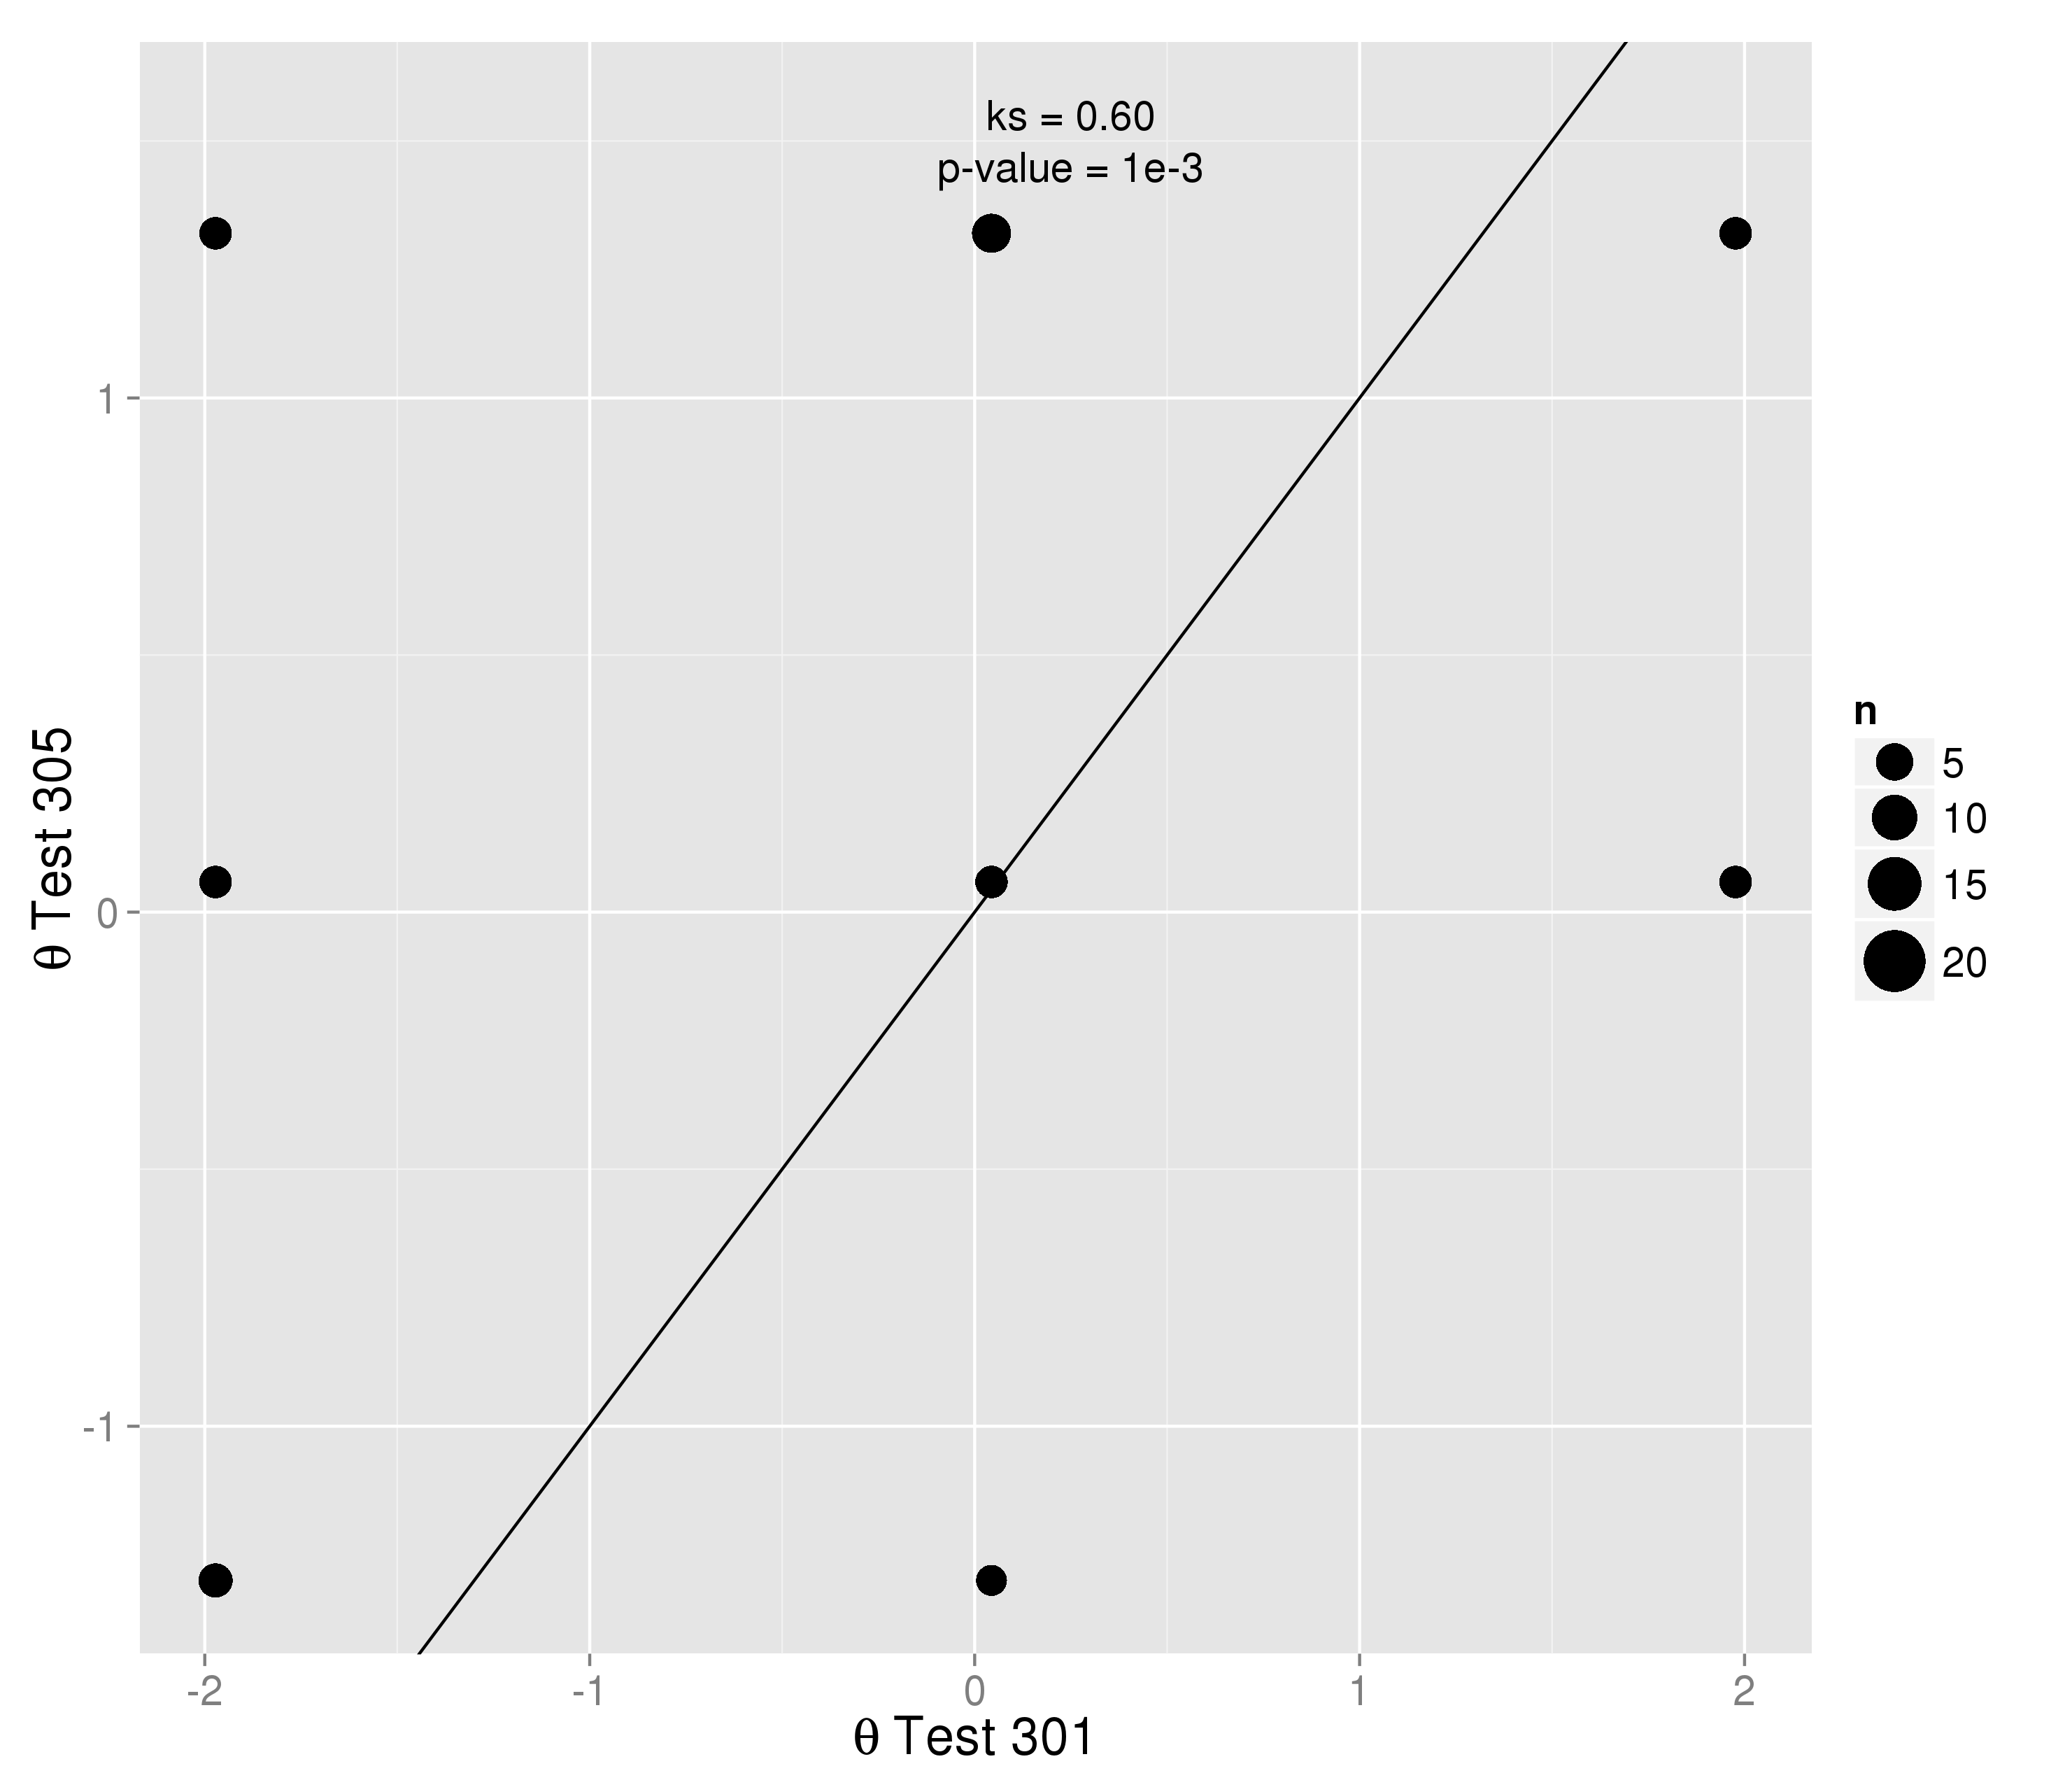
\includegraphics[width=1.0\linewidth]{graphics/GOF301305Pers.png}
    \caption{Vergleich der Personen-Parameter $\theta_i$ zwischen Test 301 und 305.}
    \label{fig:GOF301305P}
  \end{subfigure}
 
 \caption{Vergleich der Personenparameter für die drei Tests. Zusätzlich sind der P-Wert des Kolmogorow-Smirnow-Test und die Test-Statistik $ks$ angegeben.}
 \label{fig:GOFP}
 \end{figure}
 
\github{http://git.io/FVjL}
\clearpage 
\subsection{Zusammenhang Rasch Modell und Fragebogen}

Hierfür wurde wieder das erste Rasch Modell verwendet, bei dem die Qualitätsstandards 1 bis 3 als Items verwendet wurden und pro Person nur eine Personen-Fähigkeit geschätzt wurde.
Die so geschätzten Personen-Fähigkeiten wurden mit den Ergebnissen des Fragebogens korreliert. Die Resultate befinden sich in den Darstellungen  und die Testergebnisse nochmals zusammengefasst in Tabelle.

\begin{table}[htbp]
  \centering
\begin{tabular}{@{}lllllllllll@{}}
\toprule
   \multicolumn{2}{l}{Note Mathe} &&  \multicolumn{2}{l}{Note NatW.}&&  \multicolumn{2}{l}{SESSKO}&&  \multicolumn{2}{l}{Selbskonzept Schulversuche}\\ 
      \cmidrule{1-2}\cmidrule{4-5}\cmidrule{7-8}\cmidrule{10-11}
   p-Wert & $\rho$ && p-Wert & $\rho$  && p-Wert & $\rho$&& p-Wert & $\rho$\\ 
\midrule
   0.16 & 0.17 && 0.95 & 0.0 && 0.46 & 0.09 && 0.04 & 0.23    \\ 

\bottomrule
\end{tabular} 
  \caption{Spearmans $\rho$ und p-Werte für die Korrelation zwischen der Personen-Fähigkeit $\theta$ und verschiedenen Skalen.  }
  \label{tab:CorPersonRasch}
\end{table}

 \begin{figure}[htp]
 \centering
 \begin{subfigure}{0.49\textwidth}
   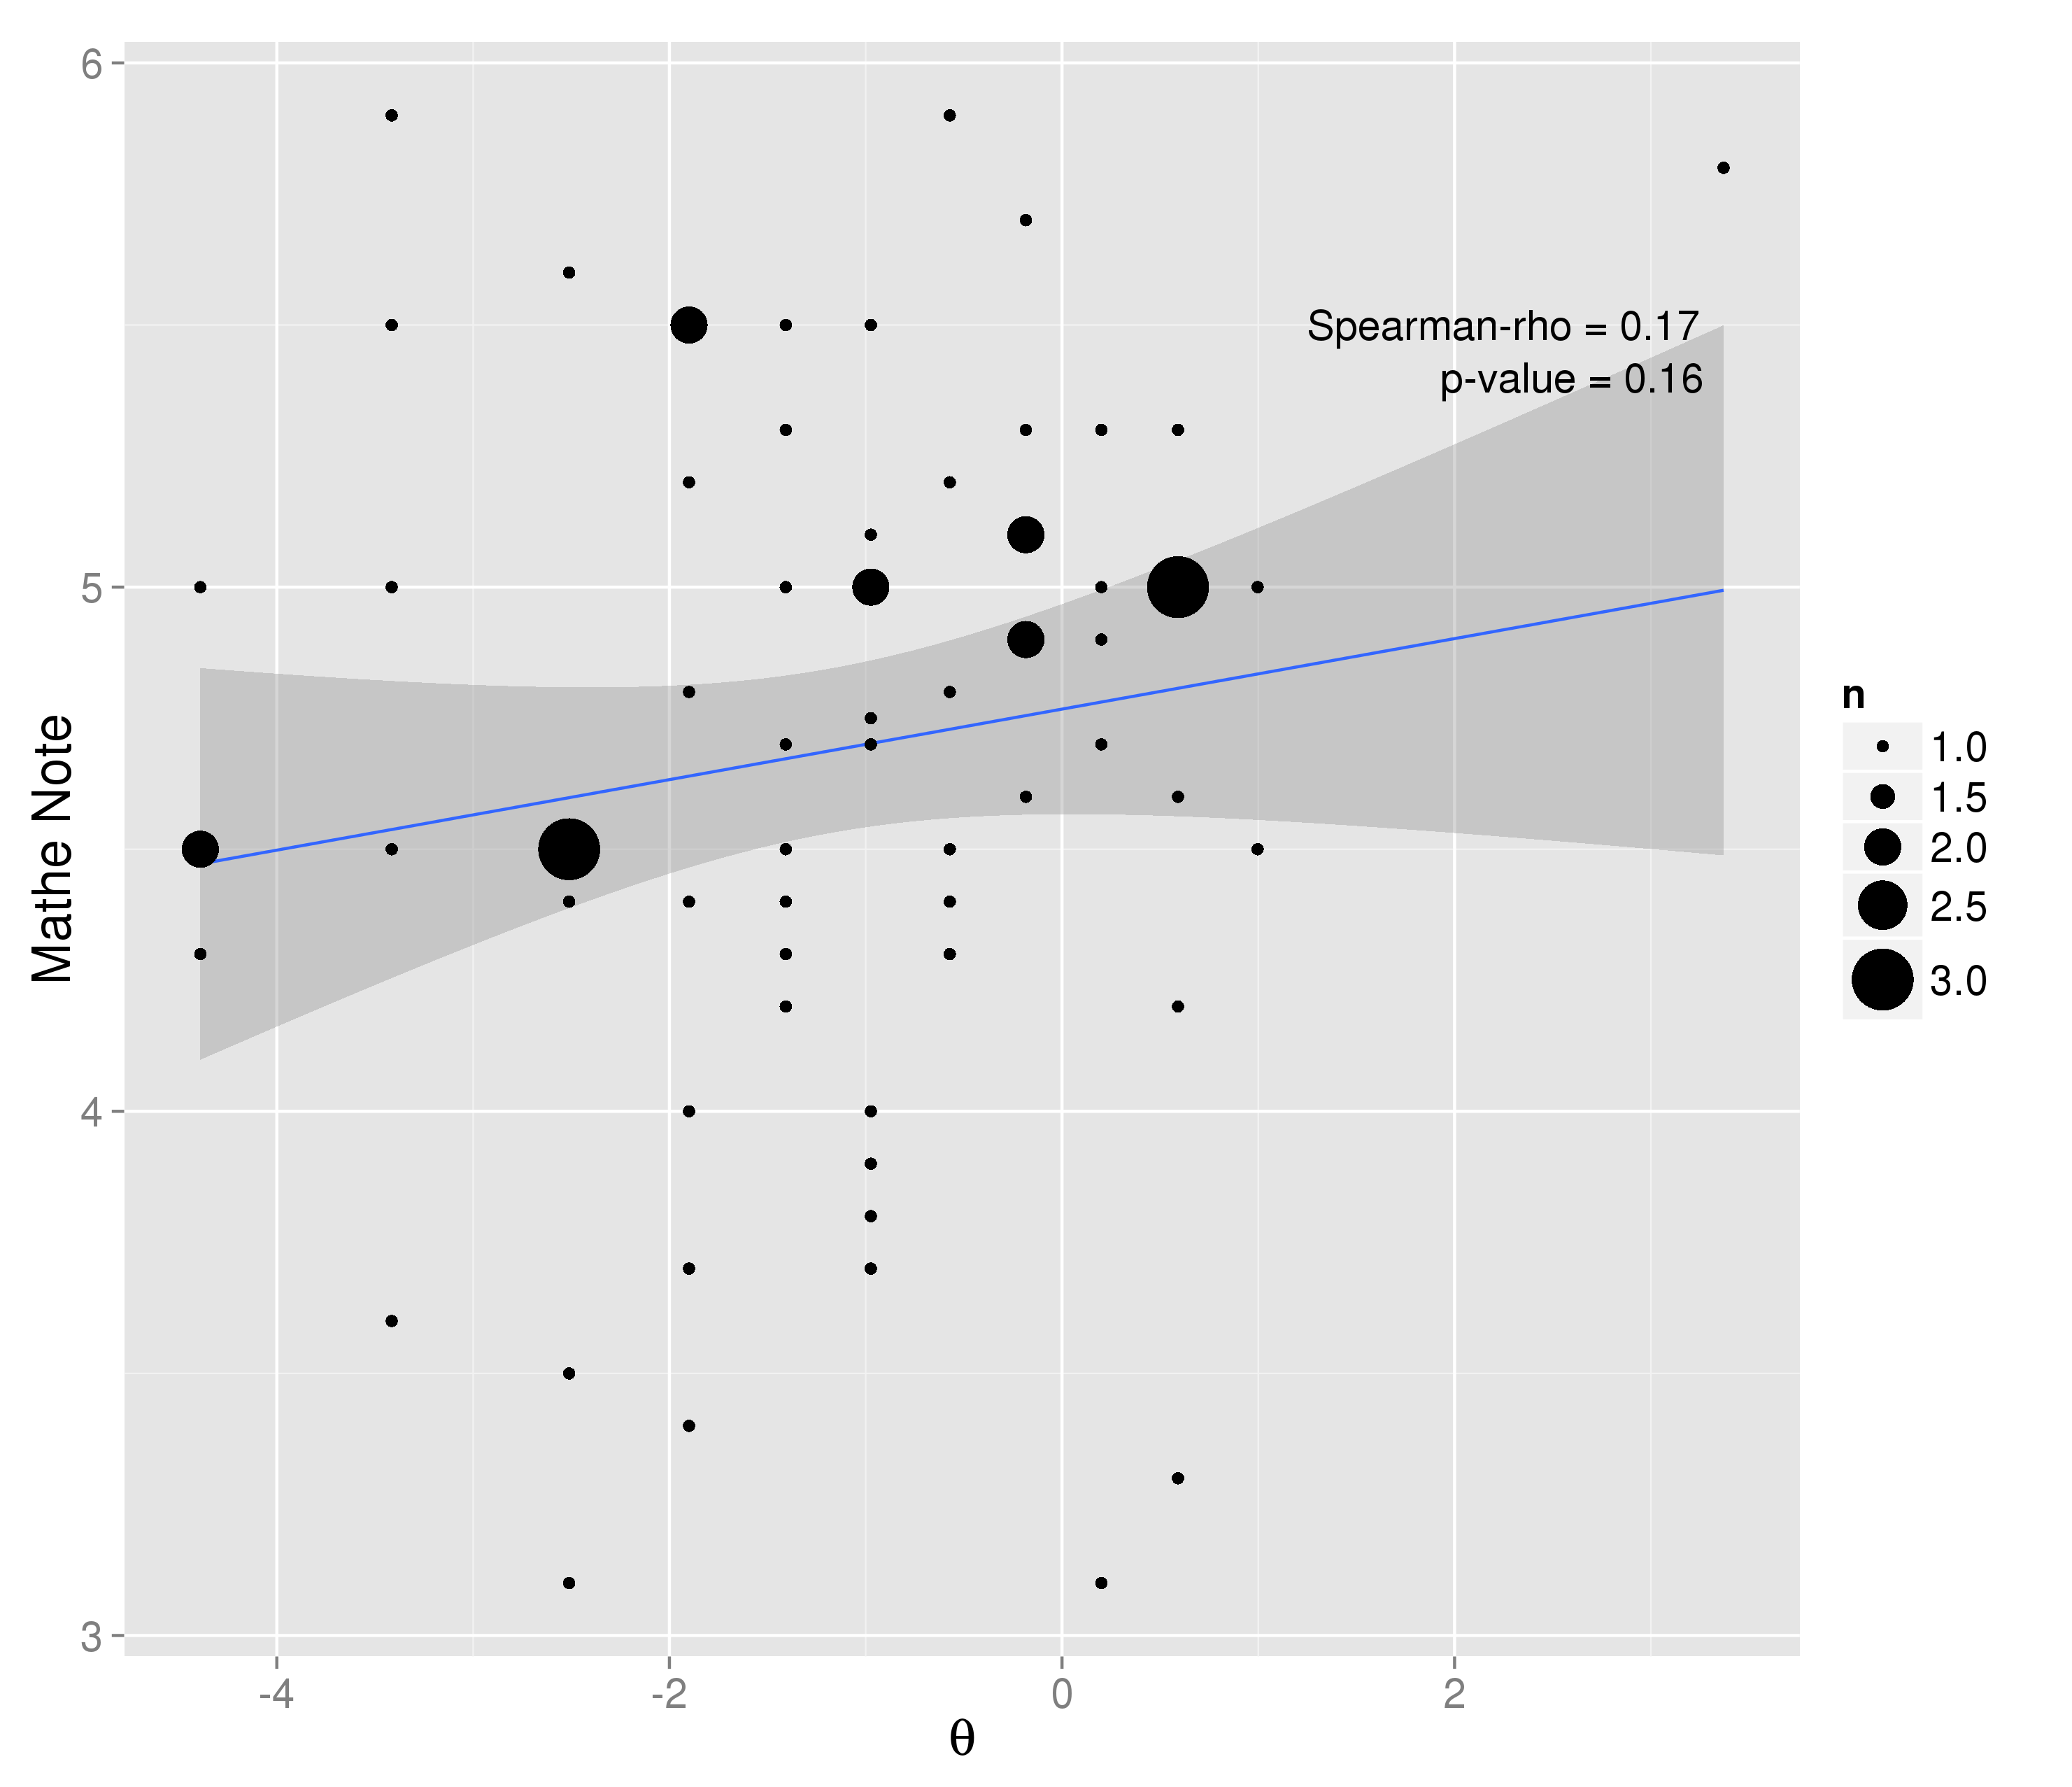
\includegraphics[width=1.0\linewidth]{graphics/corPersonenMathe.png}
   \caption{Korrelation der Personen-Fähigkeit $\theta$ mit der Note in Mathe.}
   \label{fig:corPersonenMathe}
 \end{subfigure}
 \begin{subfigure}{0.49\textwidth}
   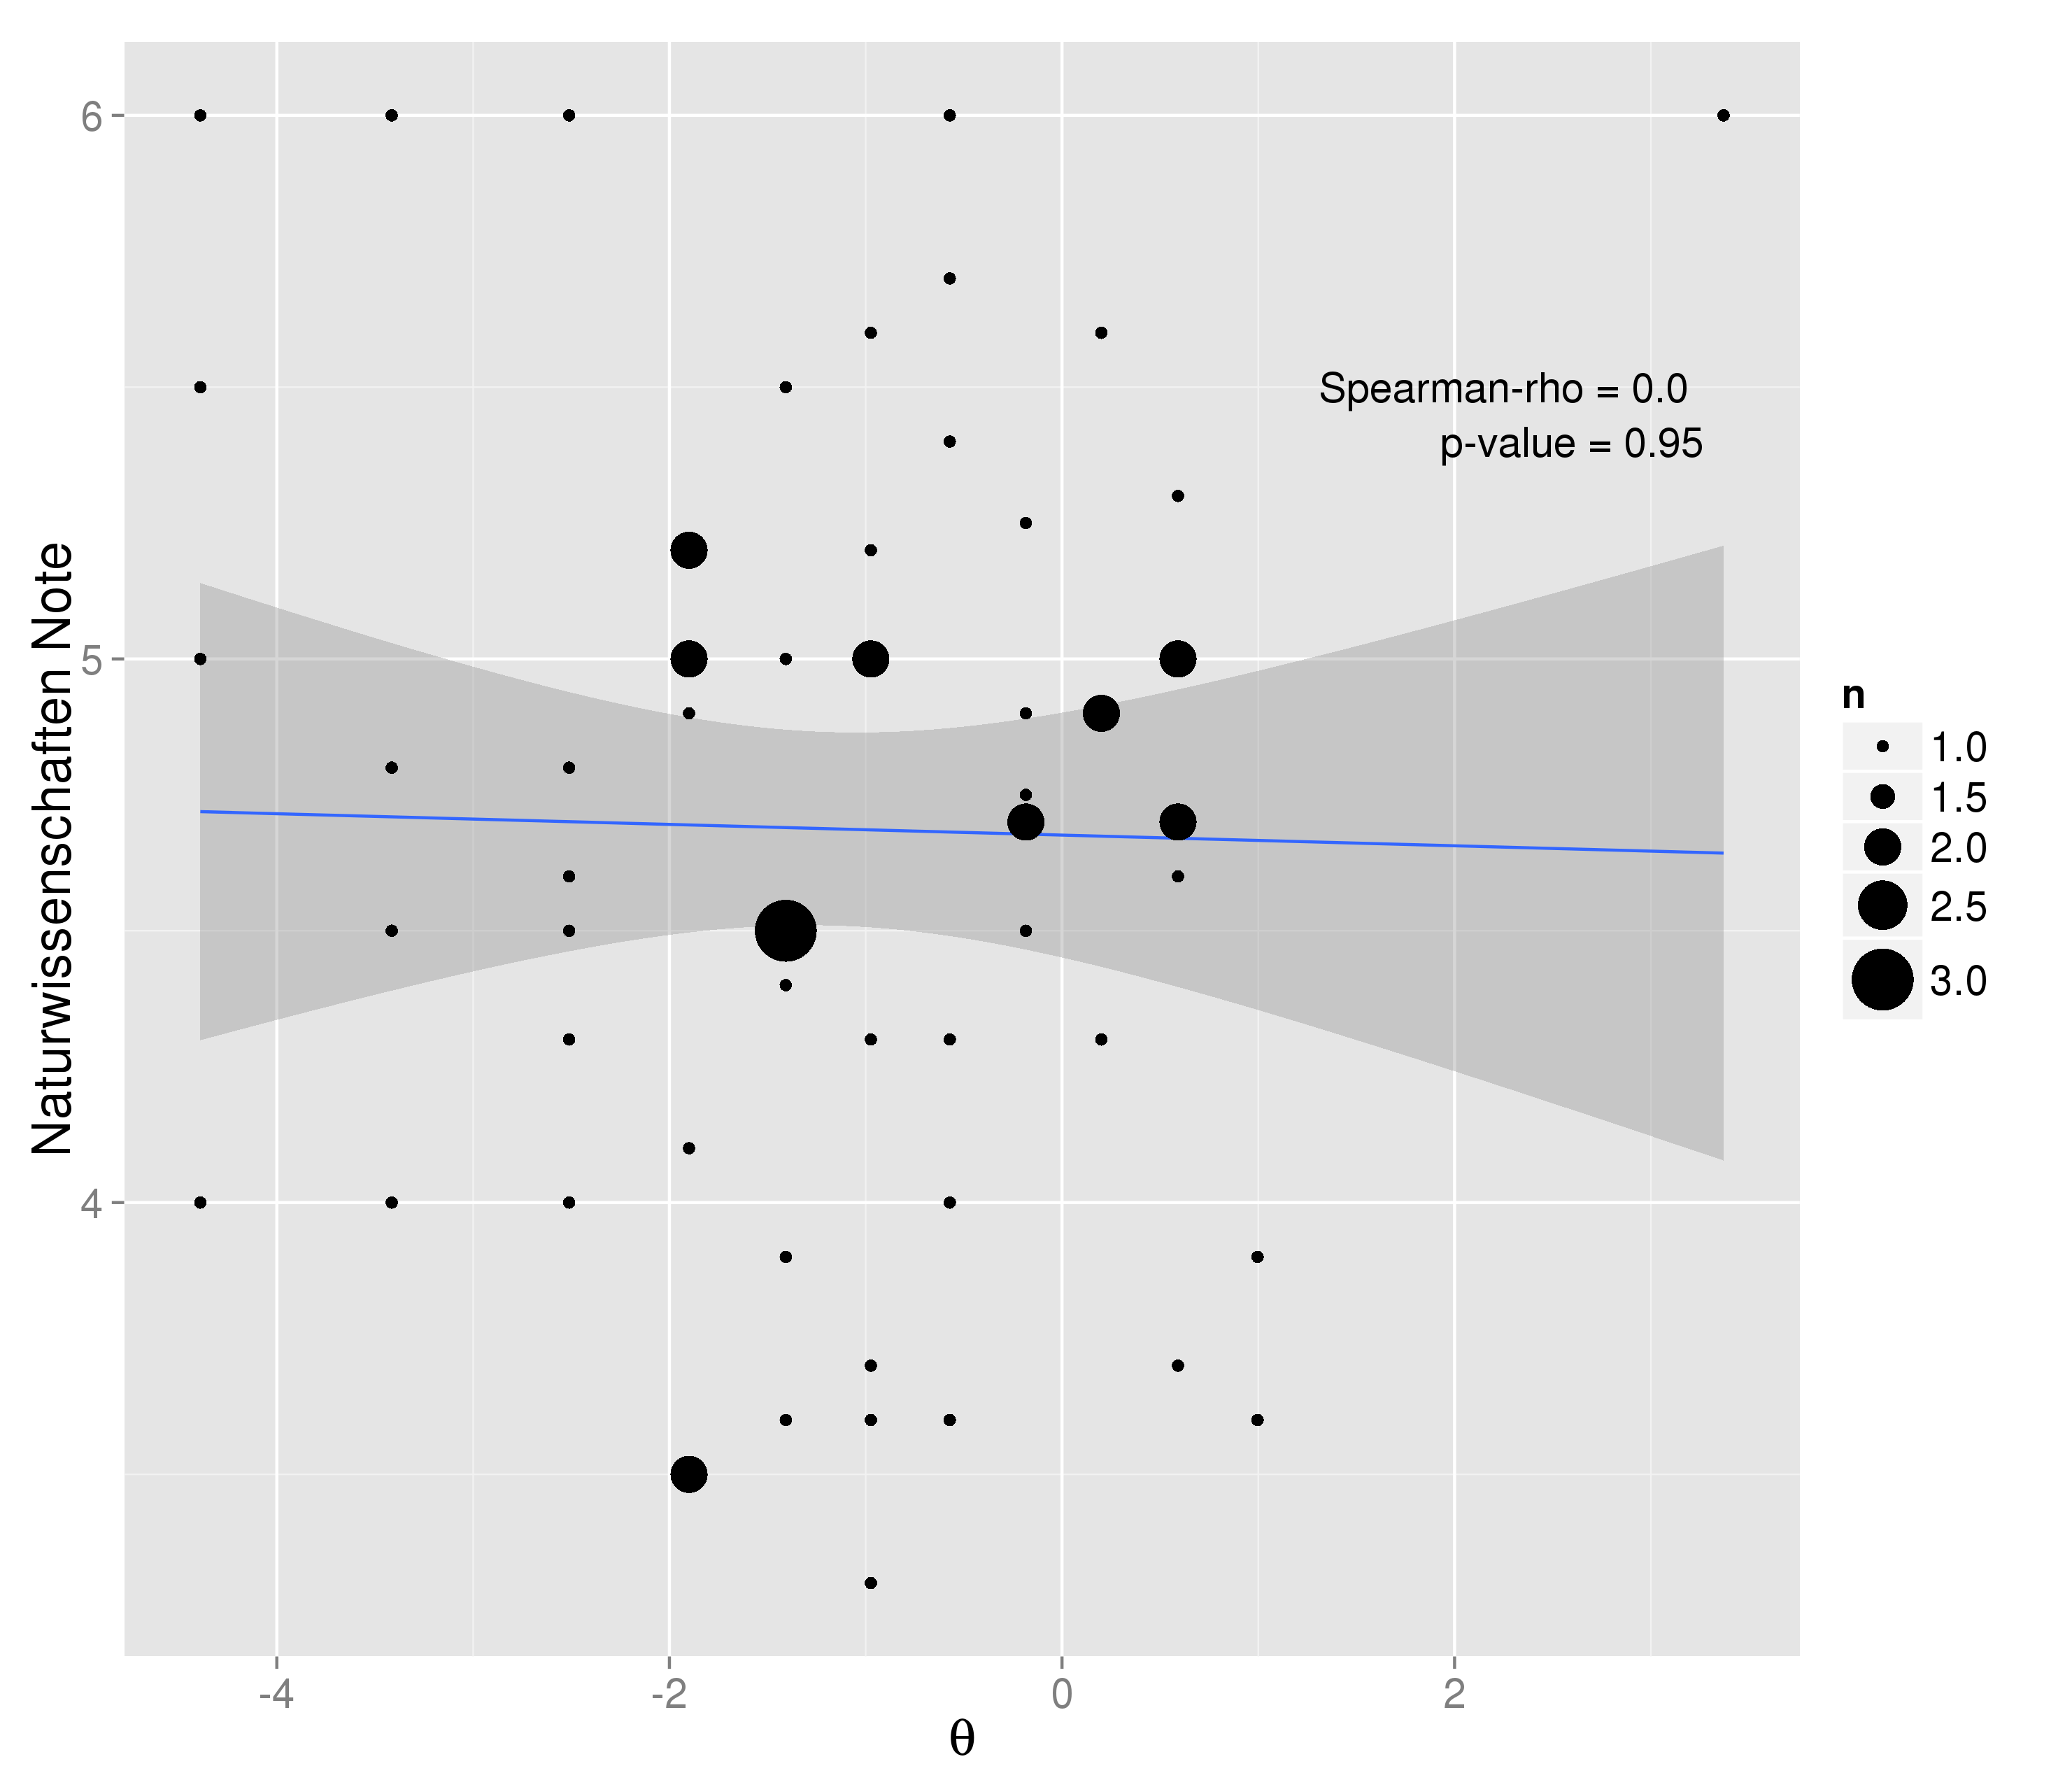
\includegraphics[width=1.0\linewidth]{graphics/corPersonenNatw.png}
   \caption{Korrelation der Personen-Fähigkeit $\theta$ mit der Note in den Naturwissenschaften.}
   \label{fig:corPersonenNatW}
 \end{subfigure}
  \end{figure}
  \begin{figure}[htbp]
  \ContinuedFloat % continue from previous page
  \centering
  \begin{subfigure}{0.49\textwidth}
   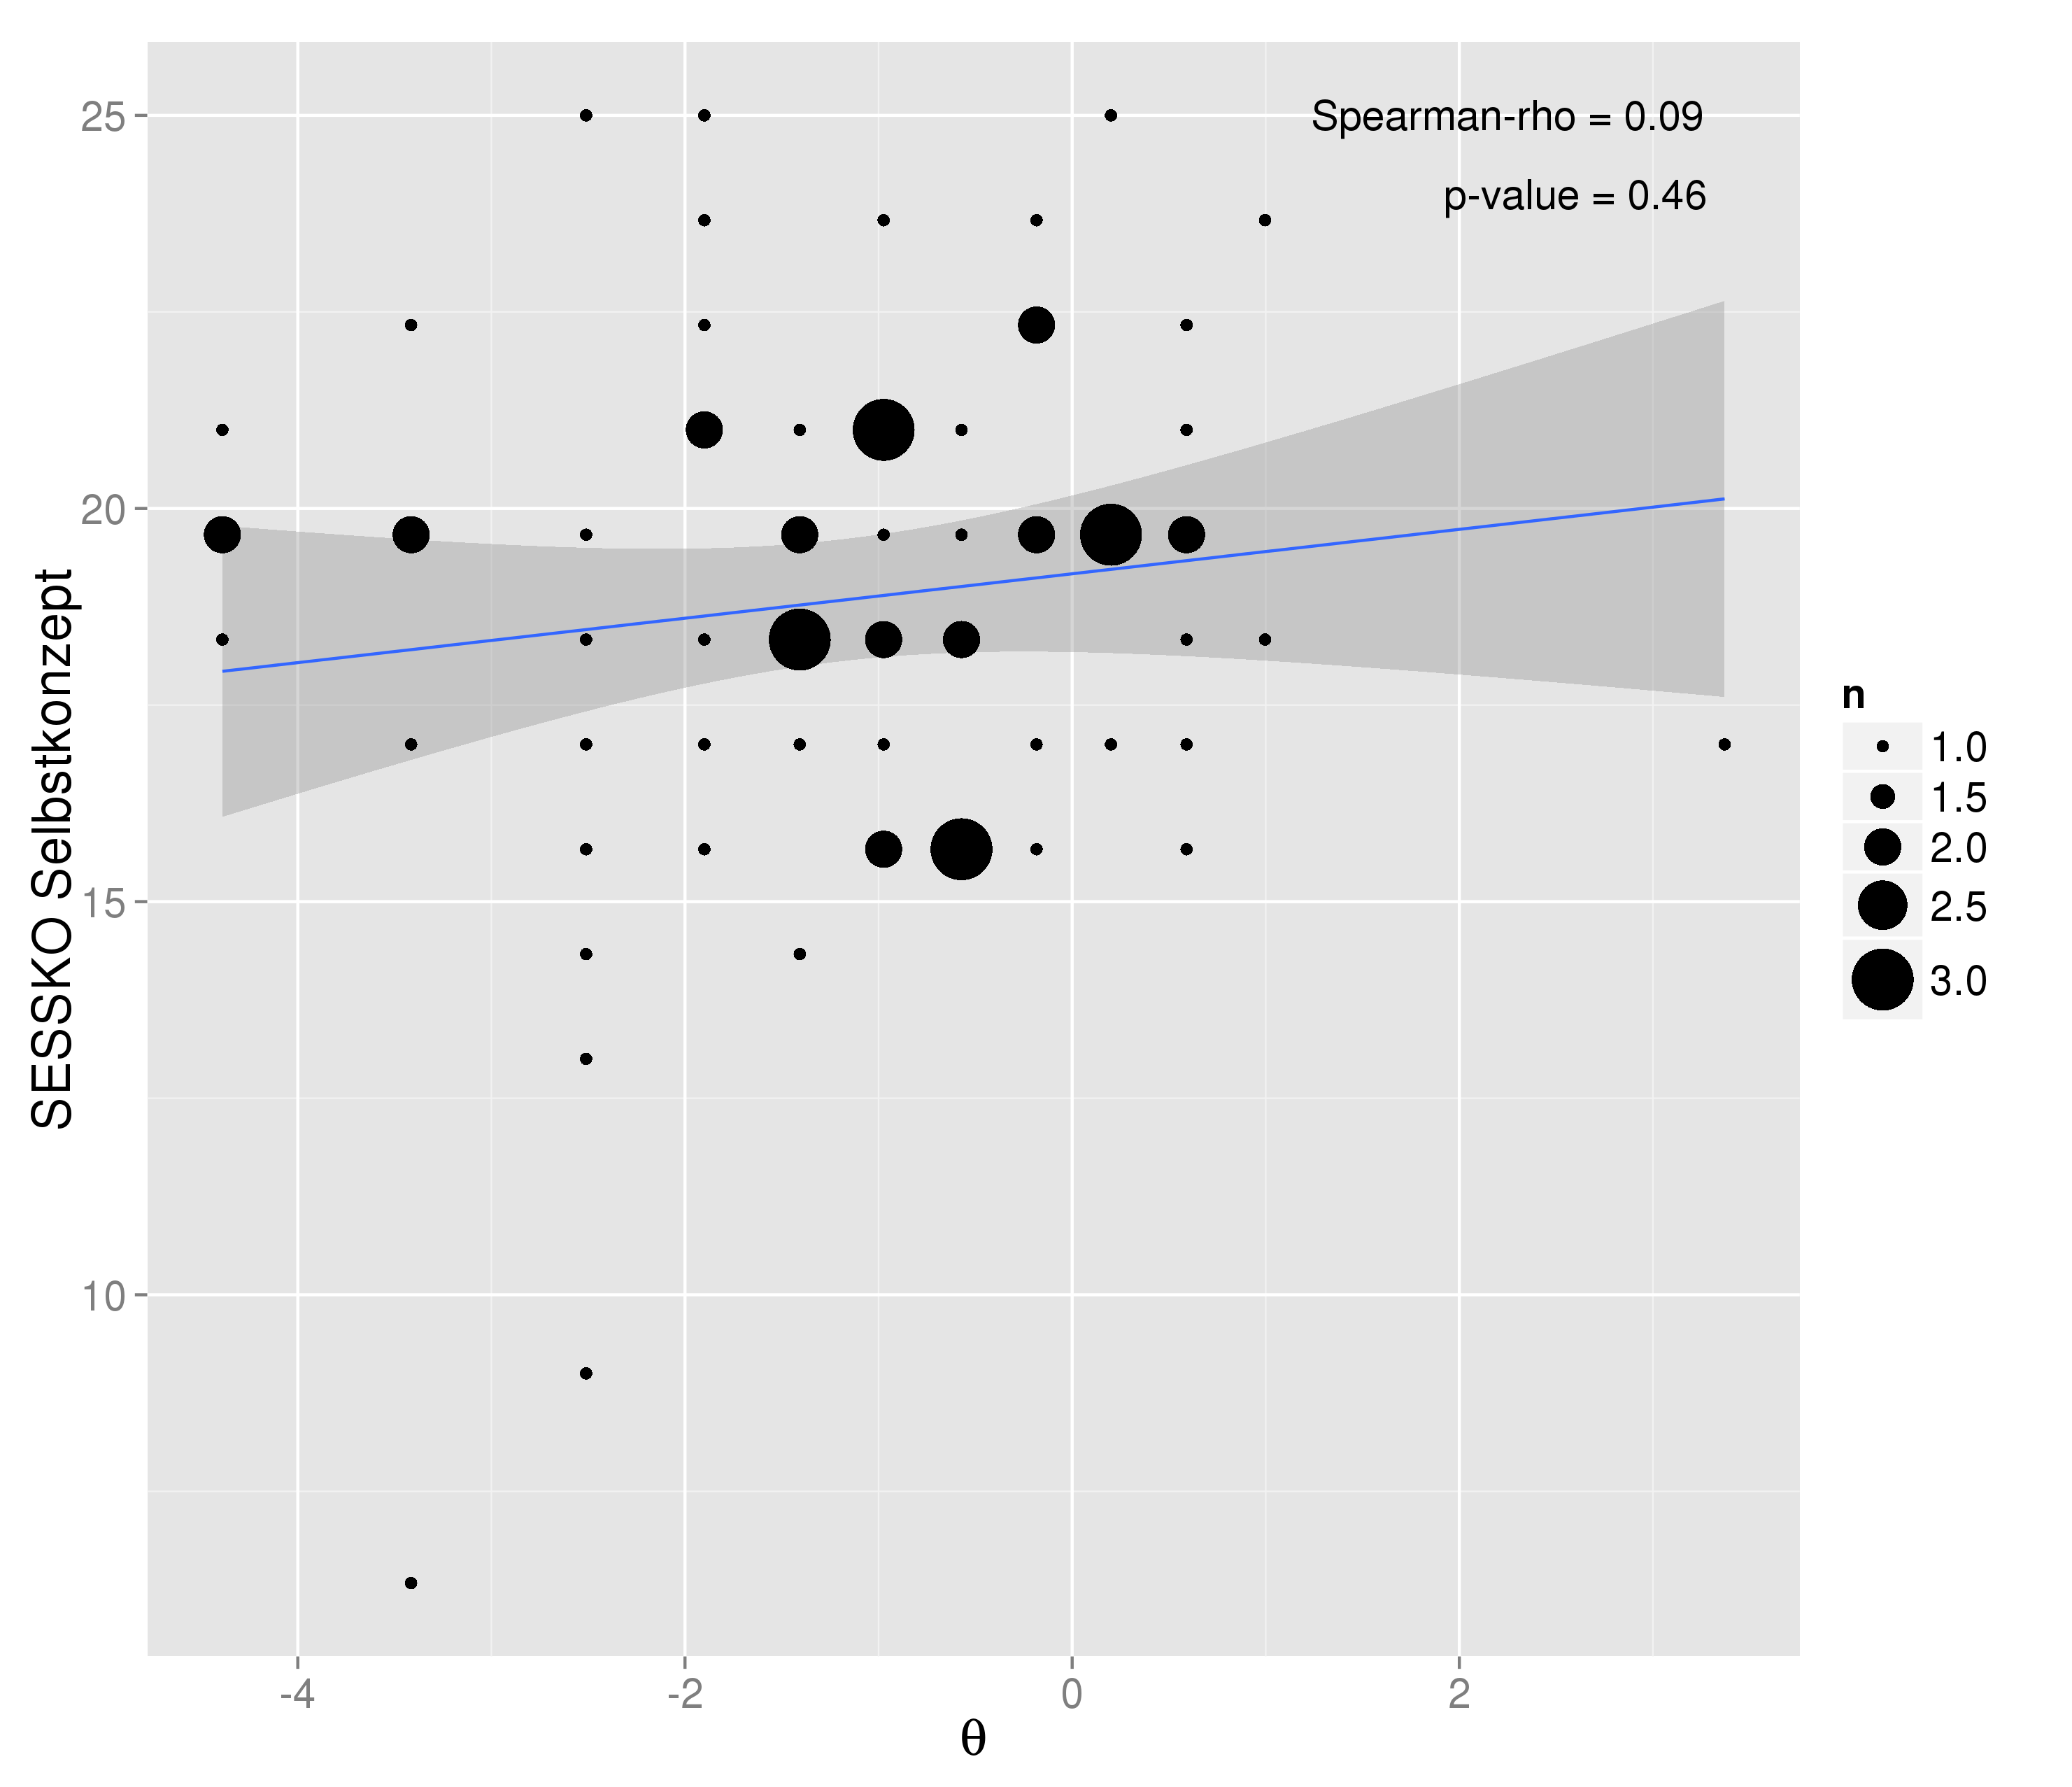
\includegraphics[width=1.0\linewidth]{graphics/corPersonenSESSKO.png}
   \caption{Korrelation der Personen-Fähigkeit $\theta$ mit dem absoluten Schulischem Selbstkonzept nach SESSKO \citep{Schone2002}.}
   \label{fig:corPersonenSESSKO}
  \end{subfigure}
  \begin{subfigure}{0.49\textwidth}
    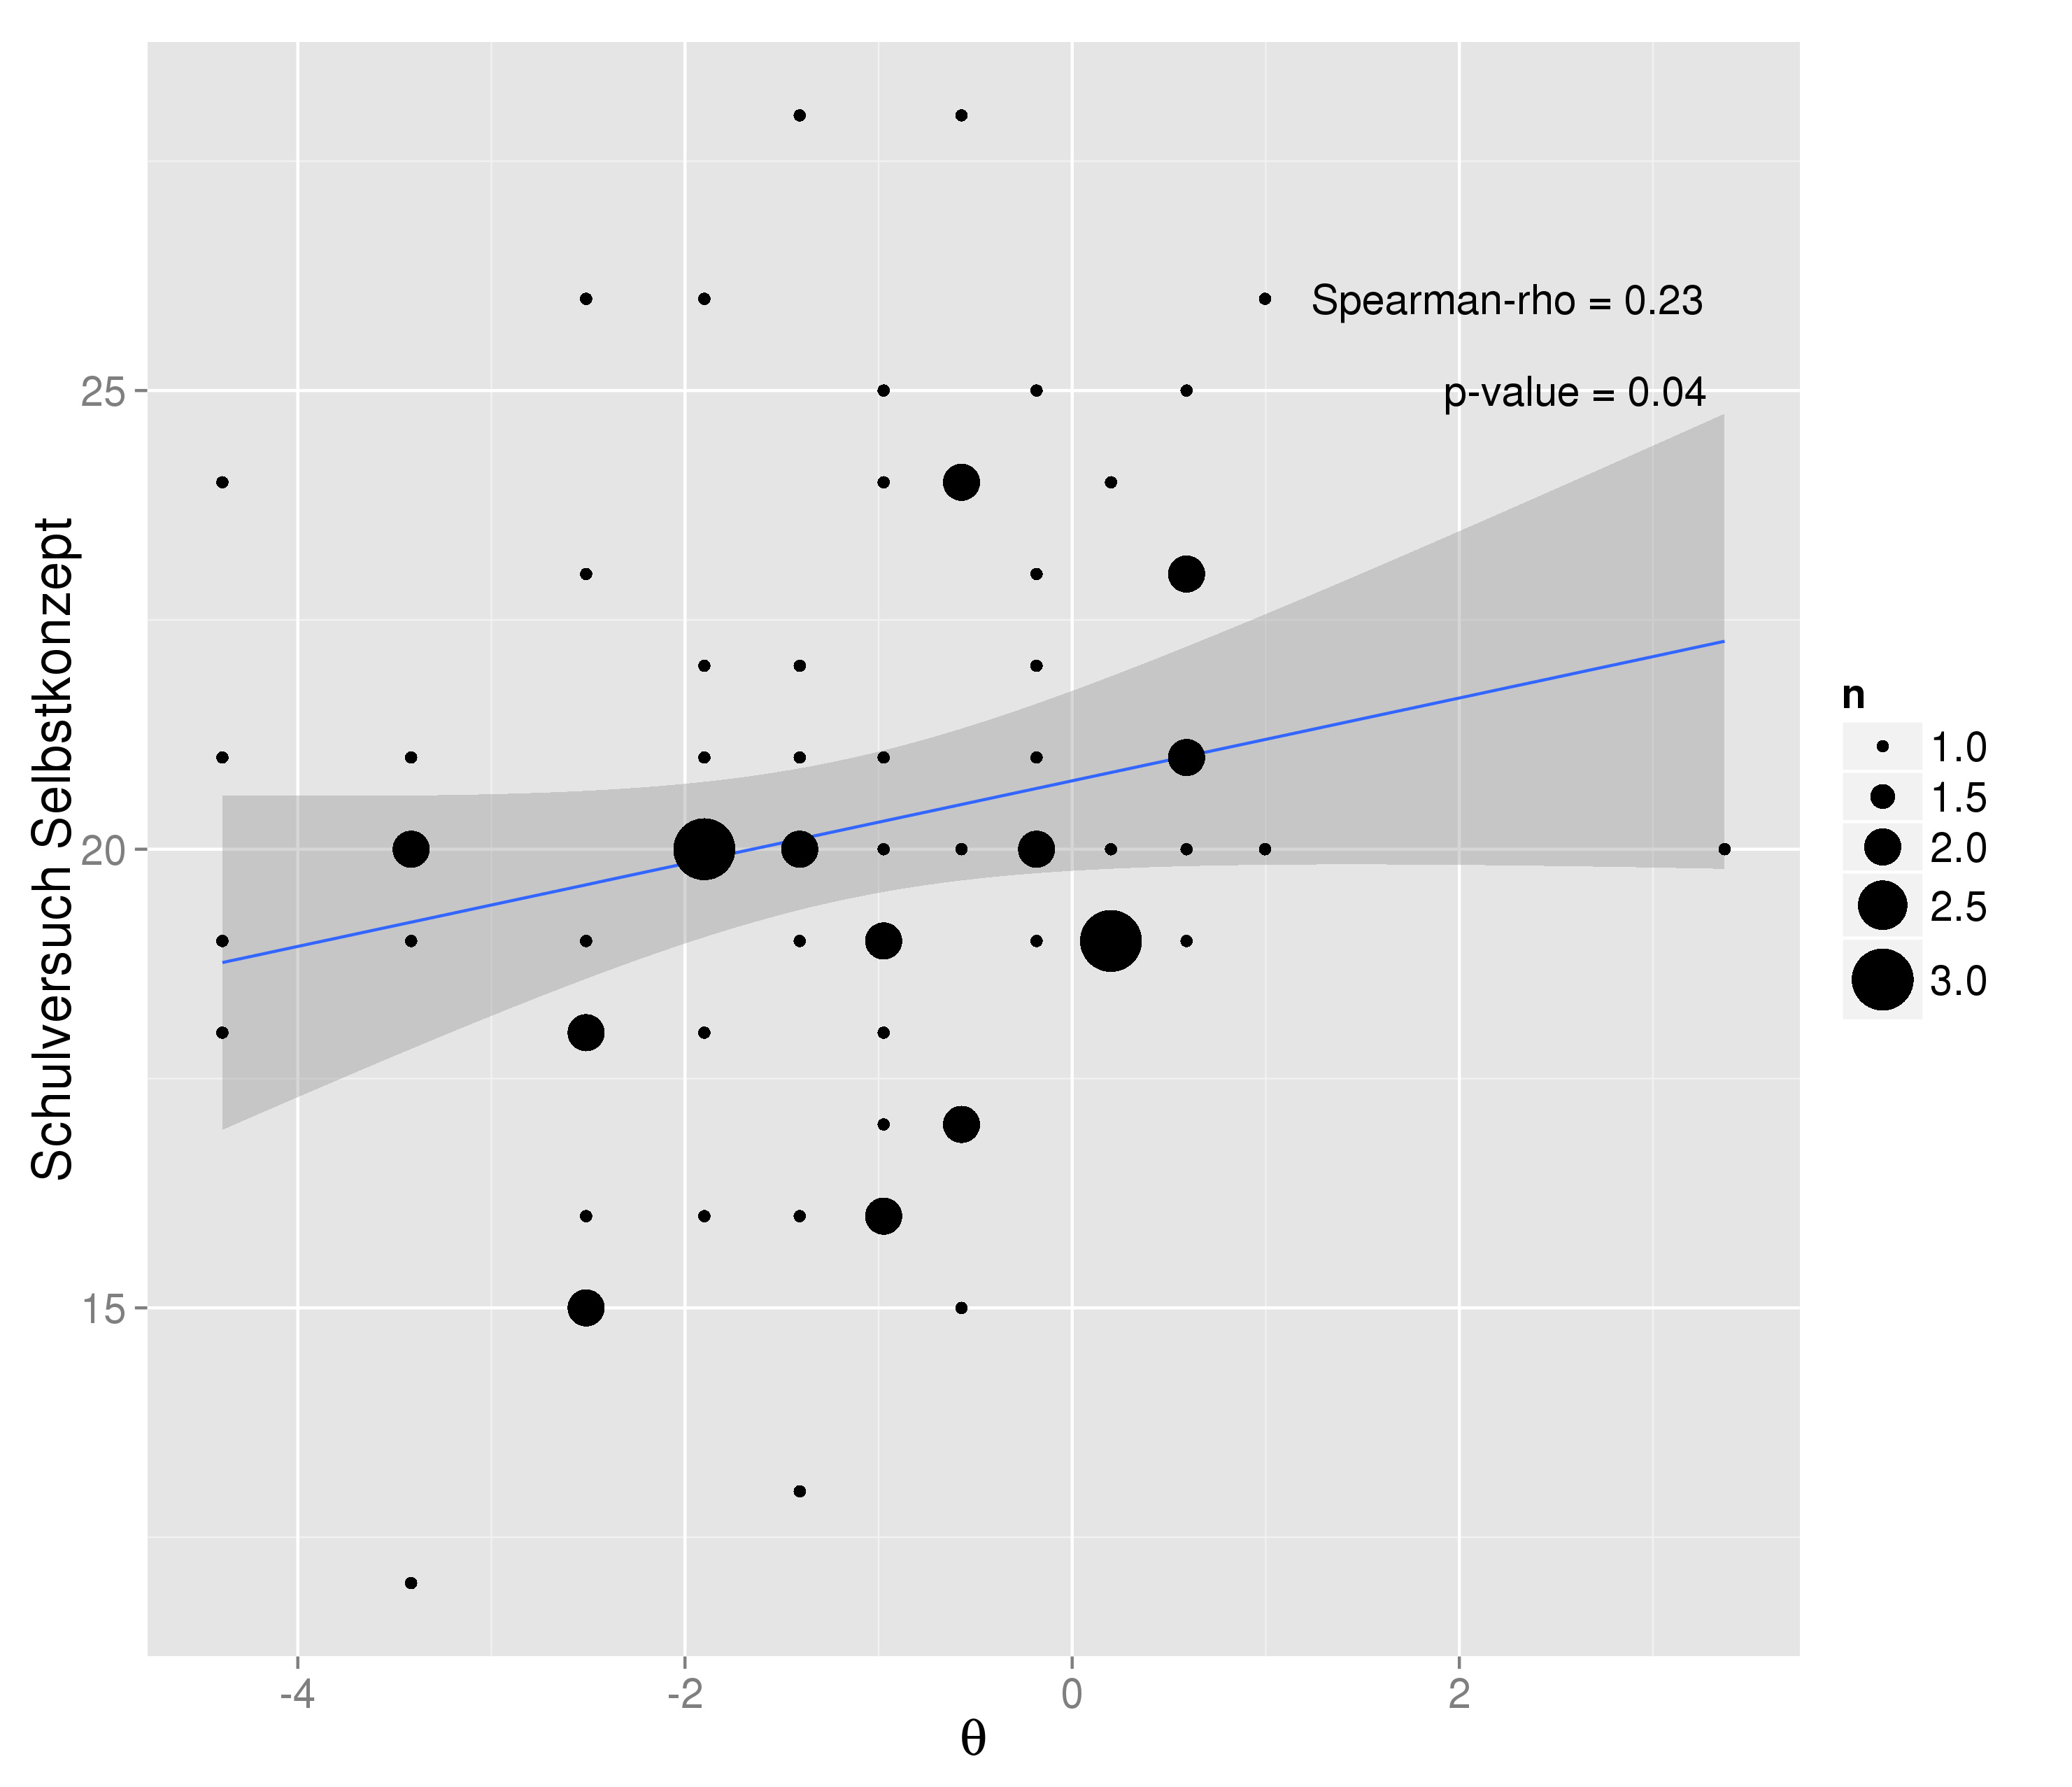
\includegraphics[width=1.0\linewidth]{graphics/corPersonenSelbskonzept.png}
    \caption{Korrelation der Personen-Fähigkeit $\theta$ mit dem Selbstkonzept bei Schulversuchen.}
    \label{fig:corPersonenSelbskonzept}
  \end{subfigure}
 \caption{Korrelation zwischen der Personen-Fähigkeit $\theta$ und verschiedenen per Fragebogen erhobenen Daten. Der Durchmesser der Punkte ist ein Mass für die Anzahl an Datenpunkten, welche an dieser Position liegen. Die blaue Gerade ist die lineare Regression der zugrunde liegenden Daten, der dunkel graue Bereich stellt das Vertrauensintervall (95\%) der linearen Regression dar. Zusätzlich sind noch Spearmans $rho$ und der p-Wert des Signifikanztests angegeben.}
 \label{fig:corPersonen}
 \end{figure}
 \github{http://git.io/FwCx}
 
 \clearpage
 \section{Videoanalyse}
 
 Insgesamt waren vier Stunden Videomaterial angefallen. Es wurde wie bereits erwähnt nur in einer Halbklasse eine Videoaufnahme durchgeführt. Aufgrund der Position der Videokamera konnten nur die Aktionen von je zwei Schülern und Schülerinnen analysiert werden. So konnten von 8 Schülerinnen und Schülern die Aktionen per Video analysiert werden.
 
 \subsection{Qualitätsstandards}
 
 Es wurden die existierende Qualitätsstandards auf Überprüfbarkeit per Video analysiert. Es wurden die Qualitätsstandards 1 und 4 als analysierbar identifiziert. Für diese beiden Standards wurde jeweils eine Kodierung definiert.
 
 \subsubsection{Korrekt und präzise messen}
 
 Es wurde eine Kodierung, welche an \citet{Schreiber2012} angelehnt war verwendet. Bei der Kodierung des Merkmales korrekt und präzise messen wurde von einer Gütestufe von 3 ausgegangen. Wenn ein Schüler oder Schülerin nicht korrekt abgemessen hat (z.B. schräg abgelesen), wurde Gütestufe 2 kodiert. Wenn die Schülerin oder der Schüler bei den einzelnen Messungen unterschiedlich gemessen hat, wurde die Gütestufe 1 vergeben.
 
 \subsubsection{Messung wiederholen}
 
 Bei diesem Merkmal wurde von einer Gütestufe von 1 ausgegangen. Wenn der Schüler oder die Schülerin die Messung wiederholt hat, wurde die Gütestufe 2 erreicht. Als Messwiederholung wurde eine Messung in einem neuen Experiment definiert. Es reichte also nicht, mehrmals die den Messwert abzulesen um diese Gütestufe zu erreichen, sondern es musste das Experiment erneut durchgeführt werden. Gütestufe 3 wurde erreicht, wenn das Experiment identisch durchgeführt wurde.
 
 Die Resultate der Kodierungen befinden sich in Tabelle \ref{tab:VideoMerkmale}.
 
 
 
 \begin{table}[htbp]
   \centering
 \begin{tabular}{@{}lllllllll@{}}
 \toprule
    &&\multicolumn{3}{l}{Messung korrekt} &&  \multicolumn{3}{l}{Messwiederholung.}\\ 
       \cmidrule{3-5}\cmidrule{7-9}
    Test && 1 & 2 & 3 && 1 & 2 & 3 \\ 
 \midrule
    201 && 0.25 & 0.63 & 0.13 && 0.63 & 0.38 & 0.00   \\ 
    301 && 0.13 & 0.75 & 0.13 && 0.63 & 0.38 & 0.00   \\ 
    305 && 0.25 & 0.63 & 0.13 && 0.38 & 0.38 & 0.25\\ 
 
 \bottomrule
 \end{tabular} 
   \caption{Die erreichten Gütestufen für die Merkmale Messung wiederholen und korrekt und präzise messen. Die Anzahl kodierter Personen beträgt 8.  }
   \label{tab:VideoMerkmale}
 \end{table}
 

 
 \subsection{Korrelation zwischen Video Merkmalen und Qualitätsstufen}
 
 Da die Videokodierung Merkmale basierend auf den Qualitätsstandards entwickelt hat, wurde untersucht ob zwischen den Merkmalen und den Qualitätsstandards eine Korrelation existiert. Diese Resultate befinden sich in Darstellung \ref{fig:corVideoQ} und in Tabelle \ref{tab:CorVideoQ}. In keinem der Korrelationstests wird die Signifikanz-schwelle überschritten, daher gibt es keine signifikante Korrelation zwischen den Qualitätsstandards und den Merkmalen der Videokodierung.
 
 \begin{figure}[htp]
  \centering
  \begin{subfigure}{0.32\textwidth}
    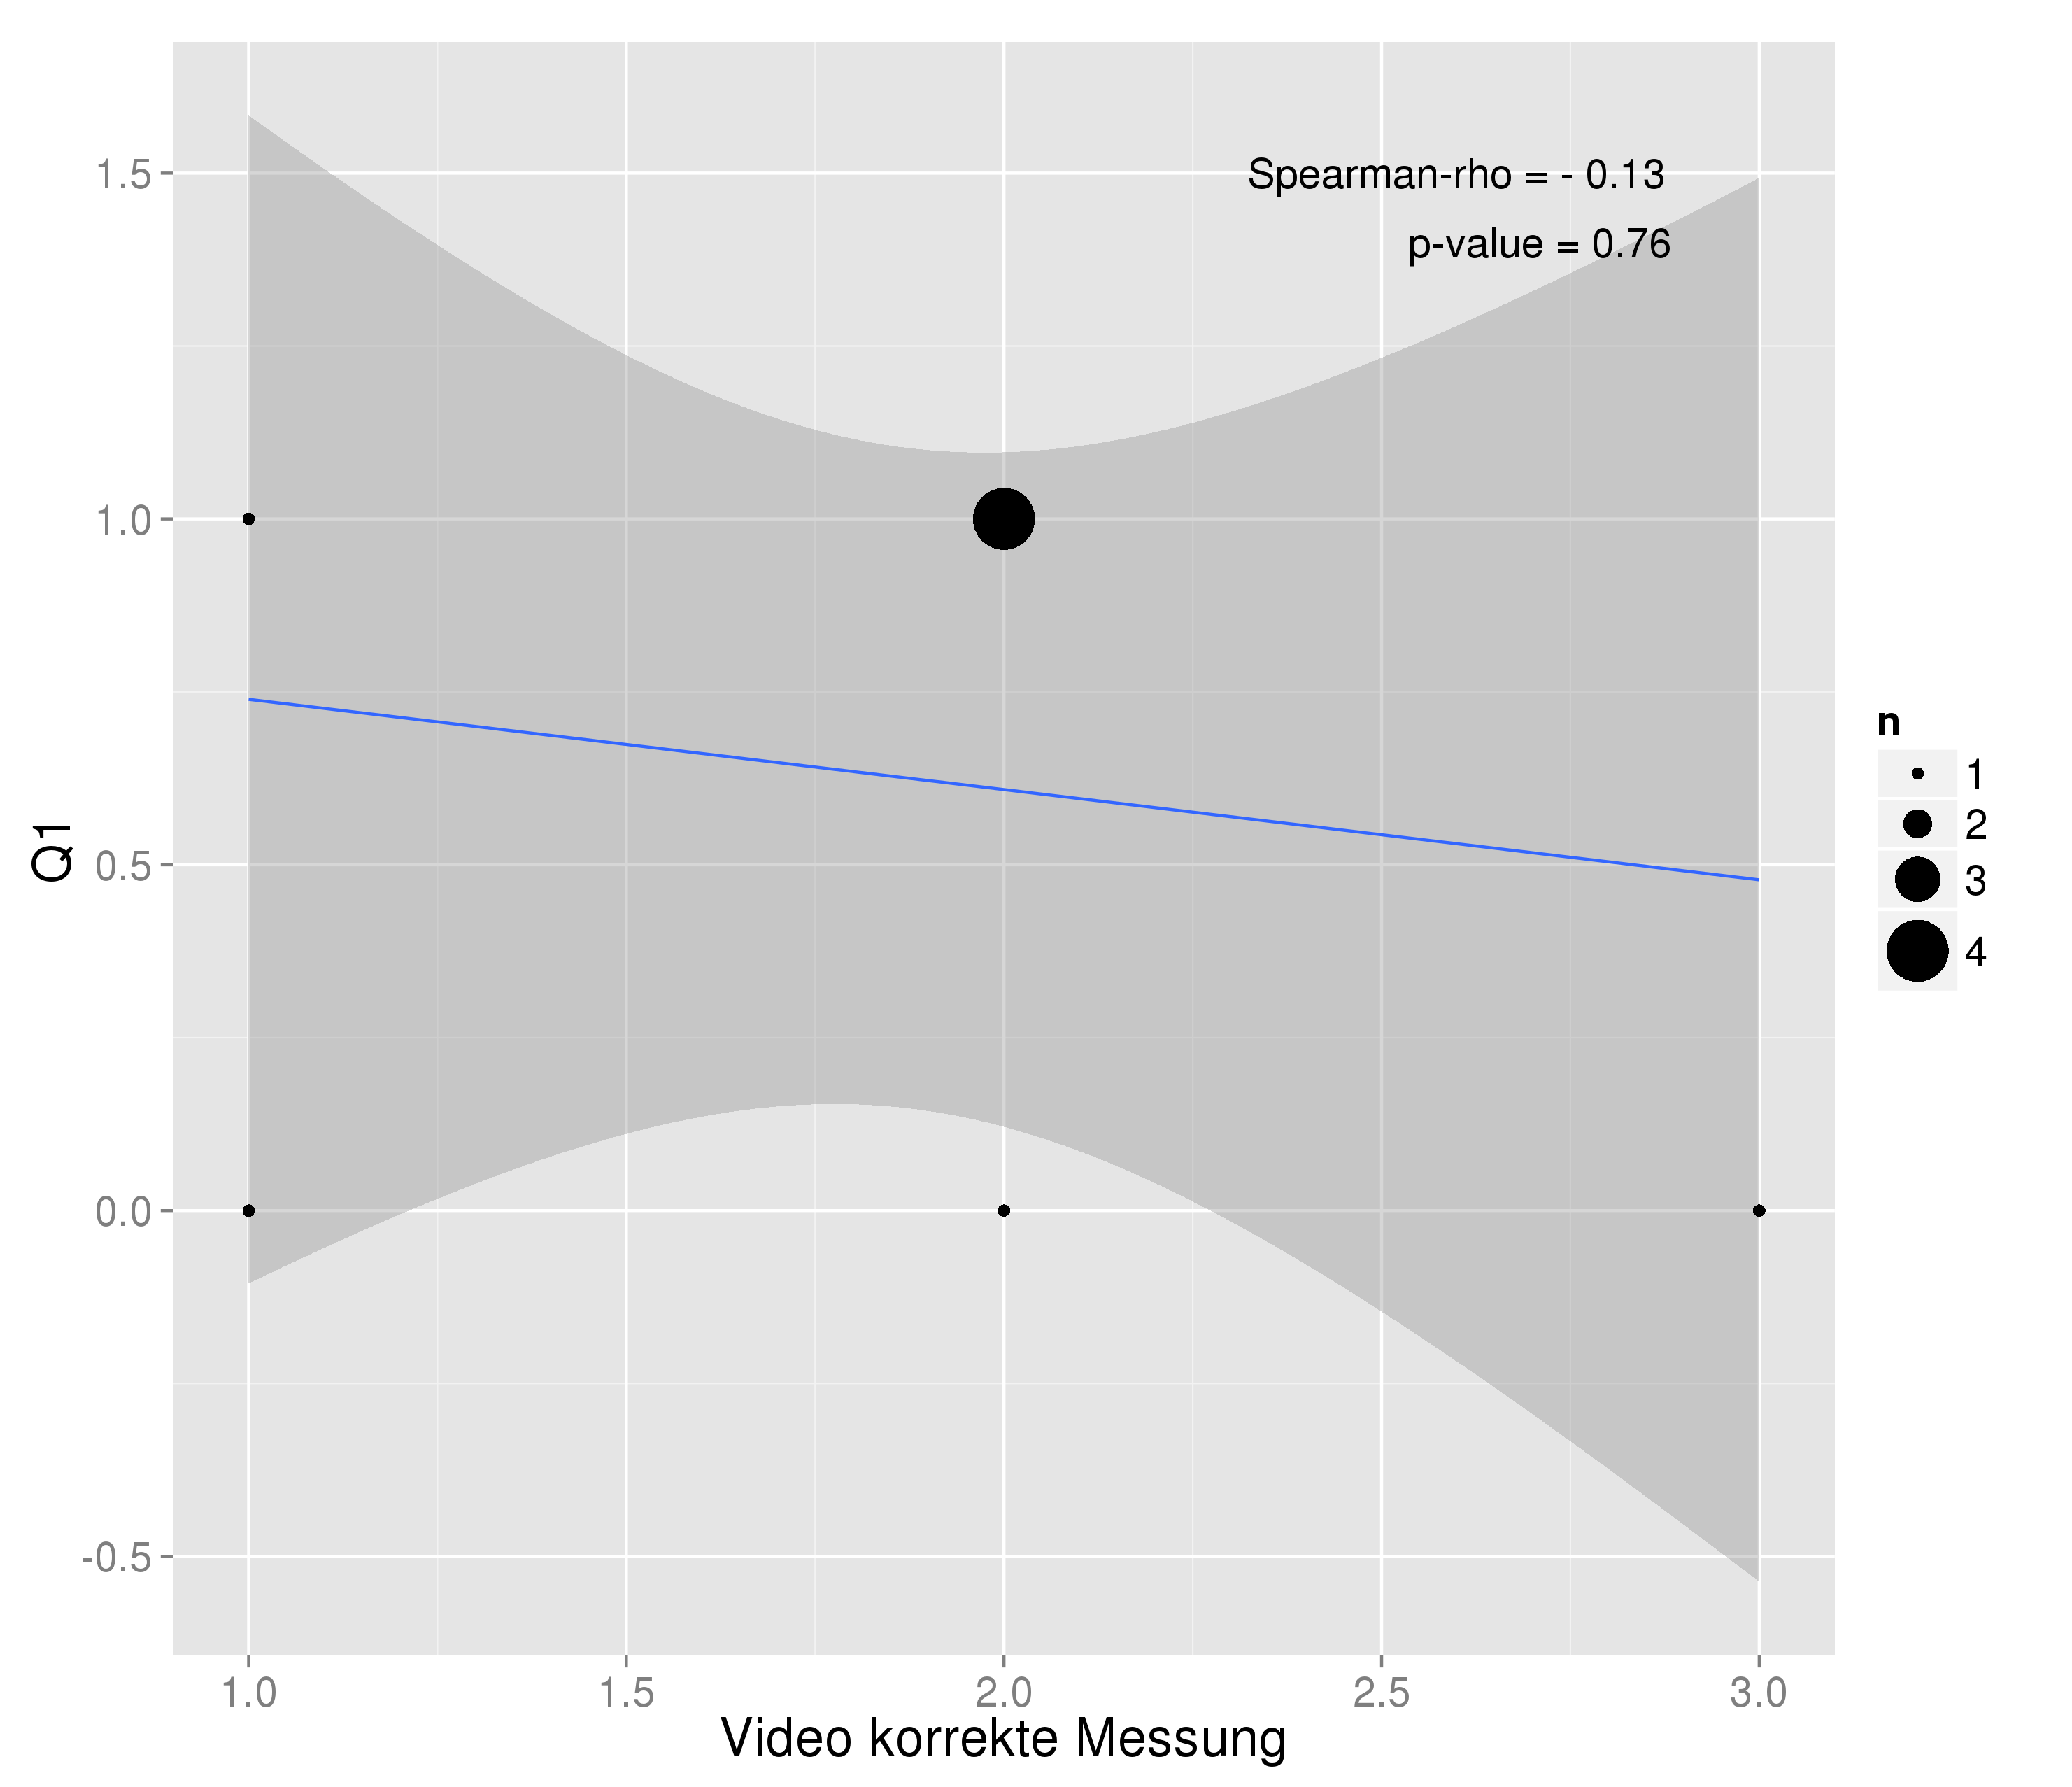
\includegraphics[width=1.0\linewidth]{graphics/corVideoQ1201.png}
    \caption{Vergleich Q1 mit Merkmal korrekte Messung für Test 201.}
    \label{fig:corVideoQ1201}
  \end{subfigure}
  \begin{subfigure}{0.32\textwidth}
    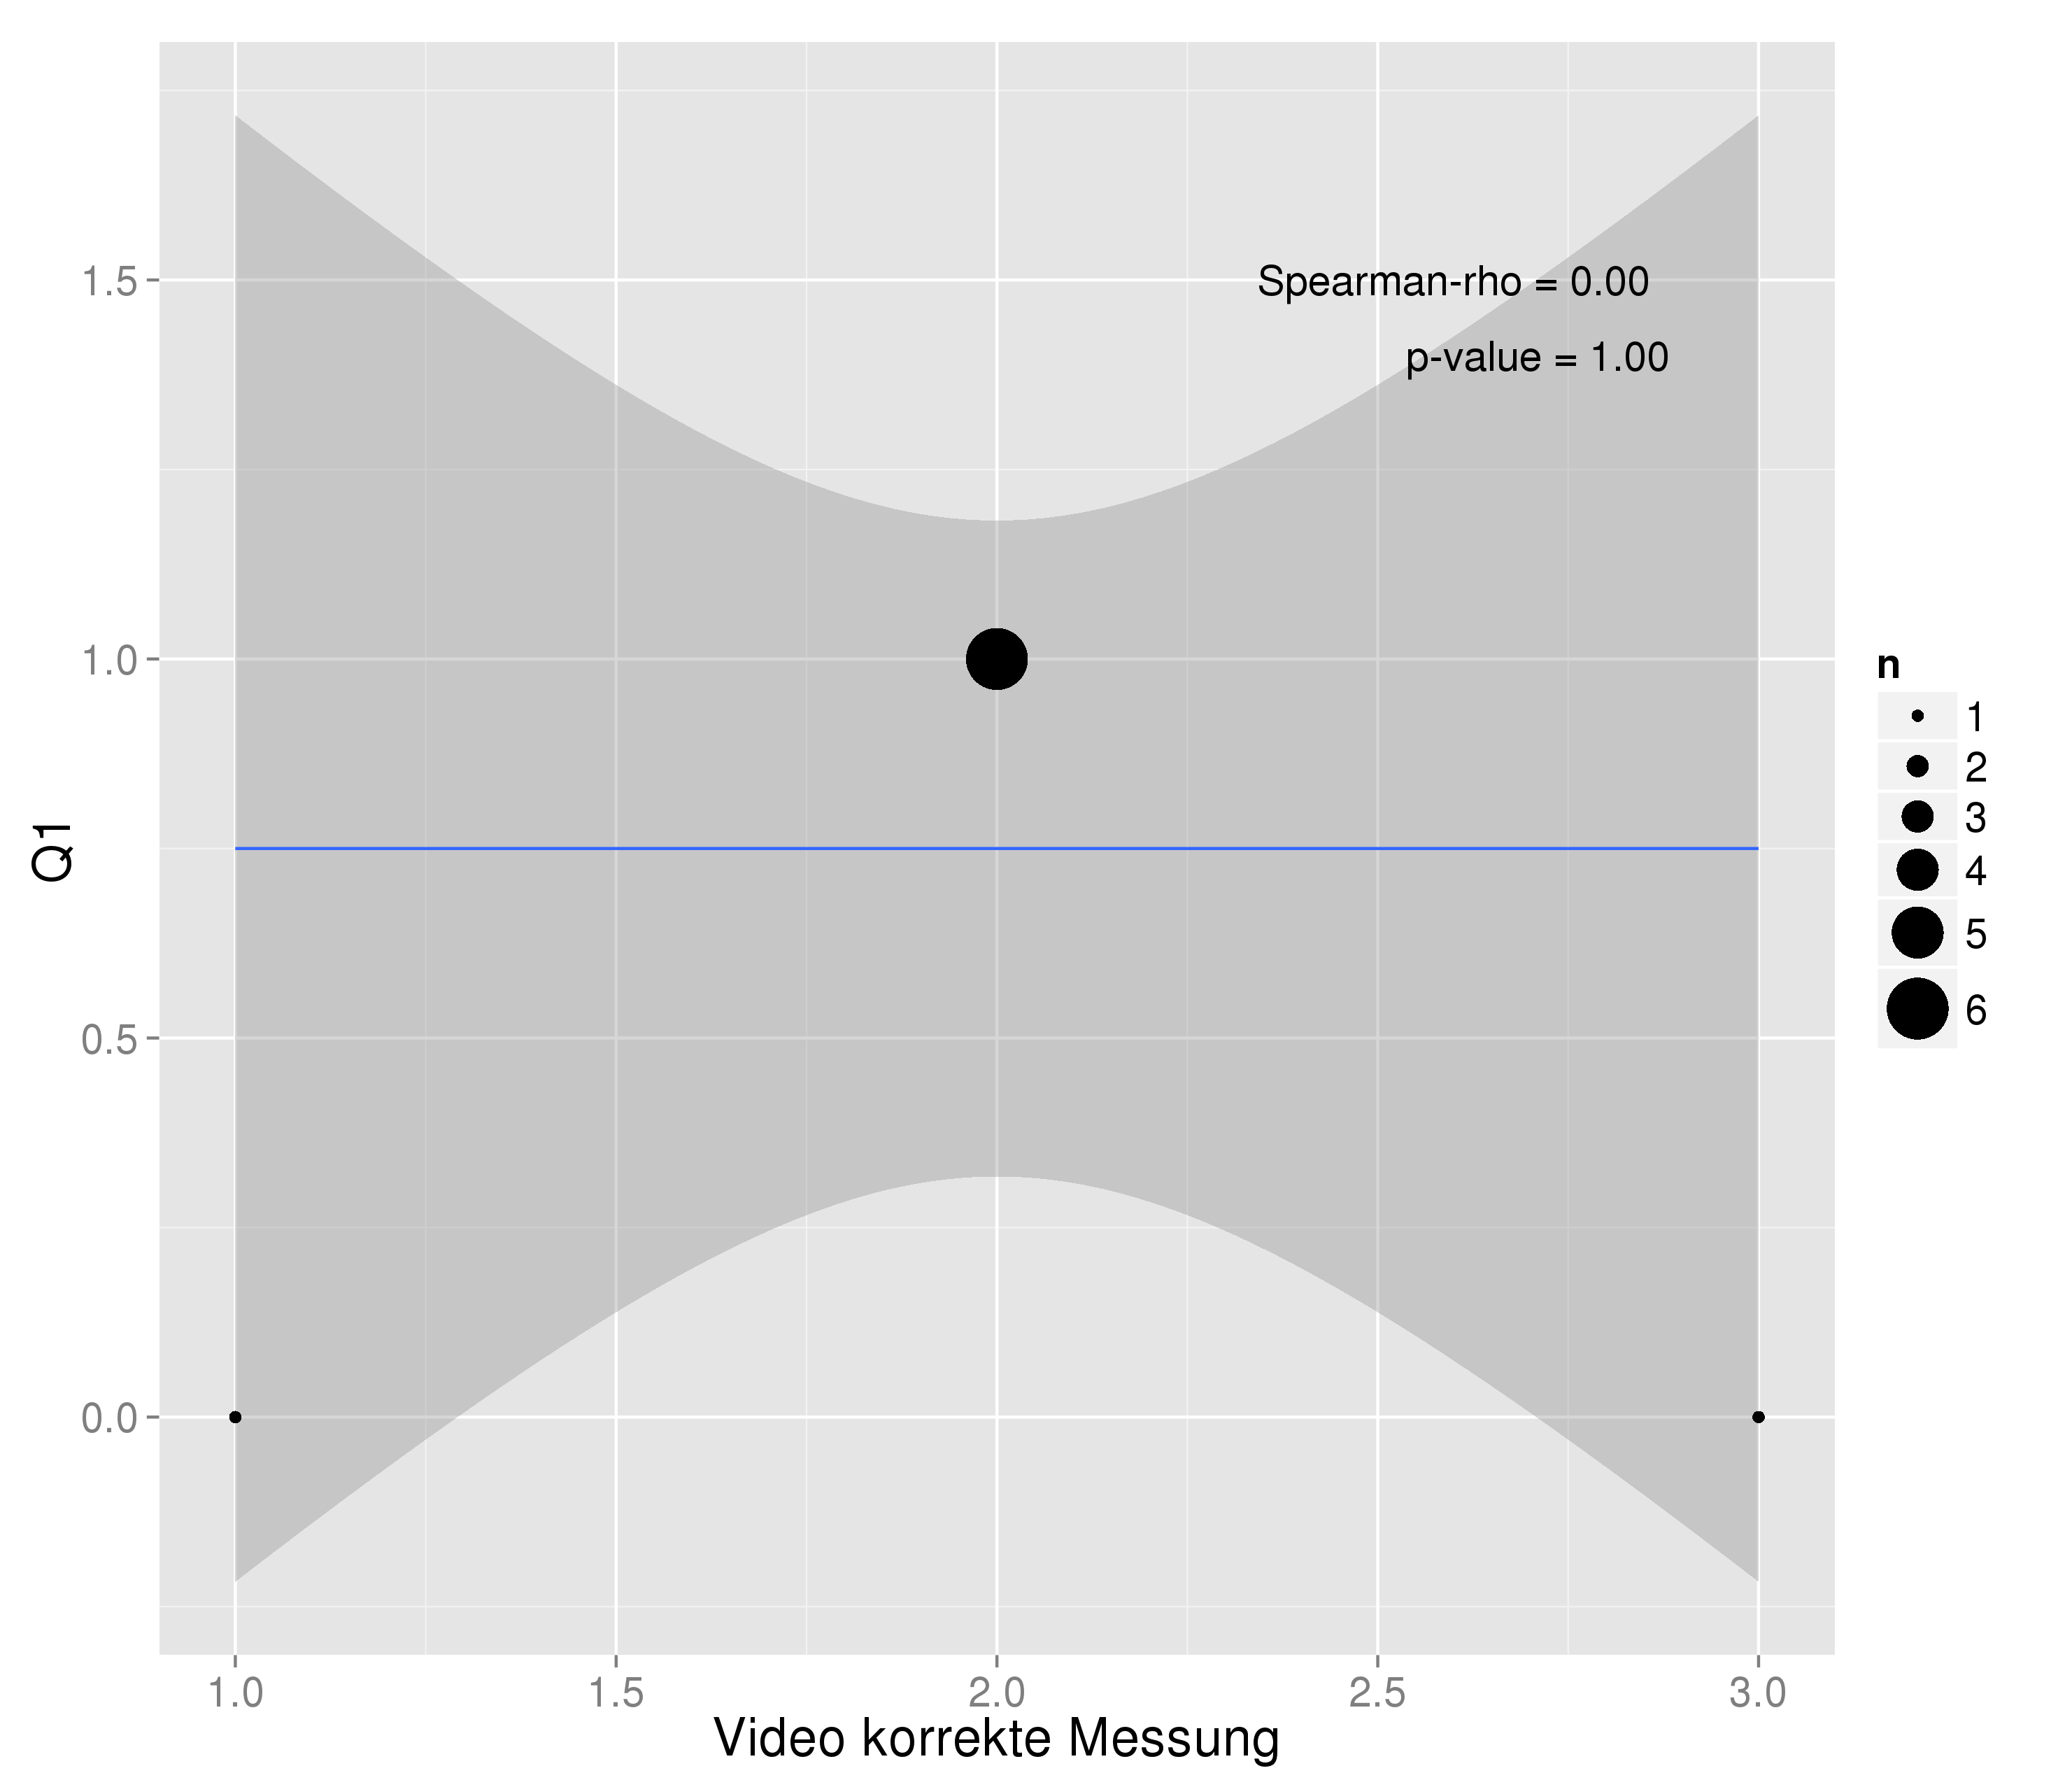
\includegraphics[width=1.0\linewidth]{graphics/corVideoQ1301.png}
    \caption{Vergleich Q1 mit Merkmal korrekte Messung für Test 301.}
    \label{fig:corVideoQ1301}
  \end{subfigure}
  \begin{subfigure}{0.32\textwidth}
      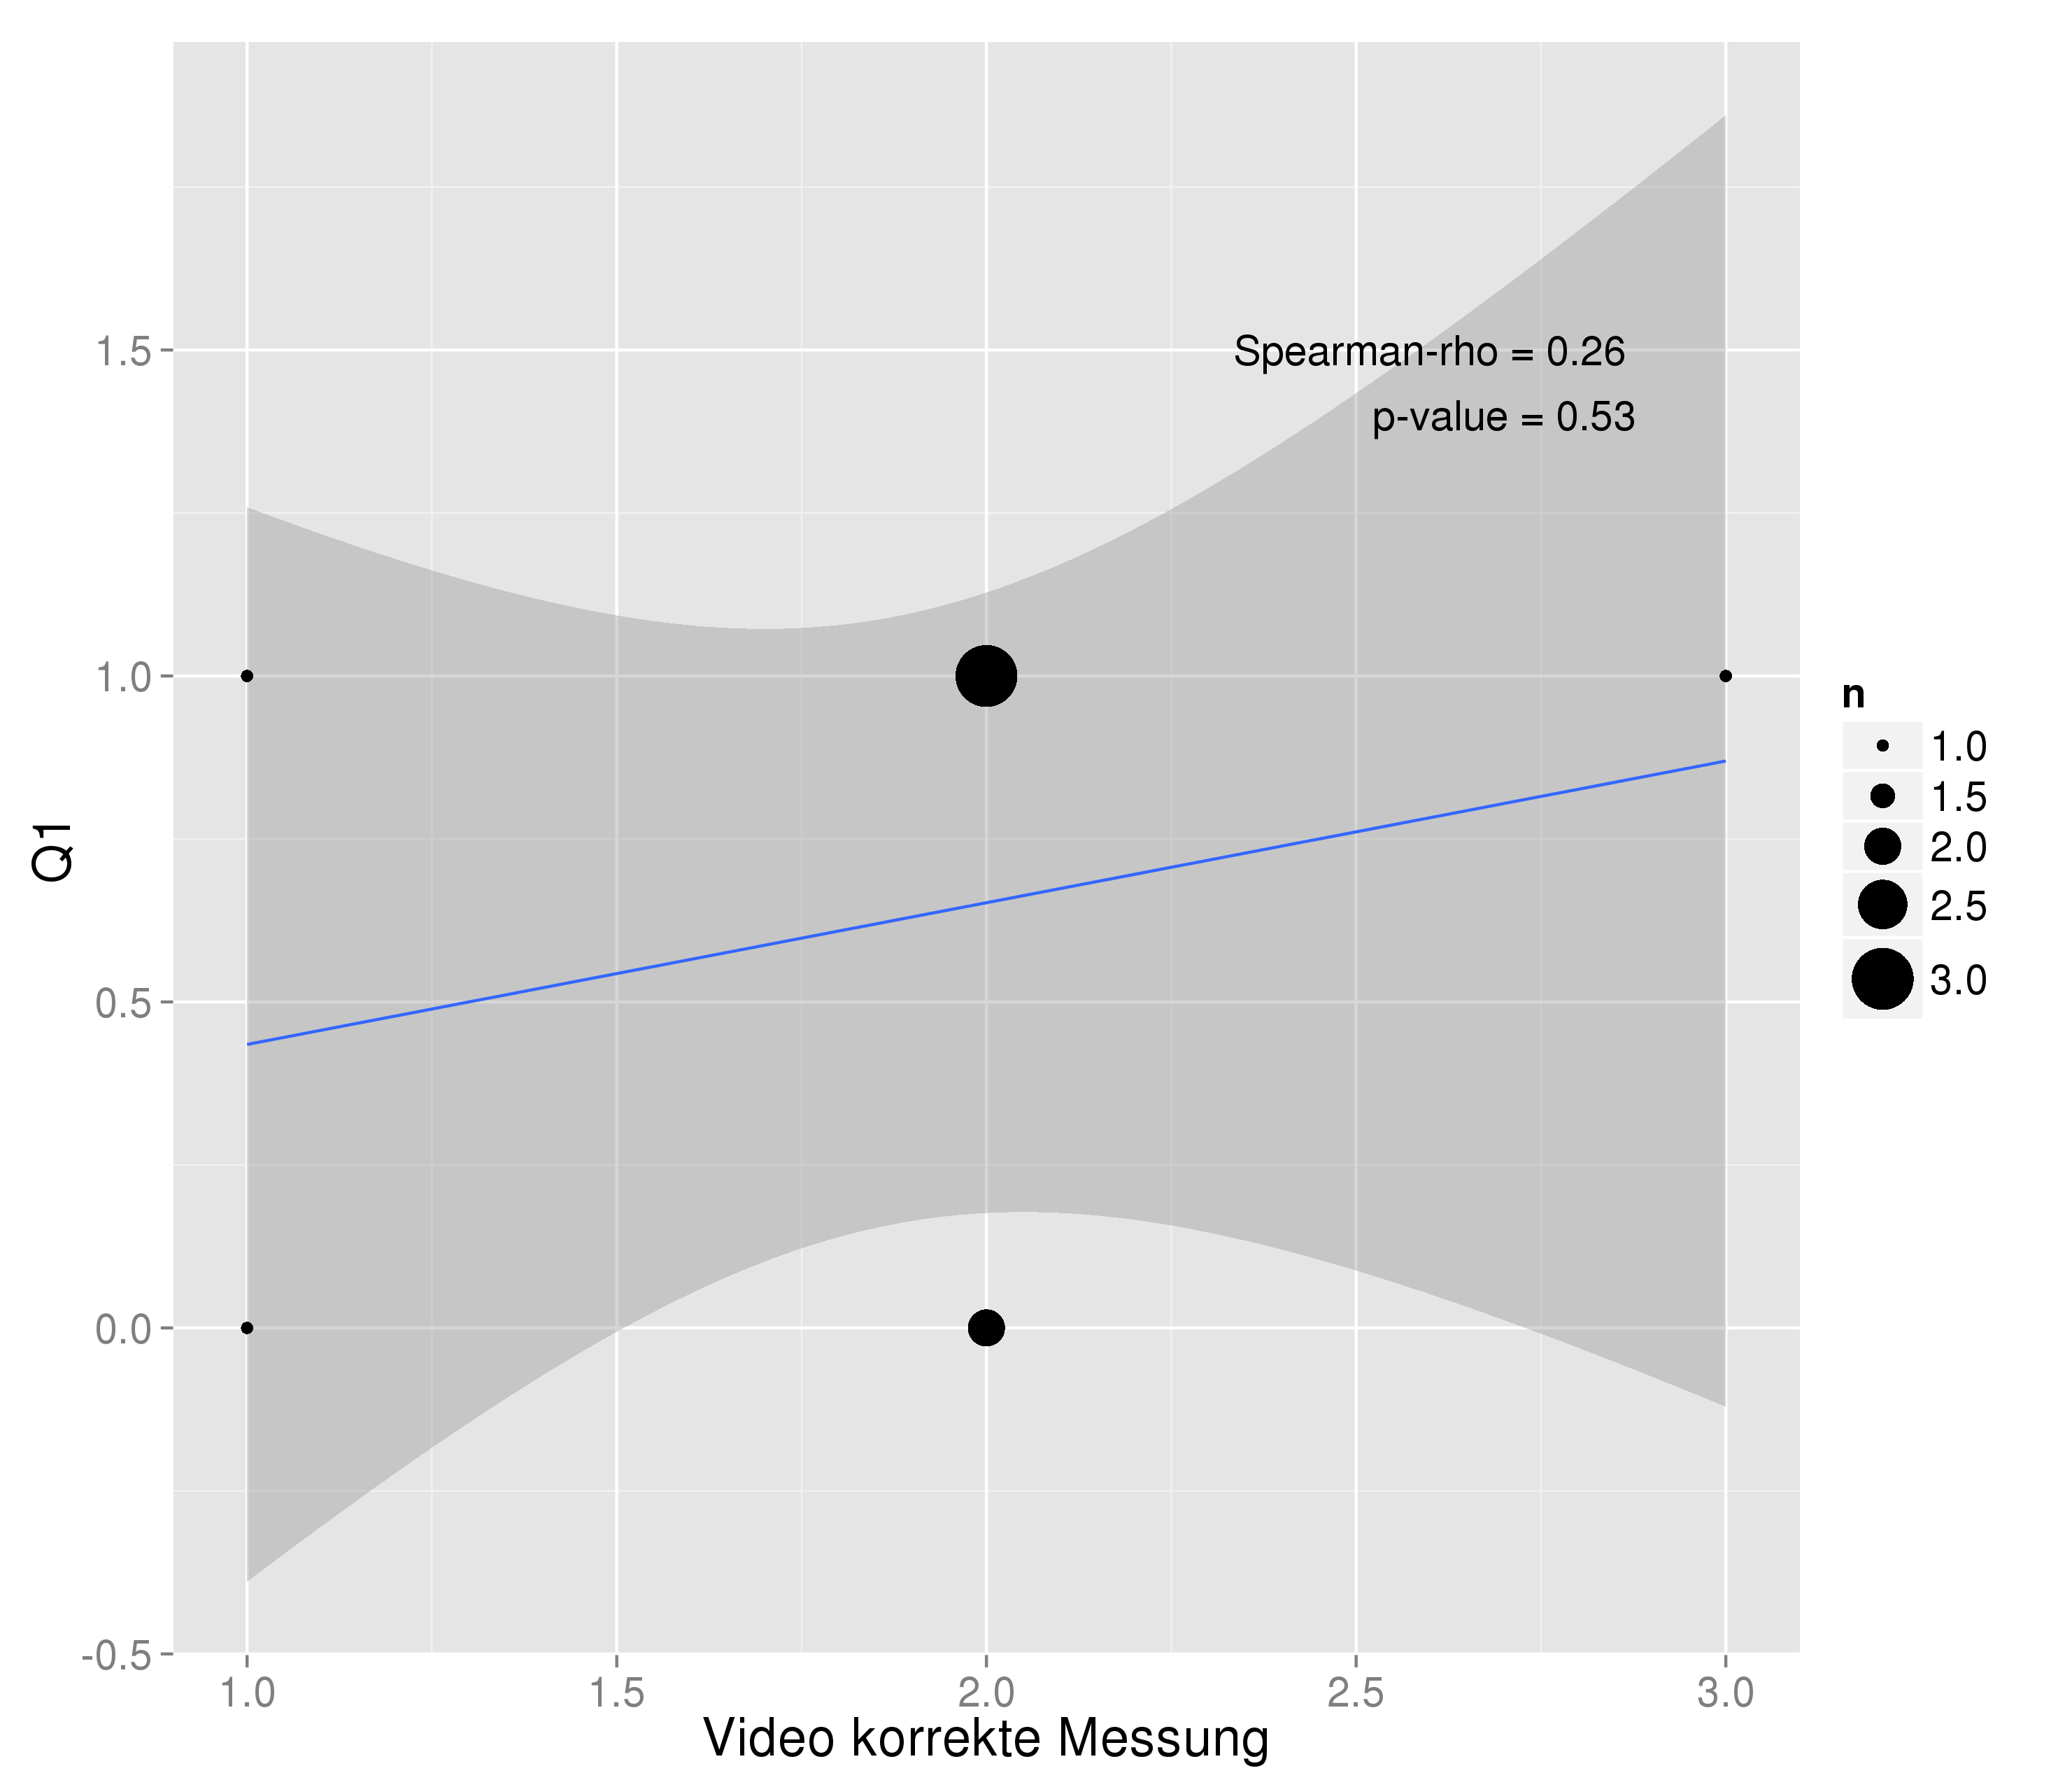
\includegraphics[width=1.0\linewidth]{graphics/corVideoQ1305.png}
    \caption{Vergleich Q1 mit Merkmal korrekte Messung für Test 305.}
    \label{fig:corVideoQ1305}
   \end{subfigure}
 
   \begin{subfigure}{0.32\textwidth}
       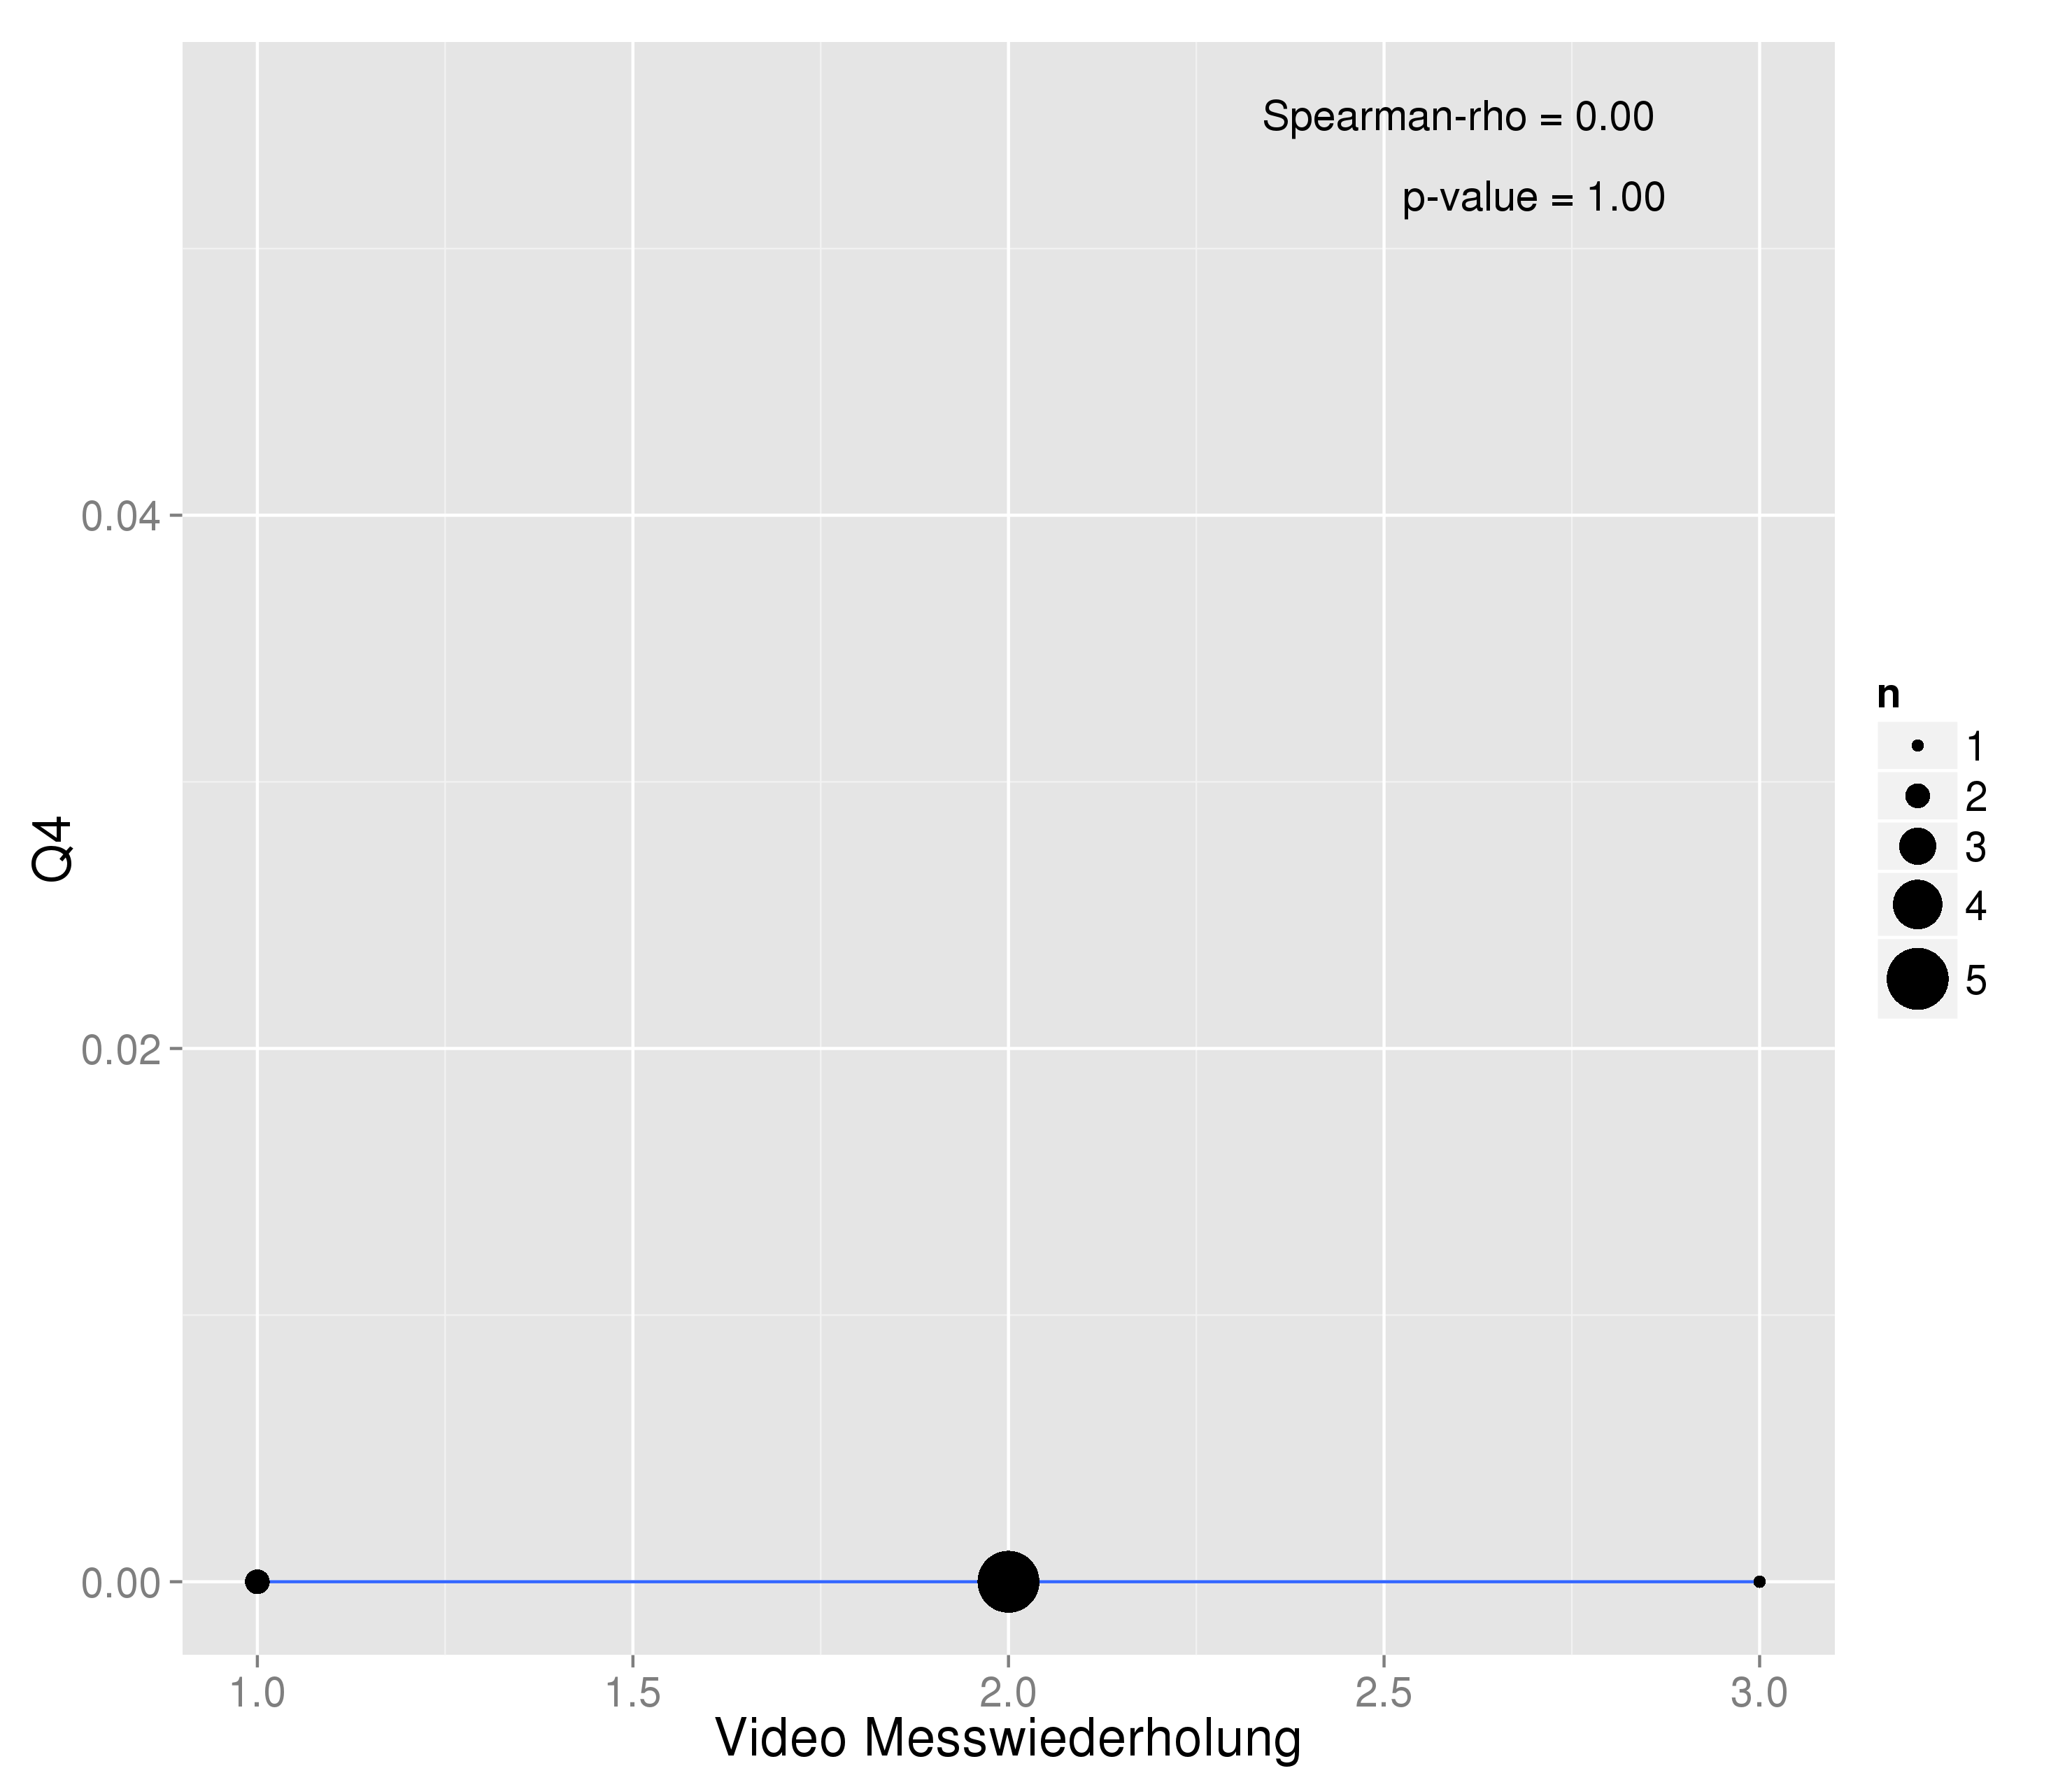
\includegraphics[width=1.0\linewidth]{graphics/corVideoQ4201.png}
       \caption{Vergleich Q4 mit Merkmal korrekte Messung für Test 201.}
       \label{fig:corVideoQ4201}
     \end{subfigure}
     \begin{subfigure}{0.32\textwidth}
       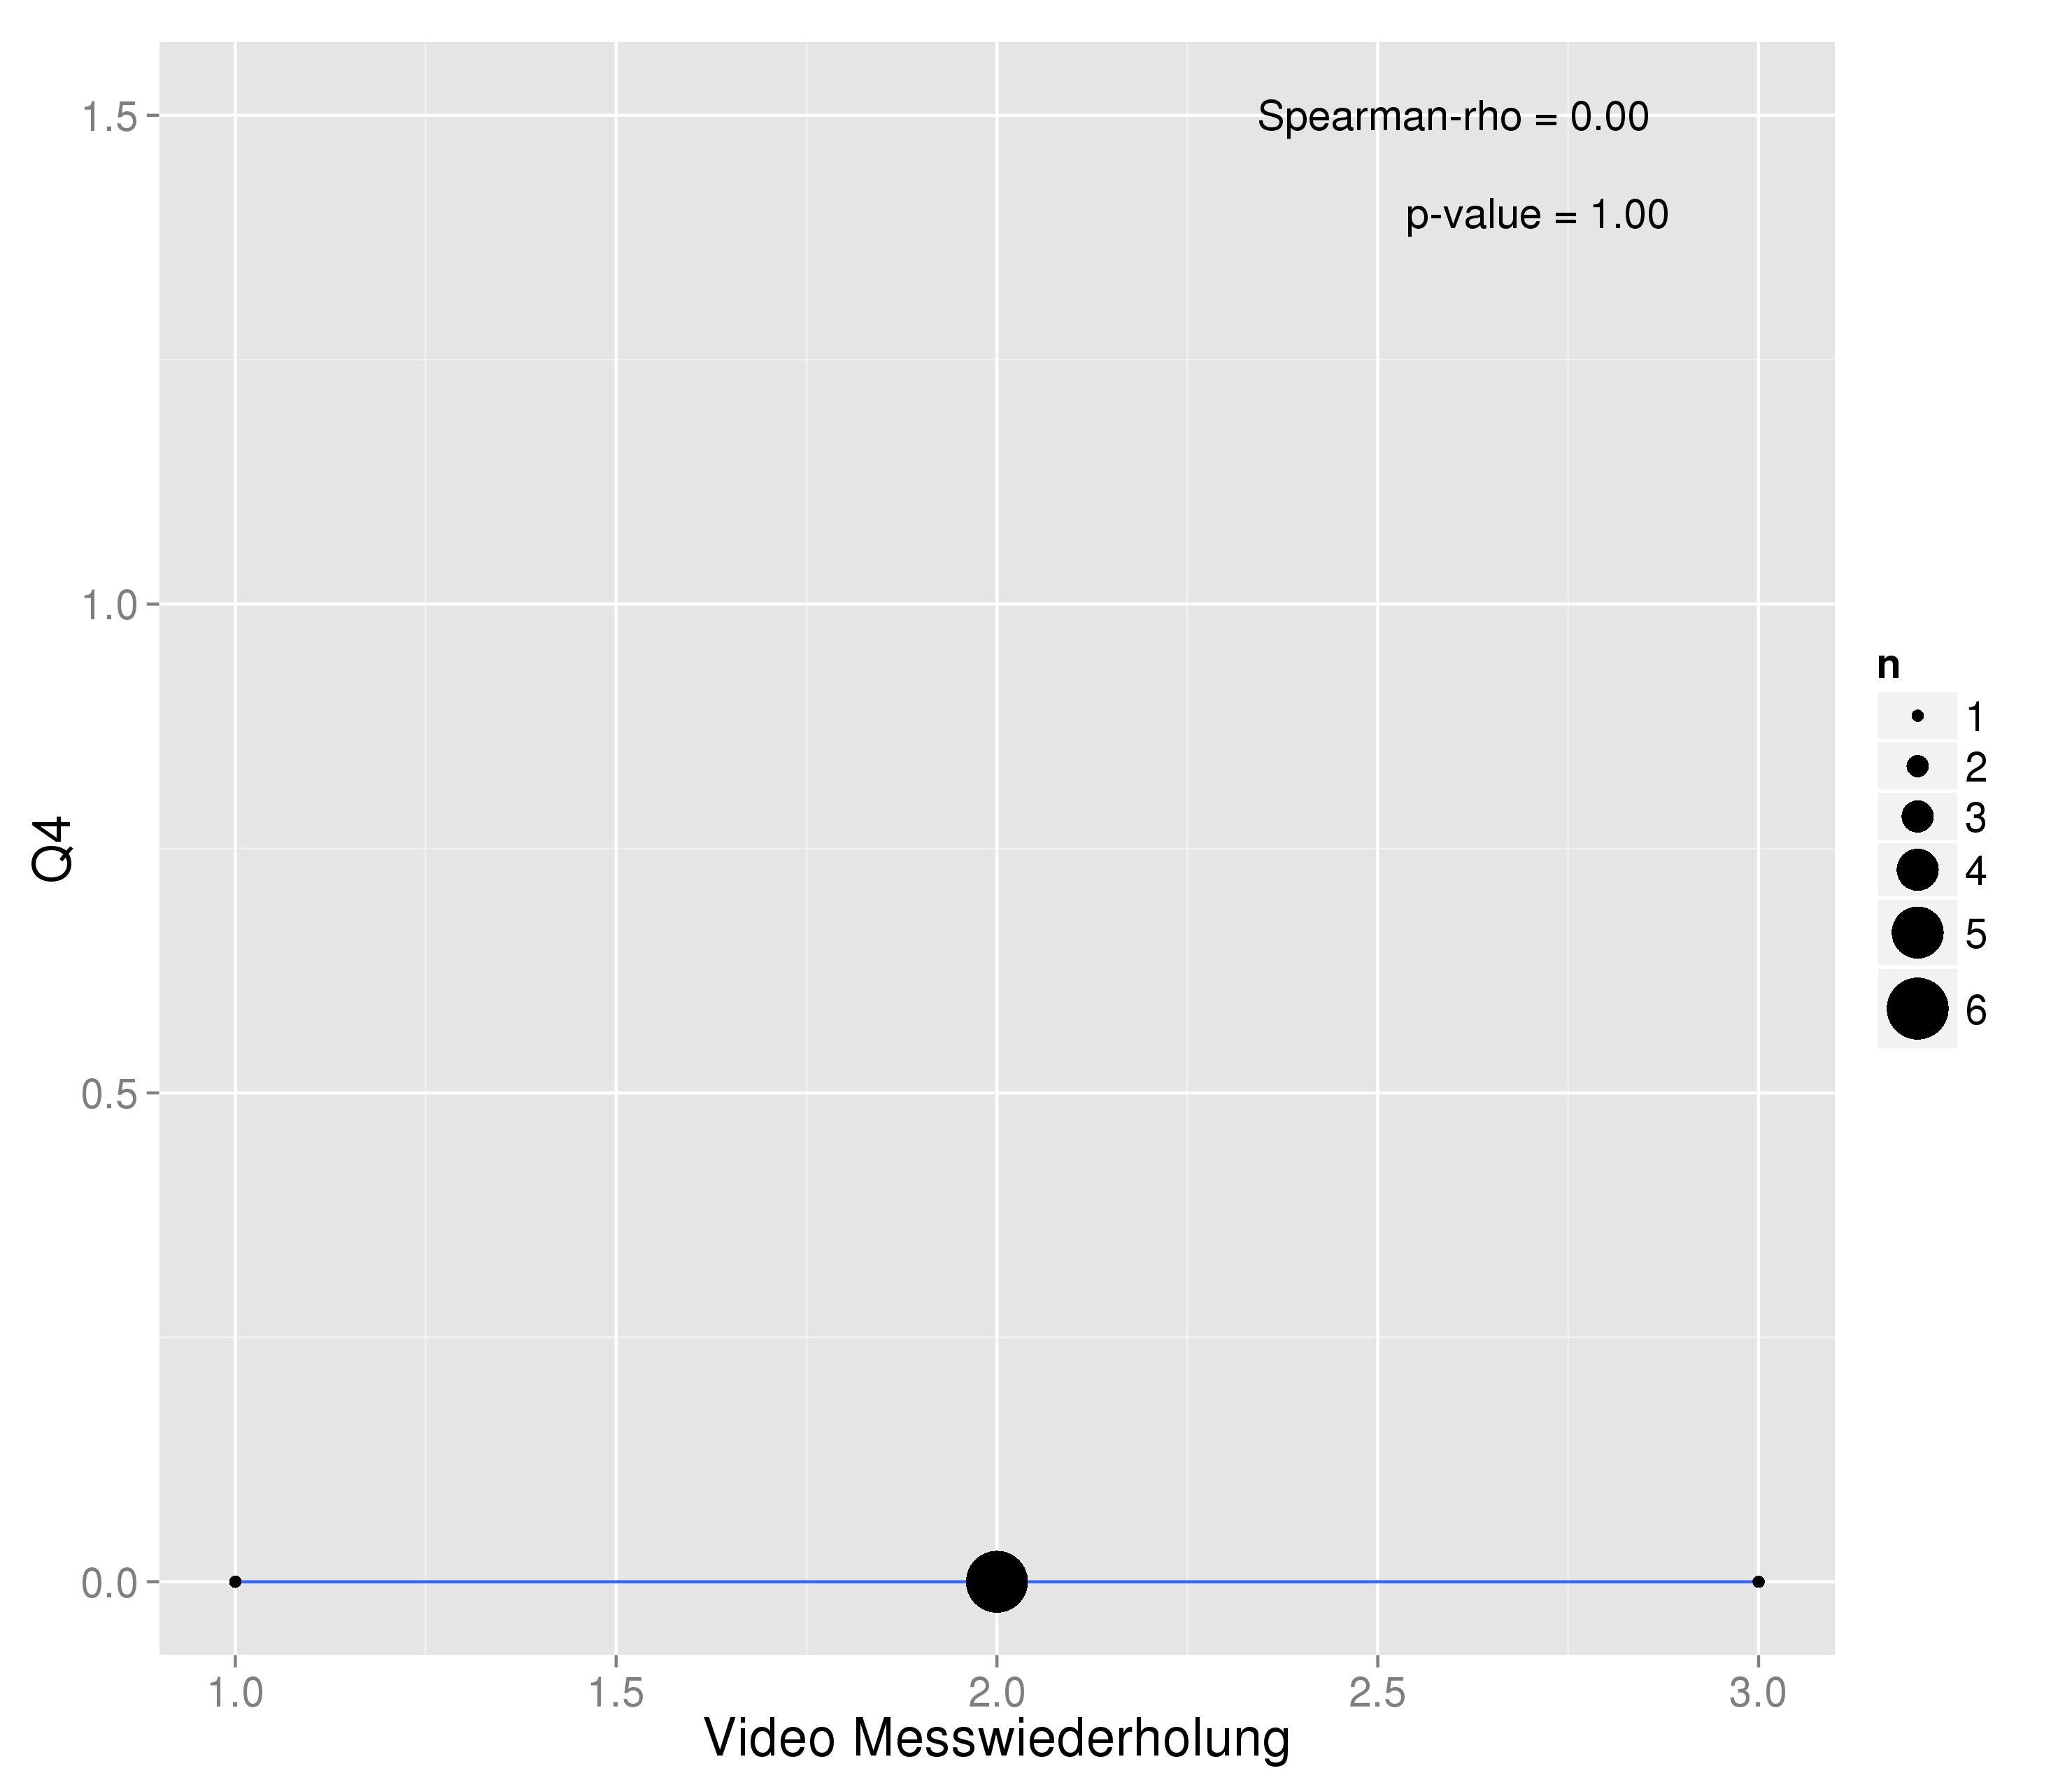
\includegraphics[width=1.0\linewidth]{graphics/corVideoQ4301.png}
       \caption{Vergleich Q4 mit Merkmal korrekte Messung für Test 301.}
       \label{fig:corVideoQ4301}
     \end{subfigure}
      \begin{subfigure}{0.32\textwidth}
         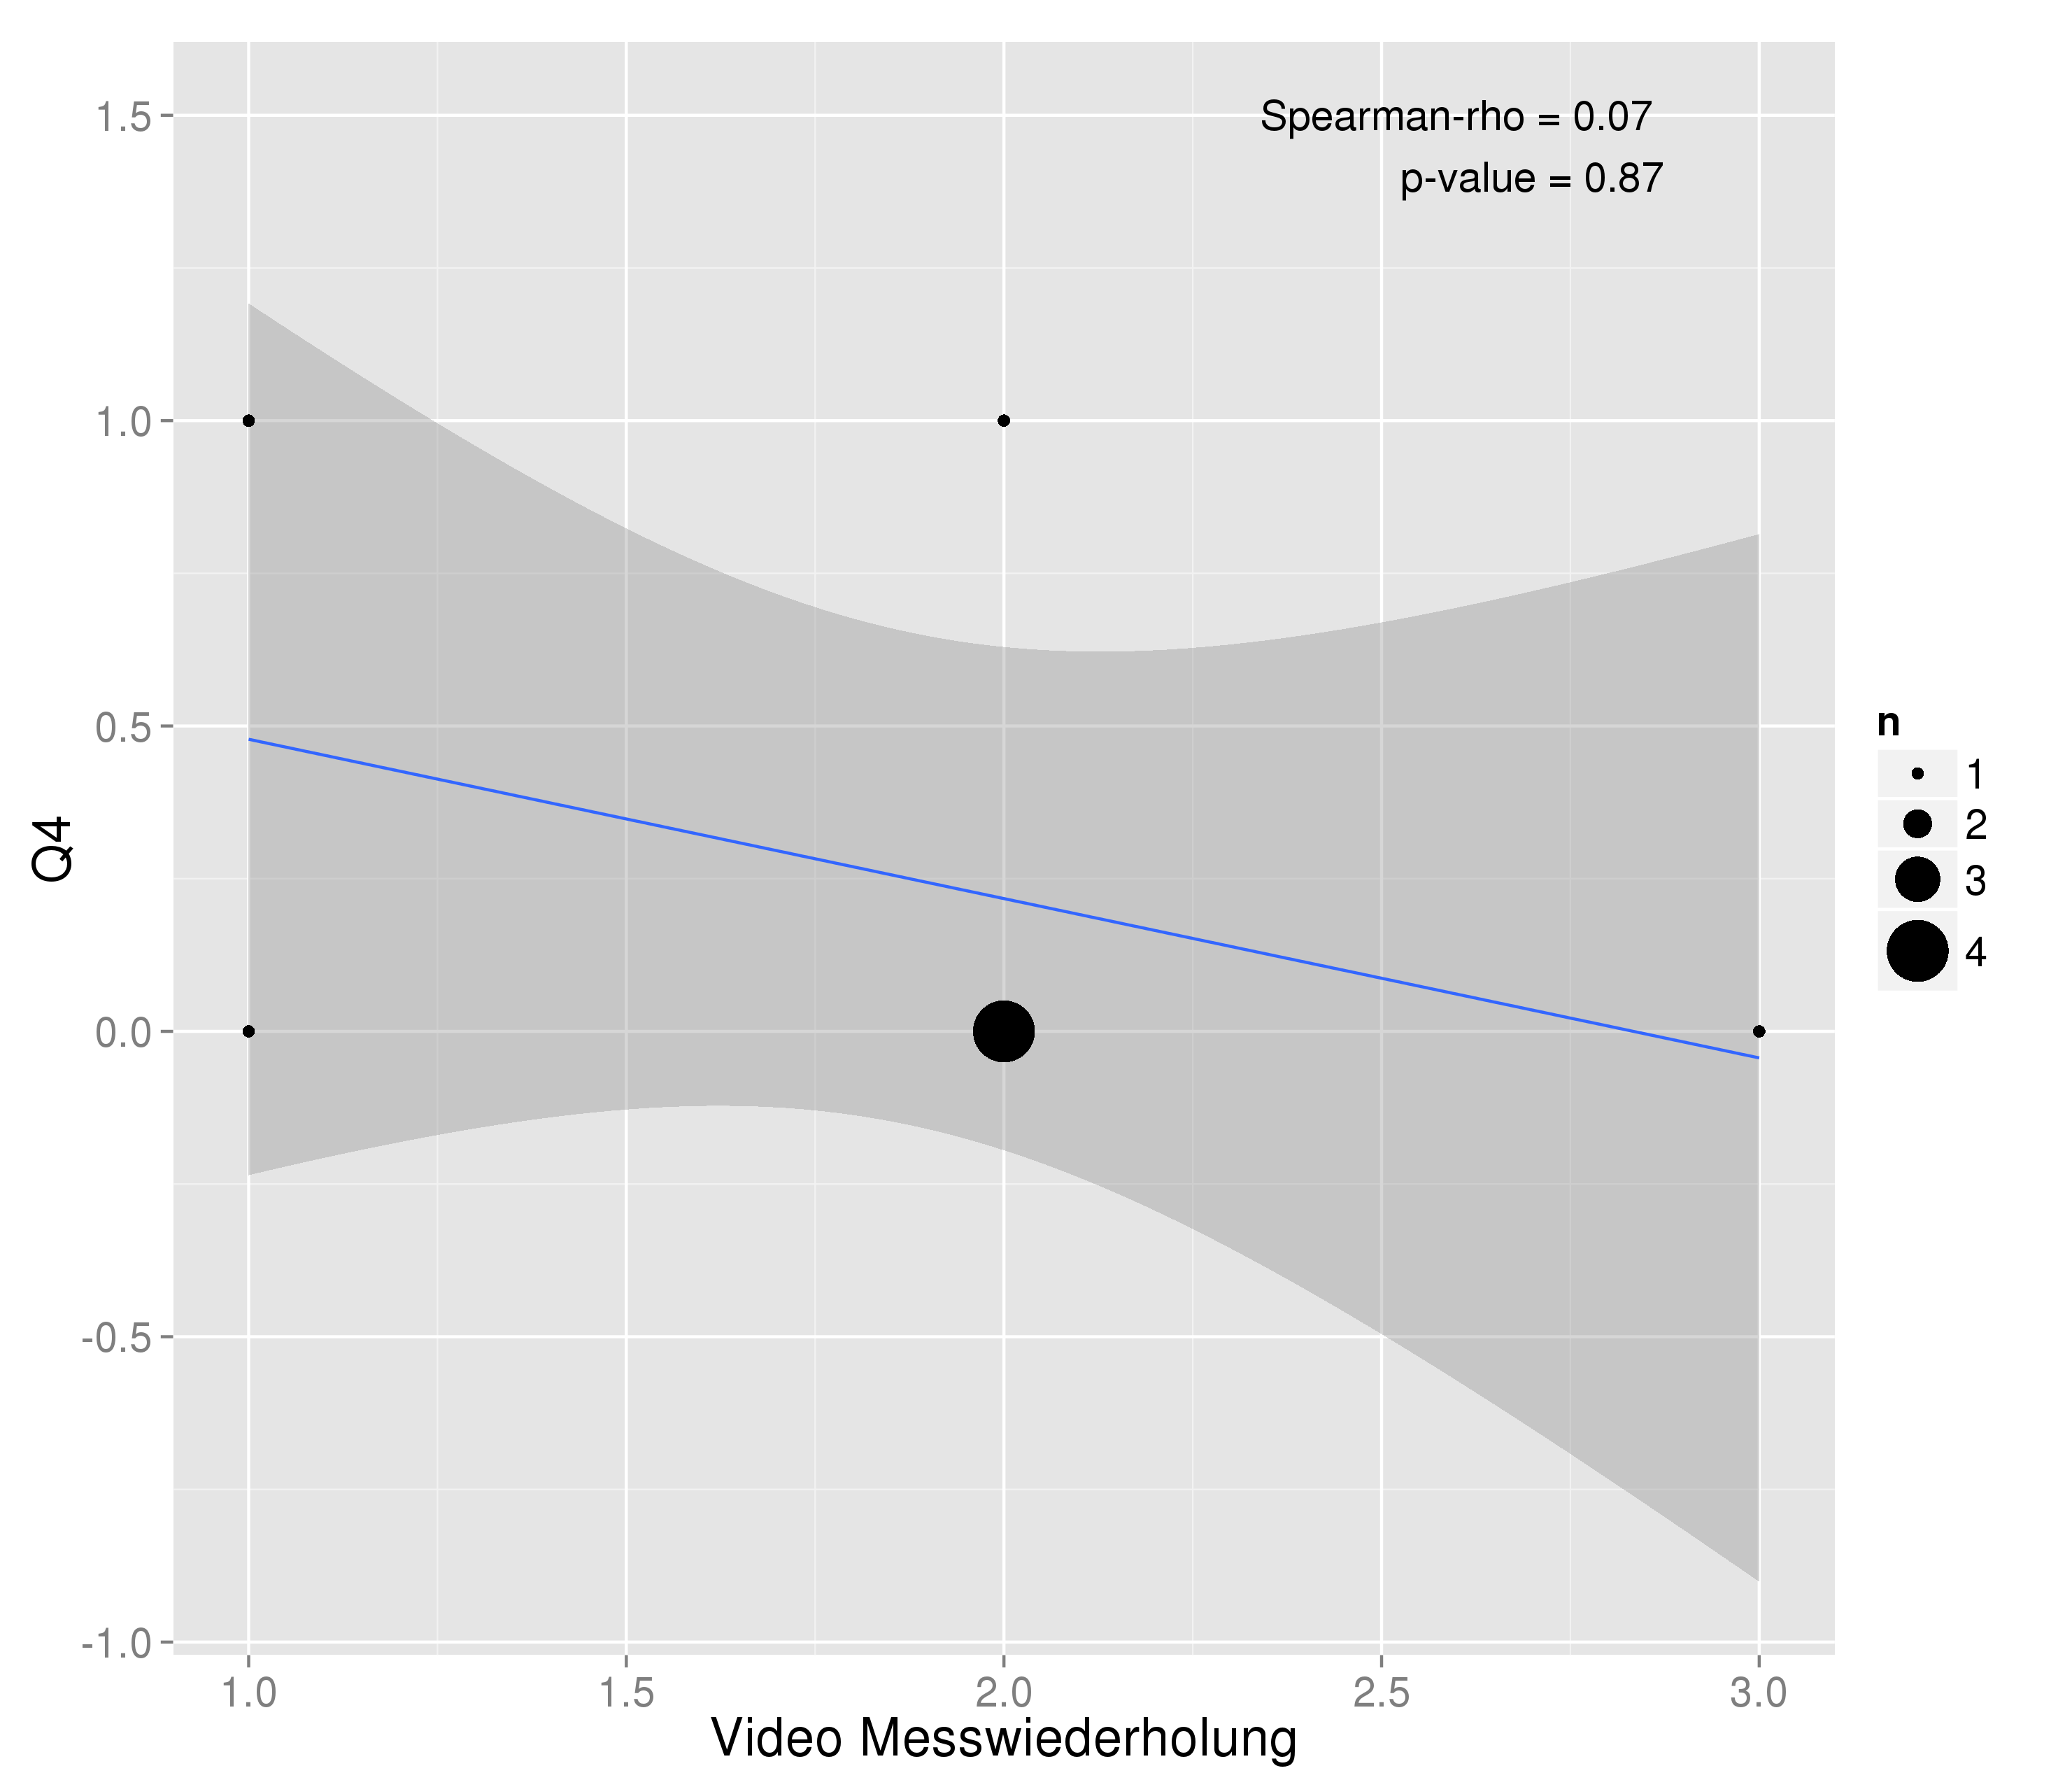
\includegraphics[width=1.0\linewidth]{graphics/corVideoQ4305.png}
       \caption{Vergleich Q4 mit Merkmal korrekte Messung für Test 305.}
       \label{fig:corVideoQ4305}
       \end{subfigure}
  
  \caption{Vergleich der Merkmale der Videokodierung mit den Qualitätsstandards 1 und 4. Der Durchmesser der Punkte ist ein Mass für die Anzahl an Datenpunkten, welche an dieser Position liegen. Die blaue Gerade ist die lineare Regression der zugrunde liegenden Daten, der dunkel graue Bereich stellt das Vertrauensintervall (95\%) der linearen Regression dar. Zusätzlich sind noch Spearmans $rho$ und der p-Wert des Signifikanztests angegeben.}
  \label{fig:corVideoQ}
  \end{figure}
 
 \begin{table}[htbp]
   \centering
 \begin{tabular}{@{}lllllllllll@{}}
 \toprule
    \multicolumn{2}{l}{201 Q1} &&  \multicolumn{2}{l}{201 Q4}&&  \multicolumn{2}{l}{301 Q1}&&  \multicolumn{2}{l}{301 Q4} \\ 
       \cmidrule{1-2}\cmidrule{4-5}\cmidrule{7-8}\cmidrule{10-11}
    p-Wert & $\rho$ && p-Wert & $\rho$  && p-Wert & $\rho$&& p-Wert & $\rho$\\ 
 \midrule
    0.76 & -0.13 && 1.00 & 0.0 && 1.00 & 0.0 && 1.00 & 0.0     \\ 
 
 \bottomrule
 \end{tabular} \\[0.75cm]
 \begin{tabular}{@{}lllll@{}}
  \toprule
       \multicolumn{2}{l}{305 Q1}&&  \multicolumn{2}{l}{305 Q4}\\ 
        \cmidrule{1-2}\cmidrule{4-5}
      p-Wert & $\rho$&& p-Wert & $\rho$\\ 
  \midrule
      0.53 & 0.26 && 0.87 & 0.07    \\ 
  
  \bottomrule
  \end{tabular} 
   \caption{Spearmans $\rho$ und p-Werte für die Korrelation zwischen Qualitätsstandards und den Merkmalen aus der Videokodierung..  }
   \label{tab:CorVideoQ}
 \end{table}
 
  \subsection{Messzeitpunkte und Messdauer}
  
  Zusätzlich zu den zwei Merkmalen wurde für jede Messung noch erhoben, wann die Messung begonnen hatte und wann die Messung beendet wurde. Bei der Temperaturmessung war die Definition der Messung nicht trivial. Es wurde folgende Definition für eine Messung verwendet. Für eine Temperaturmessung, muss dass Thermometer aus dem Medium entfernt werden und abgelesen werden. Ein Ablesen ohne, dass das Thermometer aus dem Medium herausgenommen wird, gilt nicht als Messung. Der Hauptgrund für diese eingeschränkte Definition ist, dass der Ablese-Vorgang nur sehr schwierig eindeutig beobachtbar ist. Daher wurde dieser mit dem Entfernen des Thermometers verknüpft, sodass die Kodierung einfacher ist. Ein Problem dabei war der Test 201, da dort die Thermometer über das Video nicht unterscheidbar waren. Daher wurden dort die Messinstrumente mit 1 und 2 kodiert. Die Resultate finden sich in Darstellung \ref{fig:Messungen}.
  
  
  
   \begin{figure}[htp]
   \centering
   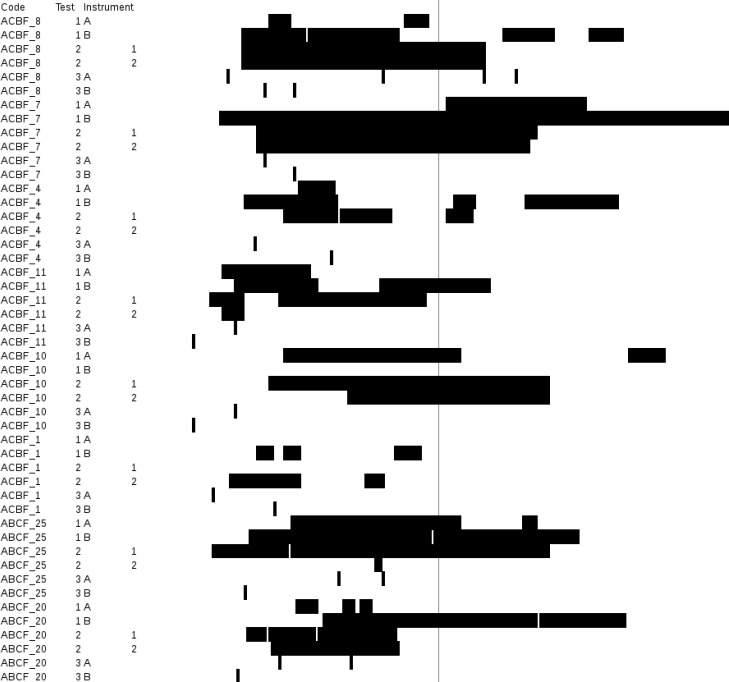
\includegraphics[width=1.0\linewidth]{graphics/Messungen2.png}
   \caption{Übersicht über alle Messungen der Videografierten Schülerinnen und Schülern. In der ersten Spalte die der Identifizierungs-Code. In der Spalte 2 welcher Test wobei gilt 1 = 305, 2 = 201, 3 = 301. In Schwarz wird jeweils markiert wenn eine Messung durchgeführt wird. Die Linie in der Mitte entspricht der Halbzeit des Testes (10 min)}
   \label{fig:Messungen}
   \end{figure}
   
   \github{http://git.io/bvQS}
  